\documentclass[14pt,xcolor=dvipsnames,table,dvipdfmx]{beamer}

\usepackage{slide}
\usepackage{appendixnumberbeamer}

\usepackage{math_macros}

\usepackage{import}
\usepackage{url}
\usepackage{diagbox}
\usepackage{array,colortbl}
\usepackage{hyperref}
% \hypersetup{
%     colorlinks=true,
%     citebordercolor=blue,
%     linkbordercolor=blue,
%     urlbordercolor=blue,
%     %citecolor=black,
% }
\usepackage{nicematrix}

\usepackage{booktabs}
\usepackage{caption}
\usepackage{dashrule}
\usepackage[normalem]{ulem}

\newcommand{\comment}[2]{\textcolor{green!35!black}{#1 \fbox{\scalebox{0.4}{#2}}}}

% 引用
% \usepackage[backend=bibtex, sorting=none]{biblatex}
\usepackage[sorting=none]{biblatex}
\addbibresource{./references.bib}
% 脚注に引用文献の情報を強引に乗せる
\newcommand*{\mycite}[1]{\parencite{#1} \citeauthor{#1} (\citeyear{#1})}
\renewcommand*{\footcite}[1]{\footnote{\mycite{#1}}}
\AtBeginBibliography{\scriptsize}

\title{MP3 (aka MPEG1-LayerIII)の\\要素技術}
\author[]{}
\date{2024.3-}

\begin{document}
\maketitle

\begin{frame}[c]
    \frametitle{あらすじ}
    % \tableofcontents[hideallsubsections]
    \tableofcontents
\end{frame}

\section{MP3概要}

\subsection{MPEG/Audioの歴史}

\begin{frame}[c]
    \frametitle{MPEG/Audioの歴史}
    \begin{figure}
        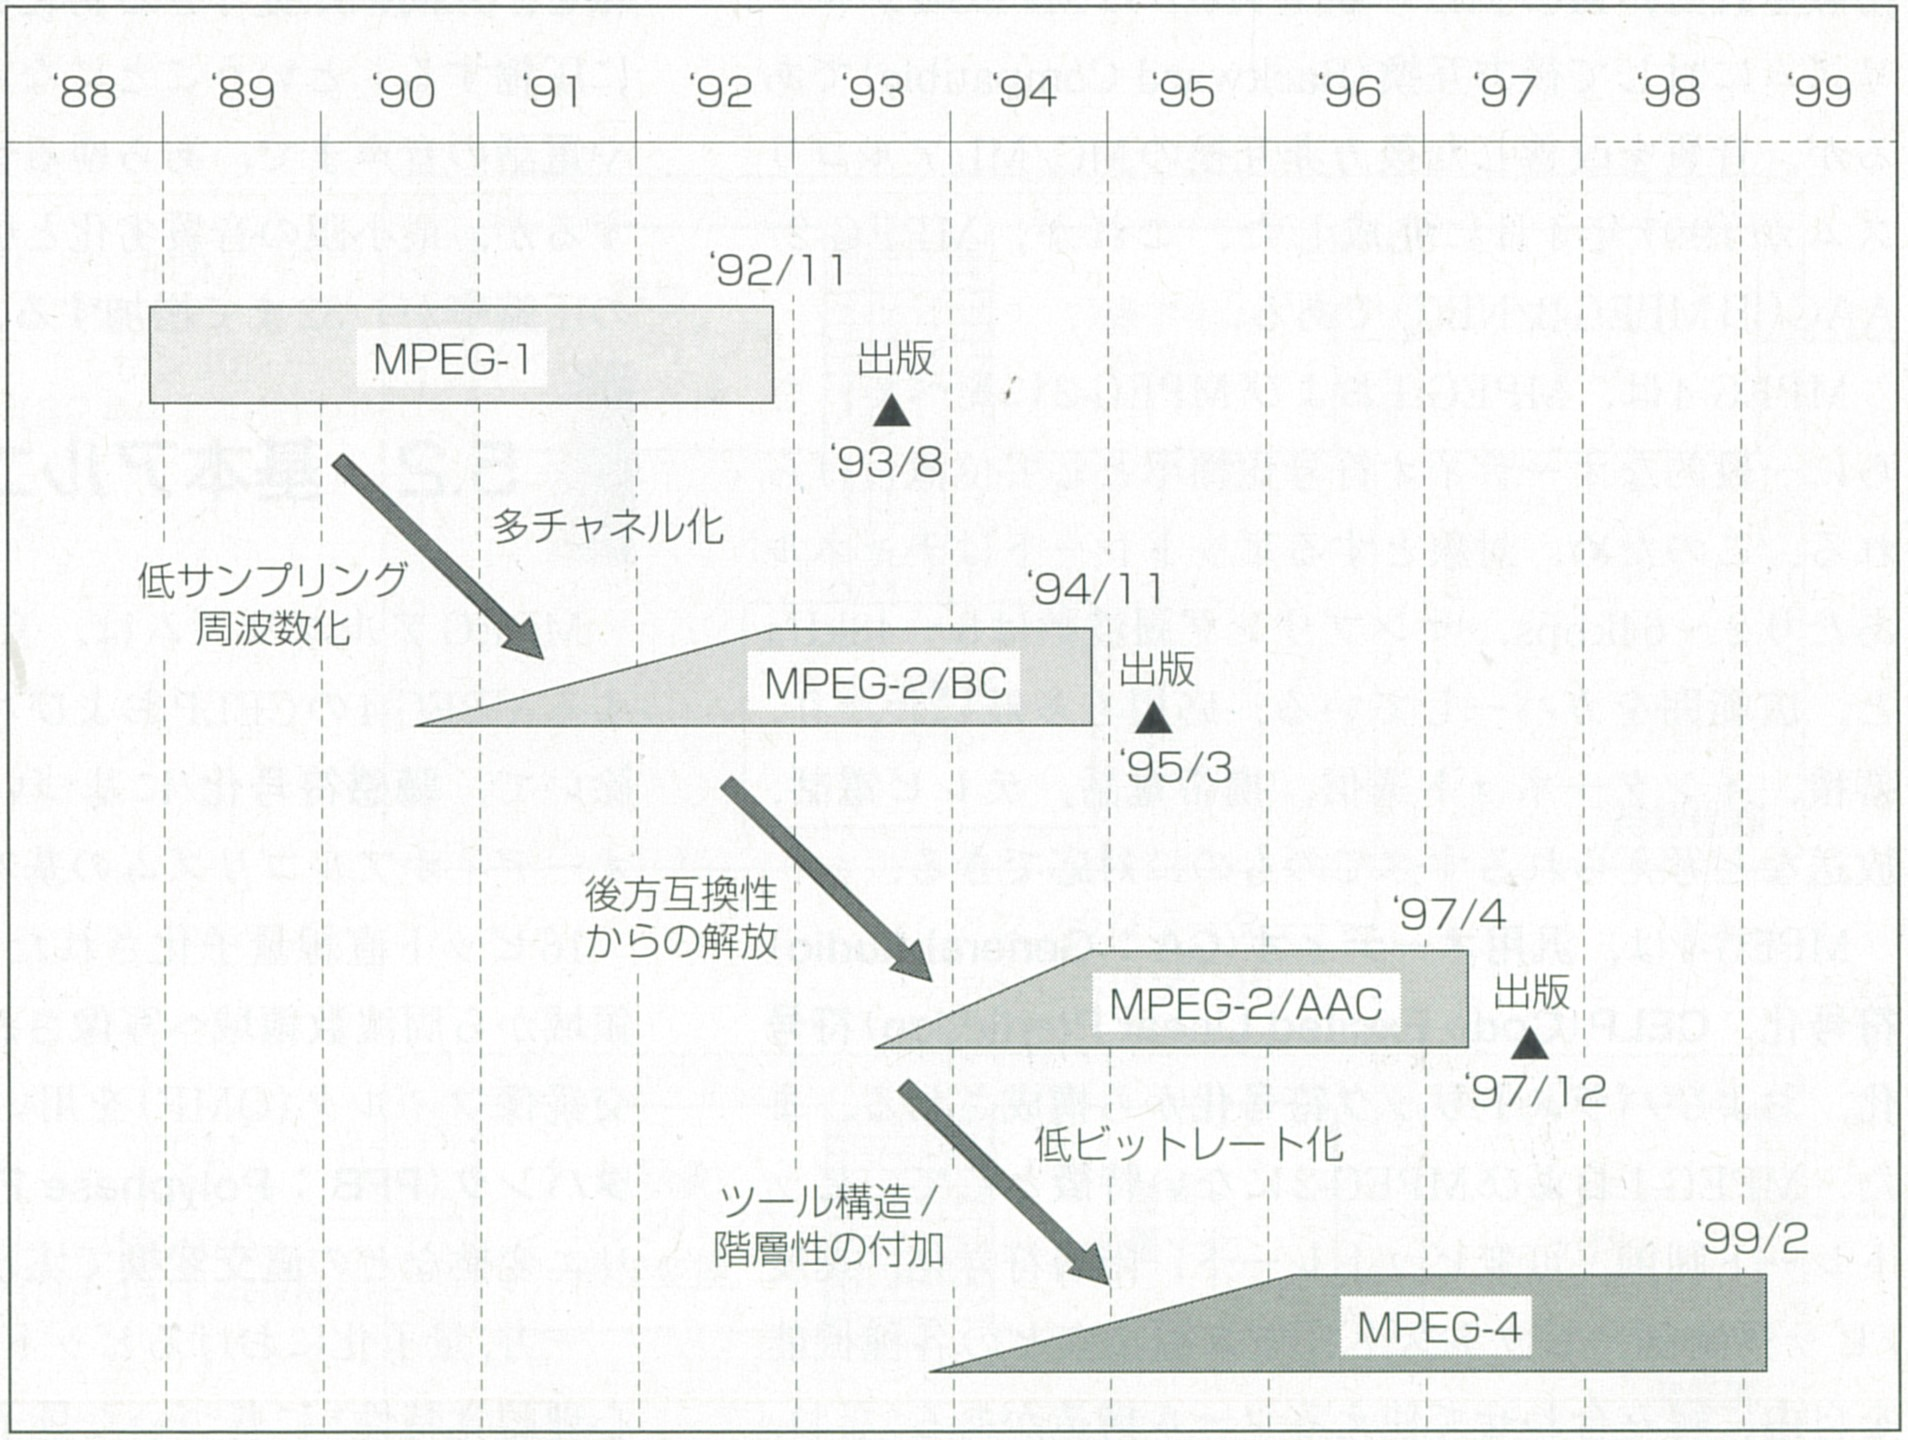
\includegraphics[width=100mm]{./figs/mpeg_history.jpg}
        \caption*{MPEG/Audioの系譜.\cite{fujiwara2001}より引用}
    \end{figure}
\end{frame}

\begin{frame}[c]
    \frametitle{MPEG/Audioの歴史}
    \begin{figure}
        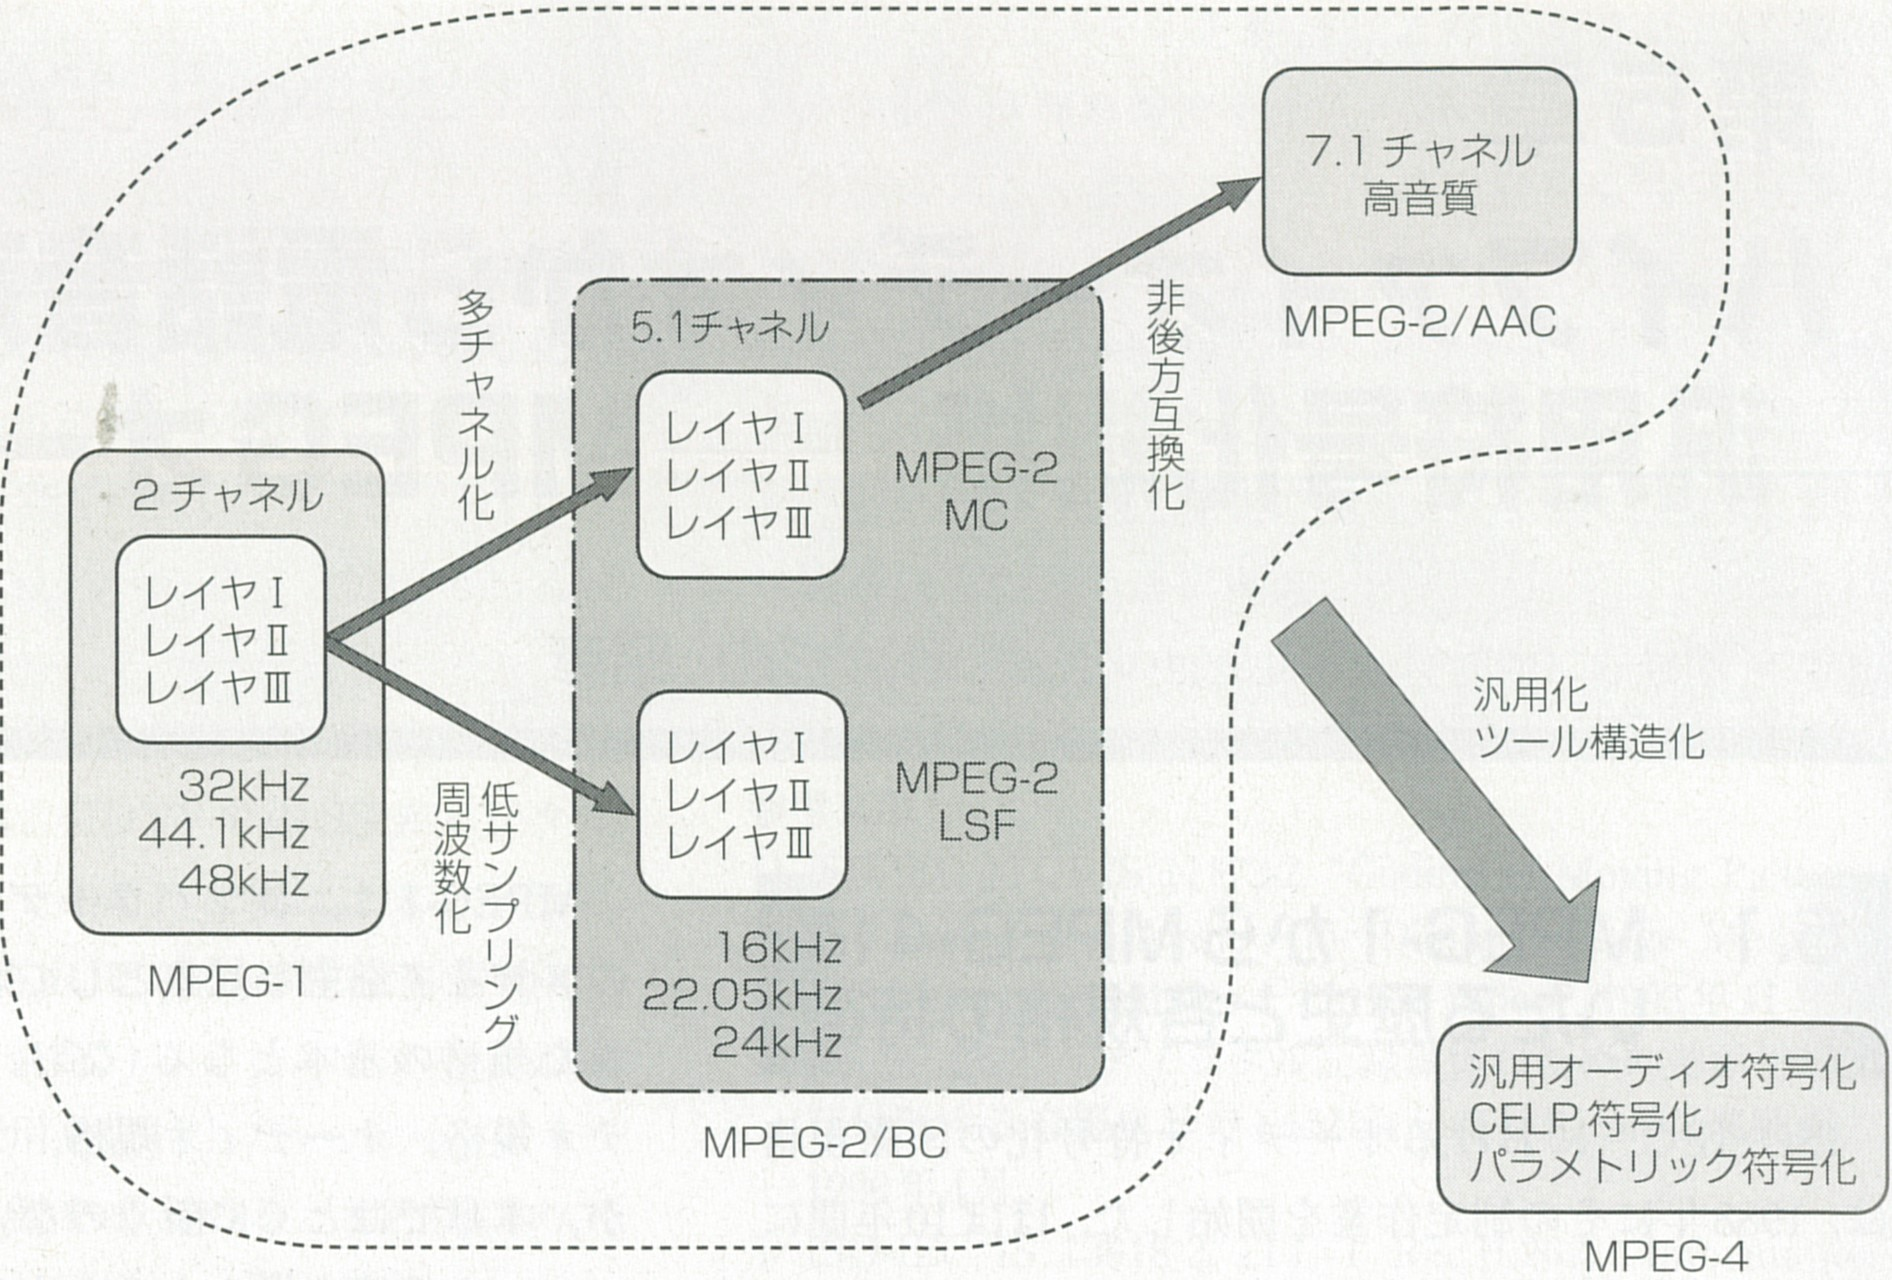
\includegraphics[width=112mm]{./figs/mpeg_relation.jpg}
        \caption*{MPEG/Audioの関係.\cite{fujiwara2001}より引用}
    \end{figure}
\end{frame}

\begin{frame}[c]
    \frametitle{MPEG1の要素技術}
    \begin{columns}
        \begin{column}{0.4\textwidth}
            \begin{itemize}
                \item レイヤI,II,IIIの順に圧縮率向上
                \item レイヤI,IIはサブバンド符号化がメイン
                \item 聴覚心理モデルはI,IIとIIIで異なる
            \end{itemize}
        \end{column}
        \begin{column}{0.6\textwidth}
            \begin{figure}
                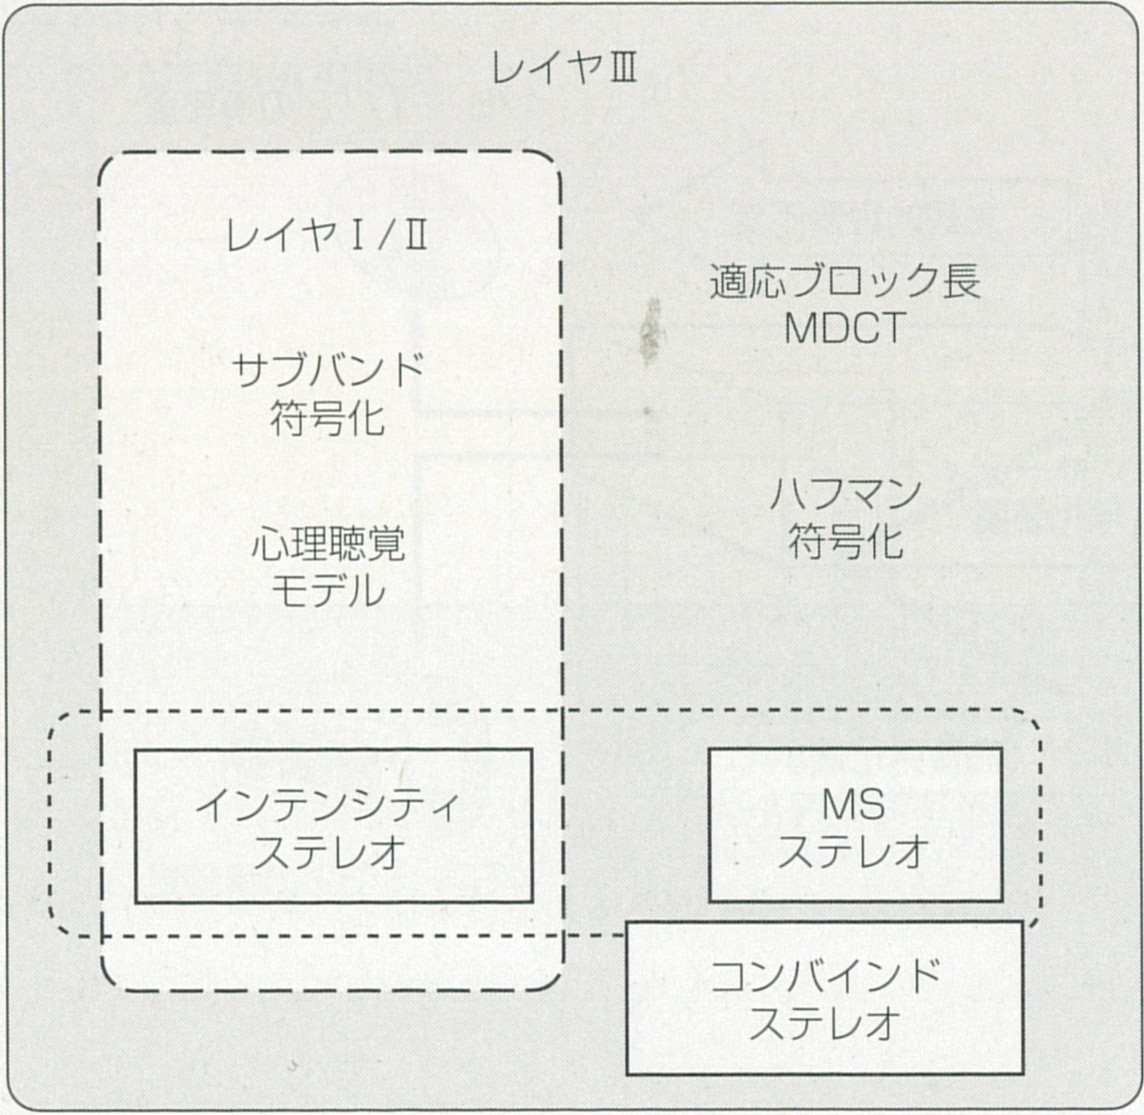
\includegraphics[width=70mm]{./figs/mpeg1_element_technologies.jpg}
                \caption*{\cite{fujiwara2001}より引用}
            \end{figure}
        \end{column}
    \end{columns}
\end{frame}

\subsection{コーデック構造}

\begin{frame}[c]
    \frametitle{MP3のエンコーダ構造}
    \begin{figure}
        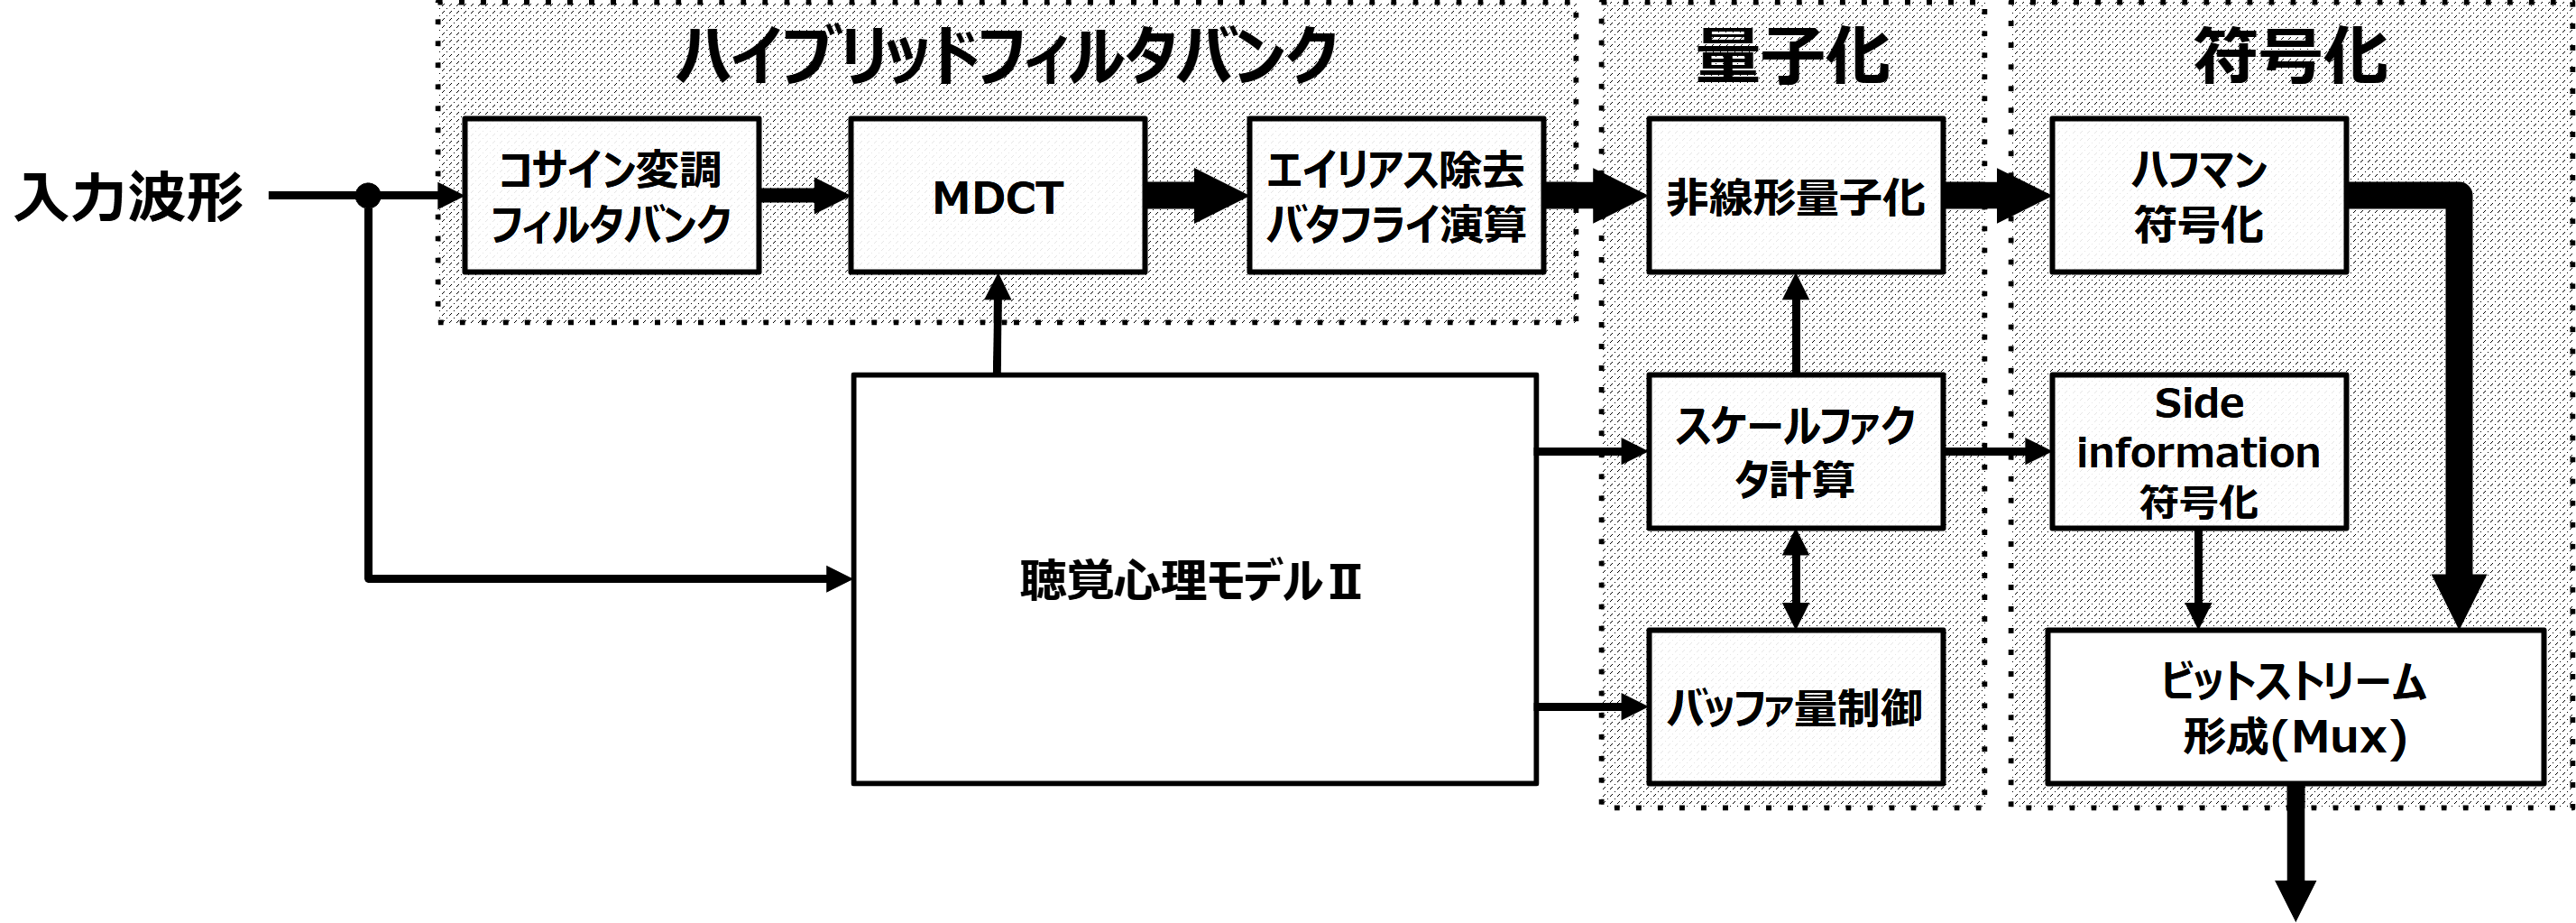
\includegraphics[width=115mm]{./figs/mp3_encoder_struct.png}
    \end{figure}
    \begin{description}
        \item[ハイブリッドフィルタバンク] 32バンドのフィルタバンクの後,18点のMDCT $\rightarrow$ 576点のスペクトルを計算
        \item[量子化] 臨界帯域・マスキングの情報を元にスペクトルを量子化
        \item[符号化] 低域を精密・高域を荒く符号化
    \end{description}
\end{frame}

\begin{frame}[c]
    \frametitle{MP3のデコーダ構造}
    \begin{figure}
        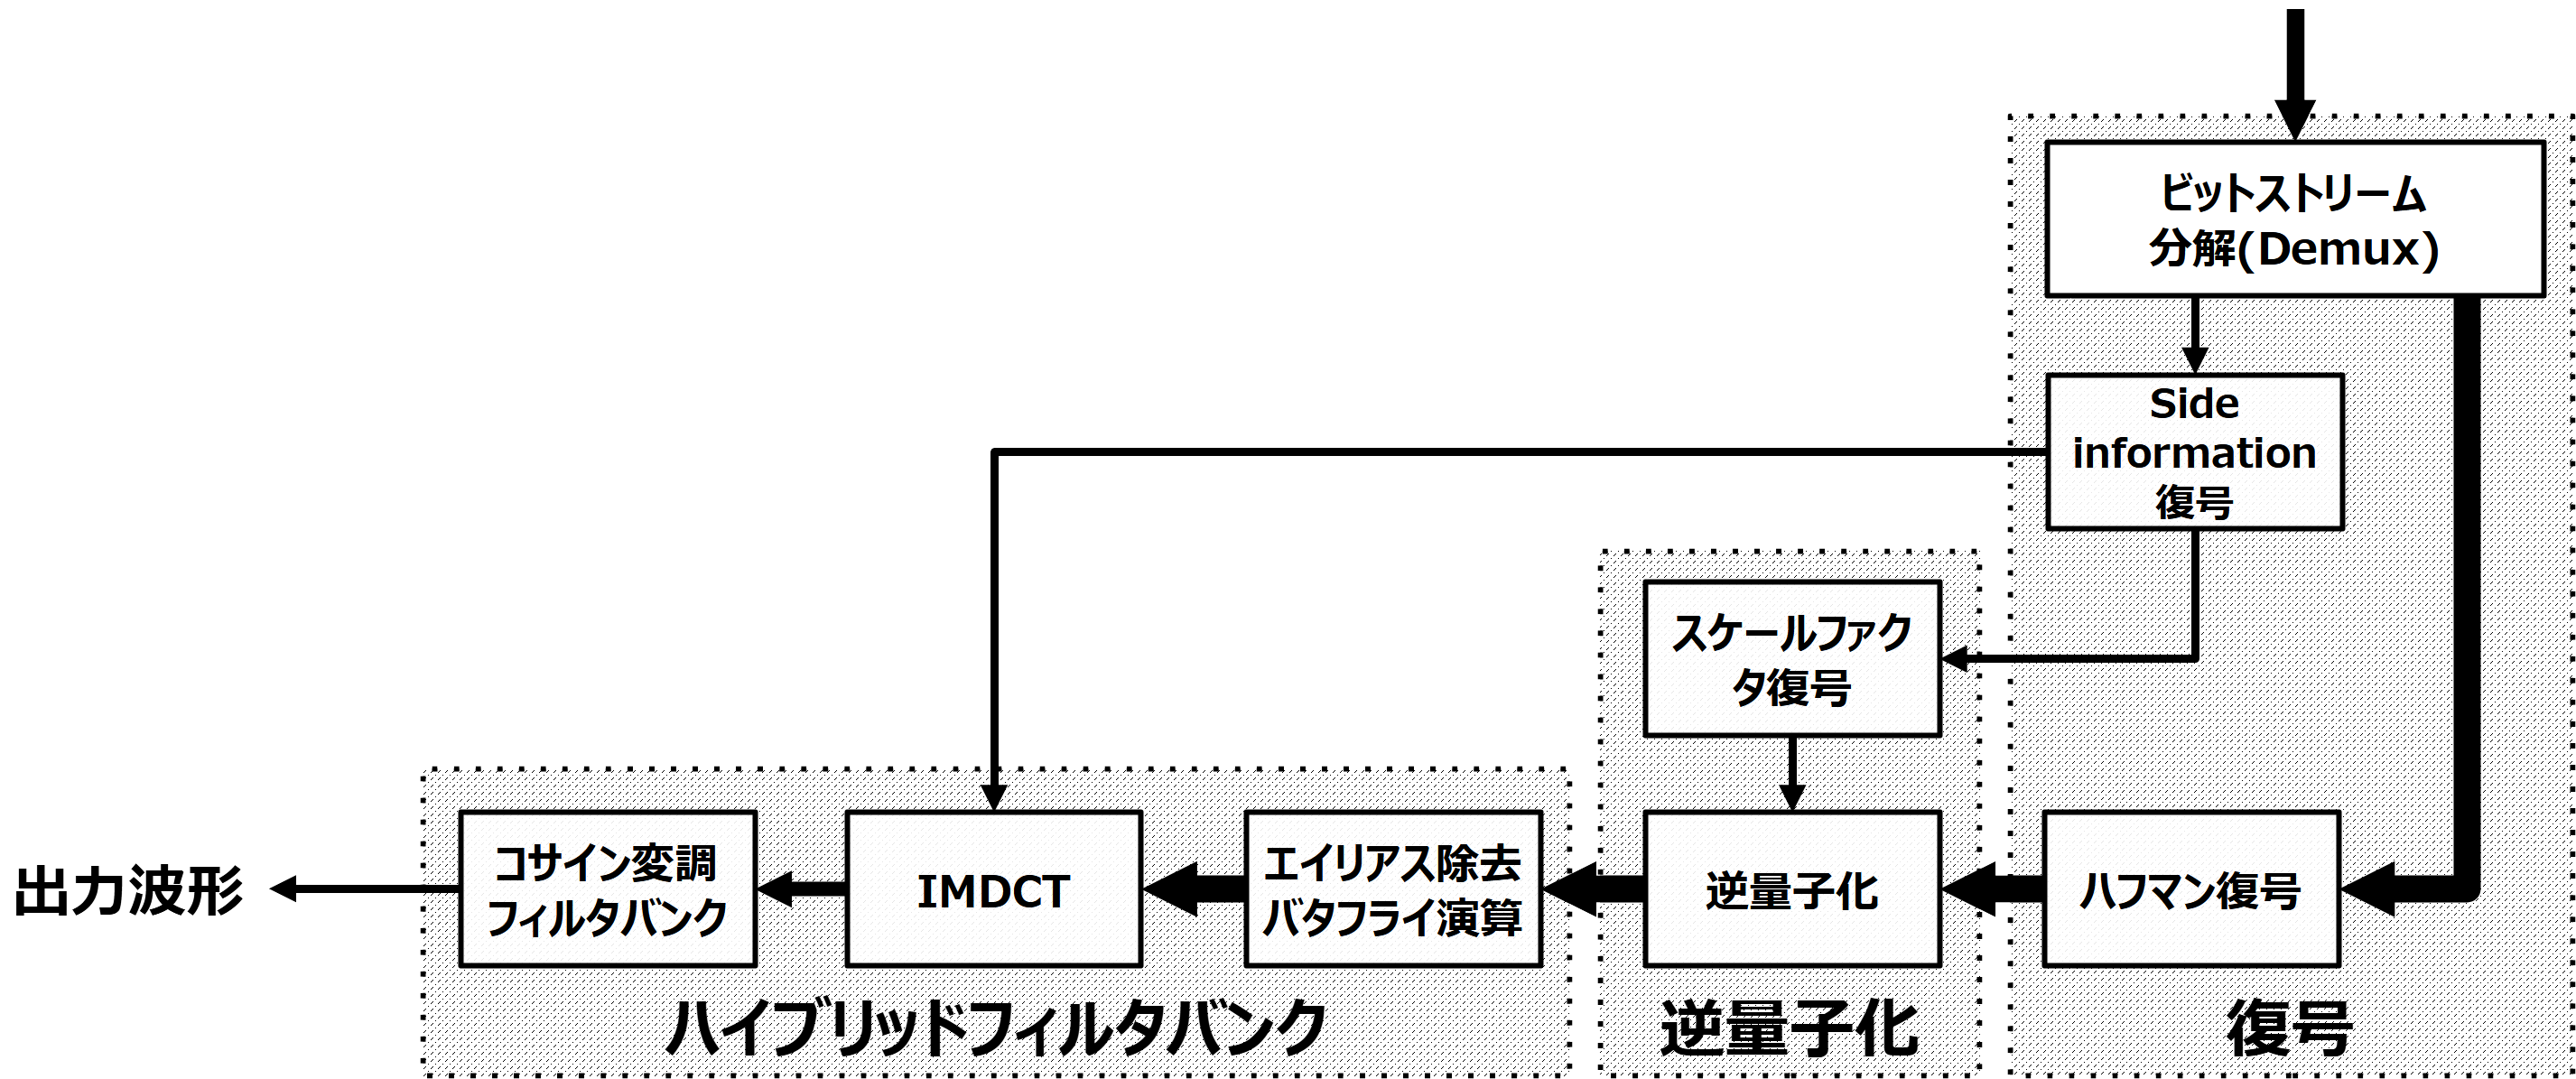
\includegraphics[width=115mm]{./figs/mp3_decoder_struct.png}
    \end{figure}
    エンコーダの逆の操作
\end{frame}

\section{ハイブリッドフィルタバンク}

\subsection{フィルタバンク}

\begin{frame}[c]
    \frametitle{$M$分割フィルタバンク\cite{kiya1995}}
    \begin{figure}
        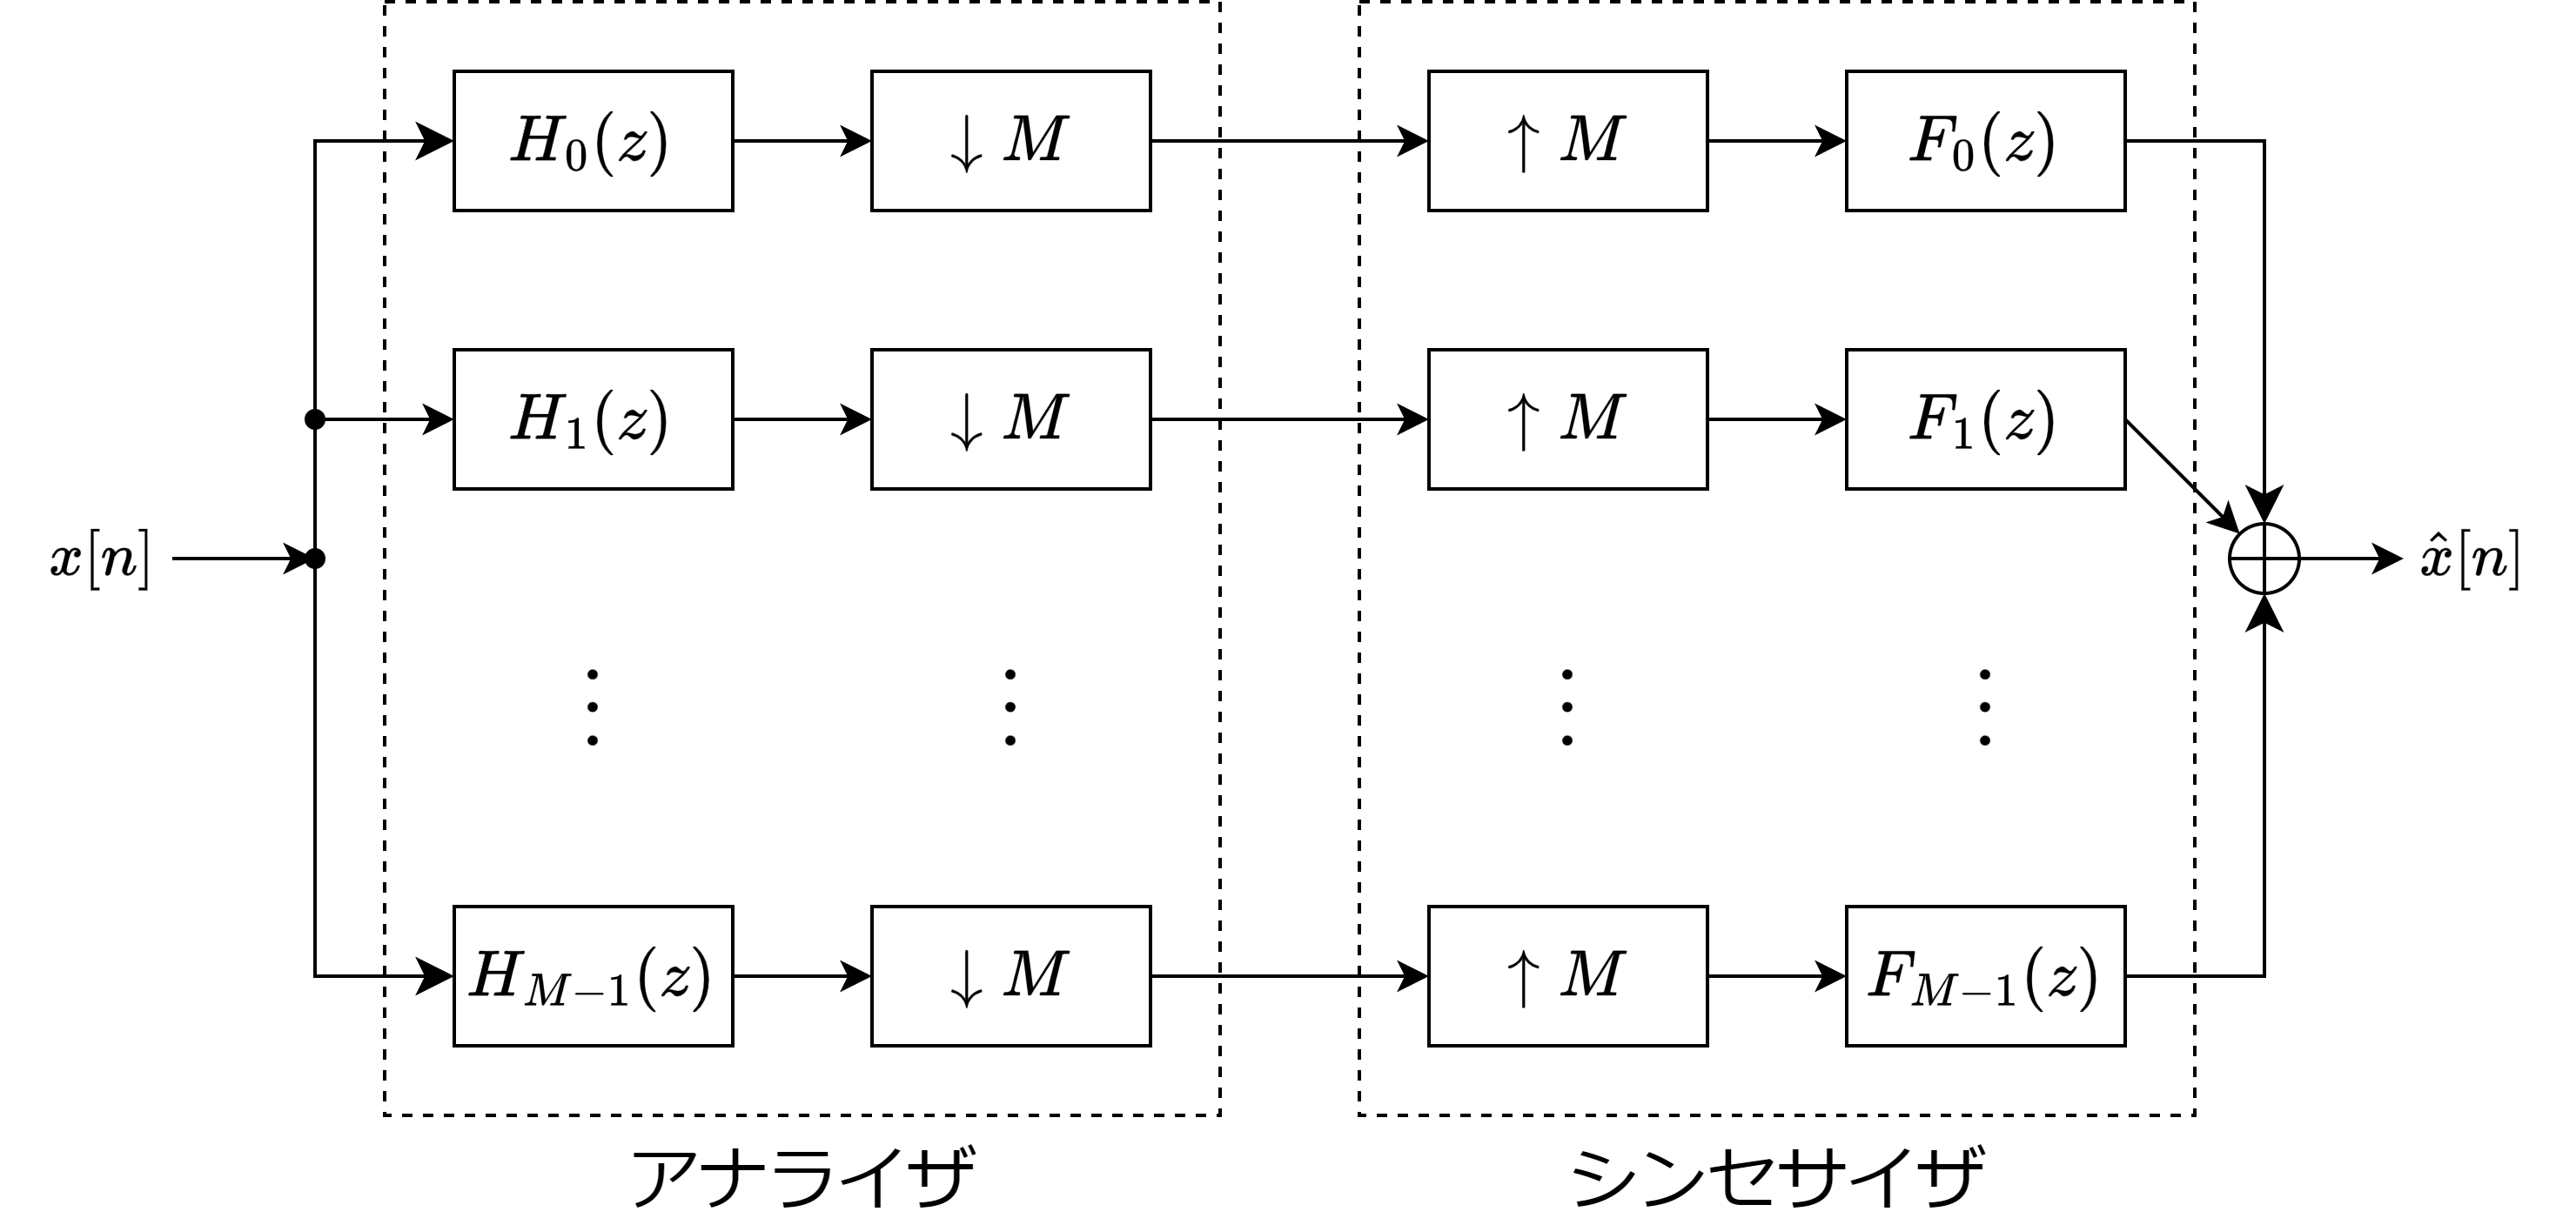
\includegraphics[width=120mm]{./figs/filter_bank.drawio.png}
    \end{figure}
    \begin{itemize}
        \item 信号を$M$個の帯域に分割
        \item $M$個の分析フィルタ$h_{k}$・合成フィルタ$f_{k}$を使用
    \end{itemize}
\end{frame}

\begin{frame}[c]
    \frametitle{コサイン変調フィルタバンク\cite{kiya1995,vaidyanathan2002}}
    \begin{block}{コサイン変調フィルタバンク}
        1つの実係数・直線位相\structure{プロトタイプフィルタ}$p_{0}[n]$から,分析フィルタ$h_{k}$と合成フィルタ$f_{k}$を次で設定:
        \begin{align}
            h_{k}[n] &= 2 p_{0}[n] \cos \left[ \frac{\pi}{M} \left( k + \frac{1}{2} \right) \left( n - \frac{L - 1}{2} \right) + \theta_{k} \right] \label{eq:cos_modulated_analysis_filter} \\
            f_{k}[n] &= h_{k}[L - 1 - n] \label{eq:cos_modulated_synthesis_filter}
        \end{align}
        $M$:分割帯域数,$L$:タップ長,$\theta_{k} = (-1)^{k} \frac{\pi}{4}$
    \end{block}
    詳細は補足\ref{sec:proofs_filter_bank}節に記載
\end{frame}

\begin{frame}[c]
    \frametitle{MP3のフィルタバンク}
    $M = 32, L = 33$としたコサイン変調フィルタバンク\alert{に近いが異なる!($\theta_{k}$がない!)}
    \begin{align}
        h_{k}[n] &= p_{0}[n] \cos\left[ \frac{\pi}{32}\left( k + \frac{1}{2} \right) \left( n - 16 \right) \right] \\
        f_{k}[n] &= 32 p_{0}[n] \cos\left[ \frac{\pi}{32}\left( k + \frac{1}{2} \right) \left( n + 16 \right) \right] \\
        p_{0}[n] &= \left\{ \begin{array}{ll}
            -C_{n} & \lfloor n / 64 \rfloor \text{が偶数} \\
            C_{n} & \lfloor n / 64 \rfloor \text{が奇数} \\
        \end{array} \right.
    \end{align}
    $C_{n}\ (n = 0,...,511)$は規格で設定
\end{frame}

\begin{frame}[c]
    \frametitle{フィルタバンクの特性}
    \vspace{-5pt}
    \begin{figure}
        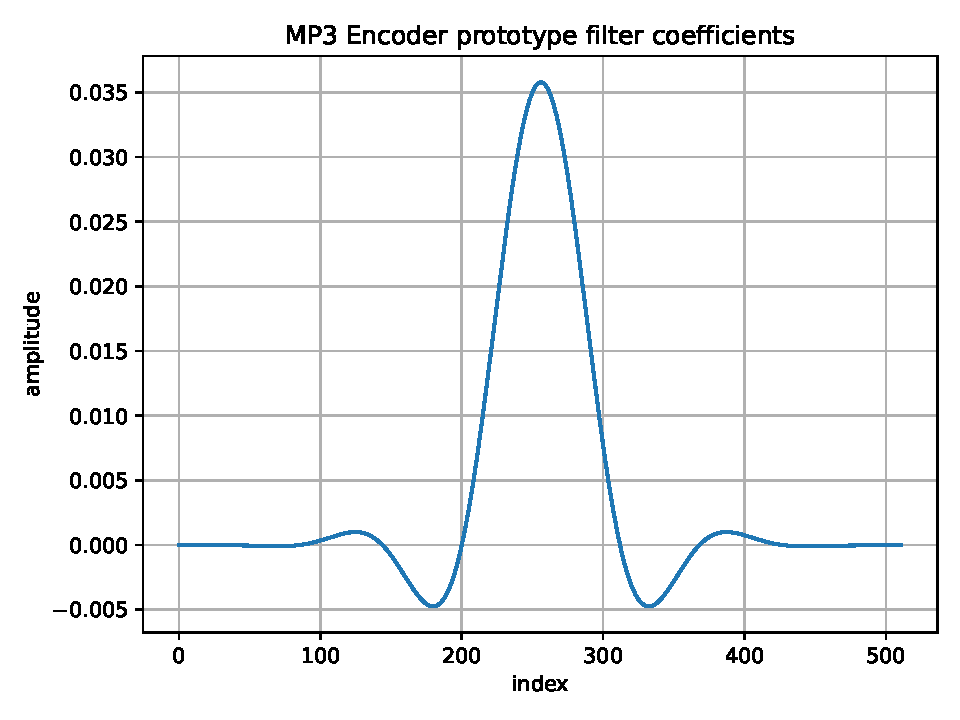
\includegraphics[width=100mm]{./figs/mp3_encoder_prototype_filter_coef.pdf}
    \end{figure}
    \vspace{-5pt}
    \begin{itemize}
        \item $p_{0}[n]$の形状.対称($=$直線位相特性をもつ).
    \end{itemize}
\end{frame}

\begin{frame}[c]
    \frametitle{フィルタバンクの周波数特性}
    バンク$k = 0, ..., 15$の周波数特性
    \vspace{-5pt}
    \begin{figure}
        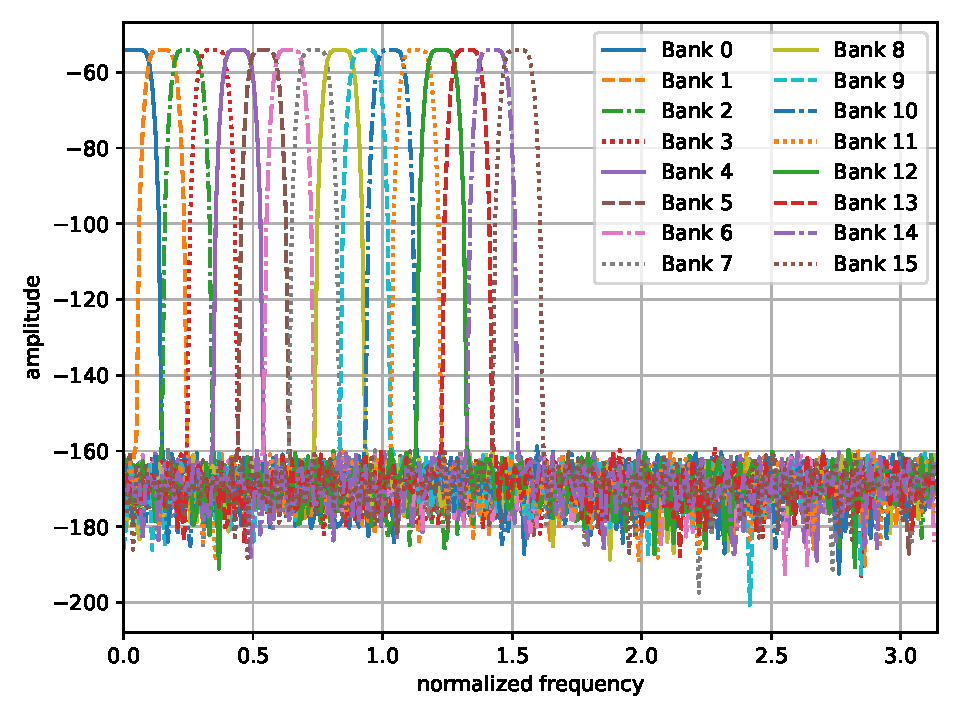
\includegraphics[width=105mm]{./figs/mp3_encoder_filter_bank_frequency_spec_0_15.pdf}
    \end{figure}
\end{frame}

\begin{frame}[c]
    \frametitle{フィルタバンクの周波数特性}
    バンク$k = 16, ..., 31$の周波数特性
    \vspace{-5pt}
    \begin{figure}
        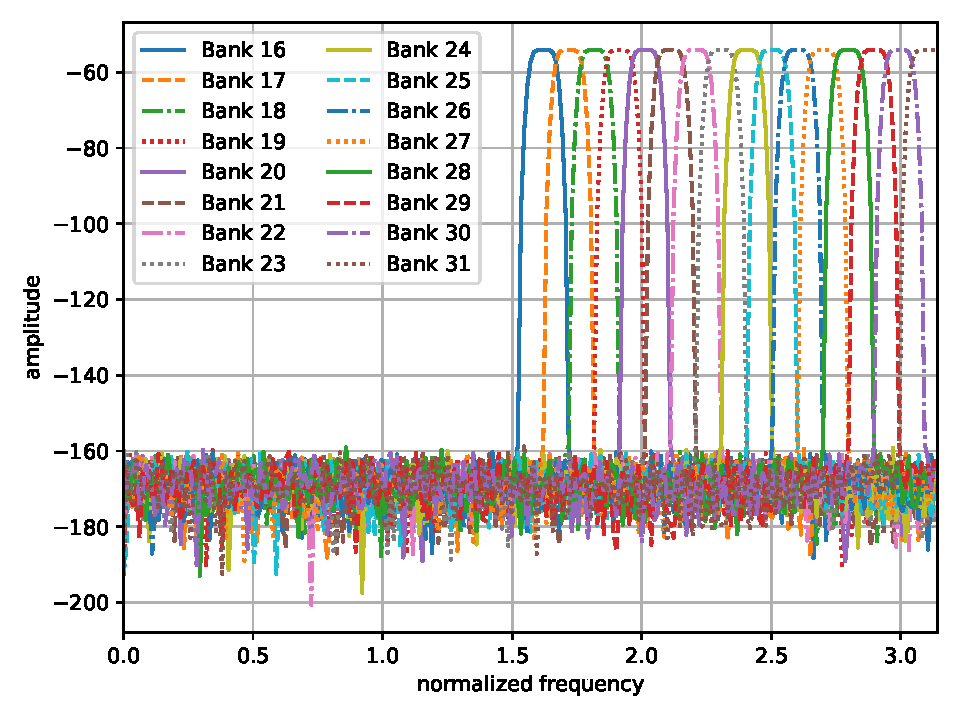
\includegraphics[width=105mm]{./figs/mp3_encoder_filter_bank_frequency_spec_16_31.pdf}
    \end{figure}
\end{frame}

\begin{frame}[c]
    \frametitle{フィルタバンクの実装}
    プログラムでは,入力$x[t]$からバンド$k$の出力$y_{k}[t]$を
    \begin{align*}
        y_{k}[t] &= \sum_{s = 0}^{63} t_{k,s} \sum_{u = 0}^{7} x[t - s - 64u] C_{s + 64u} \\
        t_{k,s} &:= \cos\left[ \frac{\pi}{32}\left( k + \frac{1}{2} \right) \left( s - 16 \right) \right]
    \end{align*}
    で計算.この式がFIRフィルタ出力計算式
    \begin{align}
        y_{k}[t] = \sum_{n = 0}^{511} x[t - n] h_{k}[n] = \sum_{n = 0}^{511} x[t - n] p_{0}[n]  t_{k, n} \label{eq:cos_modulated_filter_fir_output}
    \end{align}
    から導かれることを示す.
\end{frame}

\begin{frame}[c]
    \frametitle{フィルタバンクの実装}
    \scriptsize
    \eqref{eq:cos_modulated_filter_fir_output}式を変形していくと,
    \begin{align}
        y_{k}[t] &= \sum_{n = 0}^{511} x[t - n] p_{0}[n] t_{k, n} = \sum_{u = 0}^{7} \sum_{s = 0}^{63} x[t - s - 64u] p_{0}[s + 64u] t_{k,s+64u} \nonumber \\
        &= \sum_{u = 0}^{7} \sum_{s = 0}^{63} x[t - s - 64u] (-1)^{u} C_{s + 64u} t_{k,s+64u} \label{eq:mp3_filterbank_progaram_deviation}
    \end{align}
    ここで,
    \begin{align*}
        t_{k,s+64u} &= \cos\left[ \frac{\pi}{32} \left( k + \frac{1}{2} \right) (s + 64u - 16) \right] = \cos\left[ \frac{\pi}{32} \left( k + \frac{1}{2} \right) (s - 16) + \pi \left( 2k + 1 \right) u \right] \\
        &= \cos\left[ \frac{\pi}{32} \left( k + \frac{1}{2} \right) (s - 16) \right]\cos\left[ \pi(2k + 1)u \right] \\
        &\quad - \sin\left[ \frac{\pi}{32} \left( k + \frac{1}{2} \right) (s - 16) \right]\sin\left[ \pi(2k + 1)u \right]
        % &= (-1)^{u} \cos\left[ \frac{\pi}{32} \left( k + \frac{1}{2} \right) (s - 16) \right] = (-1)^{u}
        = (-1)^{u} t_{k,s}
    \end{align*}
    だから,これを式\eqref{eq:mp3_filterbank_progaram_deviation}に代入すれば,
    \begin{align*}
        y_{k}[t] = \sum_{u = 0}^{7} \sum_{s = 0}^{63} x[t - s - 64u] C_{s + 64u} t_{k,s} = \sum_{s = 0}^{63} t_{k,s} \sum_{u = 0}^{7} x[t - s - 64u] C_{s + 64u}
    \end{align*}
    プログラムの計算式が導かれた.
\end{frame}

\begin{frame}[c]
    \frametitle{フィルタバンクは完全再構成か?}
    \begin{itemize}
        \item $C_{n}$の導出方法が不明.厳密に完全再構成性を示せない
        \item 再構成信号$\hat{x}[n]$が入力信号の遅延+定数倍になるか観察
            \small
            \begin{align*}
                \left\{ \begin{array}{ll}
                    y_{k}[n] = \displaystyle\sum_{i = 0}^{511} h_{k}[i] x[n - i] & \text{バンク$k$の分析フィルタ出力} \\
                    z_{k}[n] = \displaystyle\sum_{i = 0}^{511} f_{k}[i] y_{k}[n - i] & \text{バンク$k$の合成フィルタ出力} \\
                    \hat{x}[n] = \displaystyle\sum_{k = 0}^{31} z_{k}[n] & \text{再構成信号}
                \end{array} \right.
            \end{align*}
    \end{itemize}
\end{frame}

\begin{frame}[c]
    \frametitle{フィルタバンクは完全再構成か?}
    \small
    \vspace{-10pt}
    \begin{align}
        \hat{x}[n] &= \sum_{k = 0}^{31} z_{k}[n] = \sum_{k = 0}^{31} \left( \sum_{i = 0}^{511} f_{k}[i] y_{k}[n - i] \right) \nonumber \\
        &= \sum_{k = 0}^{31} \left\{ \sum_{i = 0}^{511} f_{k}[i] \left( \sum_{j = 0}^{511} h_{k}[j] x[n - i - j] \right) \right\} \nonumber \\
        &= \sum_{k = 0}^{31} \sum_{i = 0}^{511} \sum_{j = 0}^{511} f_{k}[i] h_{k}[j] x[n - i - j] \nonumber \\
        &= \sum_{k = 0}^{31} \sum_{m = 0}^{1022} \sum_{i = \max\{ 0, m-511 \}}^{\min\{ 511, m \}} f_{k}[i] h_{k}[m - i] x[n - m] \quad (m := i + j) \nonumber \\
        &= \sum_{m = 0}^{1022} x[n - m] \underbrace{\sum_{i = \max\{ 0, m-511 \}}^{\min\{ 511, m \}} \sum_{k = 0}^{31} f_{k}[i] h_{k}[m - i]}_{=g[m]}
    \end{align}
\end{frame}

\begin{frame}[c]
    \frametitle{フィルタバンクは完全再構成か?}
    \begin{columns}
        \begin{column}{0.475\textwidth}
            \begin{itemize}
                \item $g[m]$のグラフ(右図)
                \item $g[m] \approx 32\delta_{m,512}$だから,
                    \begin{align*}
                        \hat{x}[n] \approx 32 x[n - 512]
                    \end{align*}
                    \structure{近似的に完全再構成}
            \end{itemize}
        \end{column}
        \begin{column}{0.65\textwidth}
            \vspace*{-13pt}
            \begin{figure}
                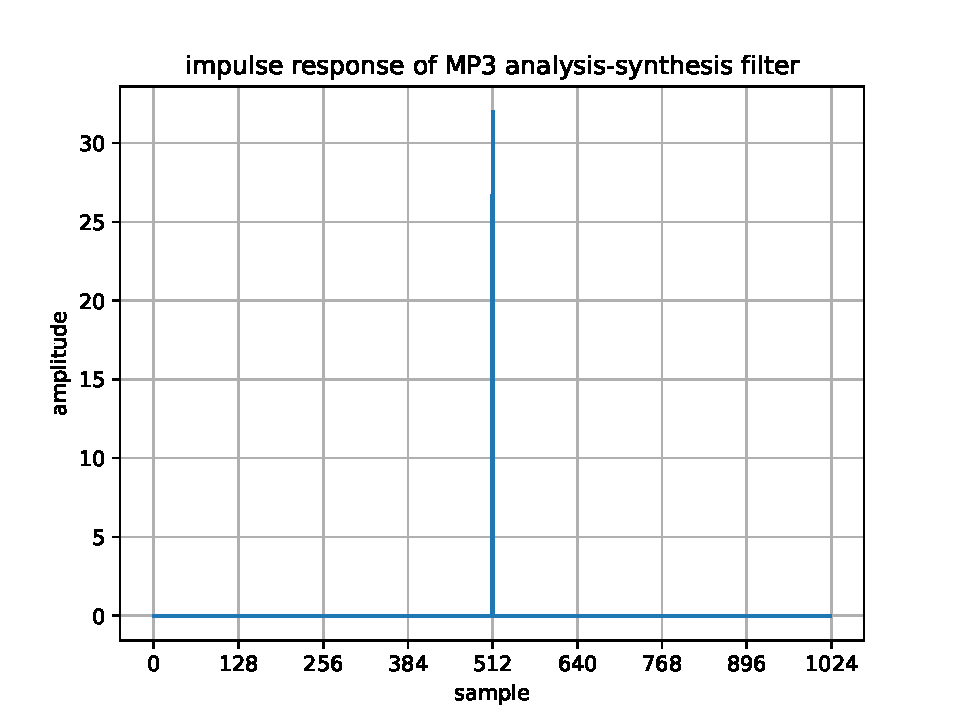
\includegraphics[width=65mm]{./figs/impluse_responce_of_MP3_analysis_synthesis_filter.pdf}
            \end{figure}
        \end{column}
    \end{columns}
\end{frame}

\subsection{MDCT (Modified Discrete Cosine Transform)}

\begin{frame}[c]
    \frametitle{MP3のMDCT (Modified DCT)}
    \begin{itemize}
        \item サブバンドフィルタで32帯域に分割した信号に対し,18点MDCTを実行
            \begin{itemize}
                \item 出力:$32 \times 18 = 576$点のスペクトルデータ
            \end{itemize}
        \item MDCTの前・IMDCTの後で窓関数を適用
            \begin{itemize}
                \item MP3では4種類の窓関数を使用
                \item 窓関数は完全再構成条件を満たす
            \end{itemize}
    \end{itemize}
\end{frame}

\begin{frame}[c]
    \frametitle{MDCTとIMDCT}
    入力信号を$x[n]$,再構成信号を$y[n]$として
    \begin{block}{MDCT (Modified Discrete Cosine Transform)}
        \vspace{-15pt}
        \begin{align}
            X_{k} = \sum_{n = 0}^{2N - 1} x[n] \cos\left[ \frac{\pi}{N} \left( k + \frac{1}{2} \right) \left( n + \frac{1}{2} + \frac{N}{2} \right) \right] \label{eq:mdct}
        \end{align}
    \end{block}
    \begin{block}{IMDCT (Inverse MDCT)}
        \vspace{-15pt}
        \begin{align}
            y[n] = \frac{2}{N} \sum_{k = 0}^{N - 1} X_{k} \cos\left[ \frac{\pi}{N} \left( k + \frac{1}{2} \right) \left( n + \frac{1}{2} + \frac{N}{2} \right) \right] \label{eq:imdct}
        \end{align}
    \end{block}
    \begin{itemize}
        \item 時間領域は$2N$点,周波数領域は$N$点の変換($k = 0, ..., N-1$)
    \end{itemize}
\end{frame}

\begin{frame}[c]
    \frametitle{MDCTと完全再構成条件}
    \eqref{eq:imdct}式に\eqref{eq:mdct}式を代入して整理すると
    \begin{align}
        y[n] =
        \left\{ \begin{array}{ll}
            x[n] - x[N - 1 - n] & (n = 0, ..., N - 1) \\
            x[n] + x[3N - 1 - n] & (n = N, ..., 2N - 1)
        \end{array} \right. \label{eq:mdct_reconstruction}
    \end{align}
    となる(証明は補足).
    \begin{block}{}
        \structure{ハーフオーバーラップで処理するとき,$x[n], y[n]$にうまく窓関数を適用すると完全再構成にできる.}その条件は?
    \end{block}
\end{frame}

\begin{frame}[c]
    \frametitle{ハーフオーバーラップアドの手順}
    \vspace*{-25pt}
    \begin{columns}
        \begin{column}{0.5\textwidth}
            \vspace*{12pt}
            \begin{figure}
                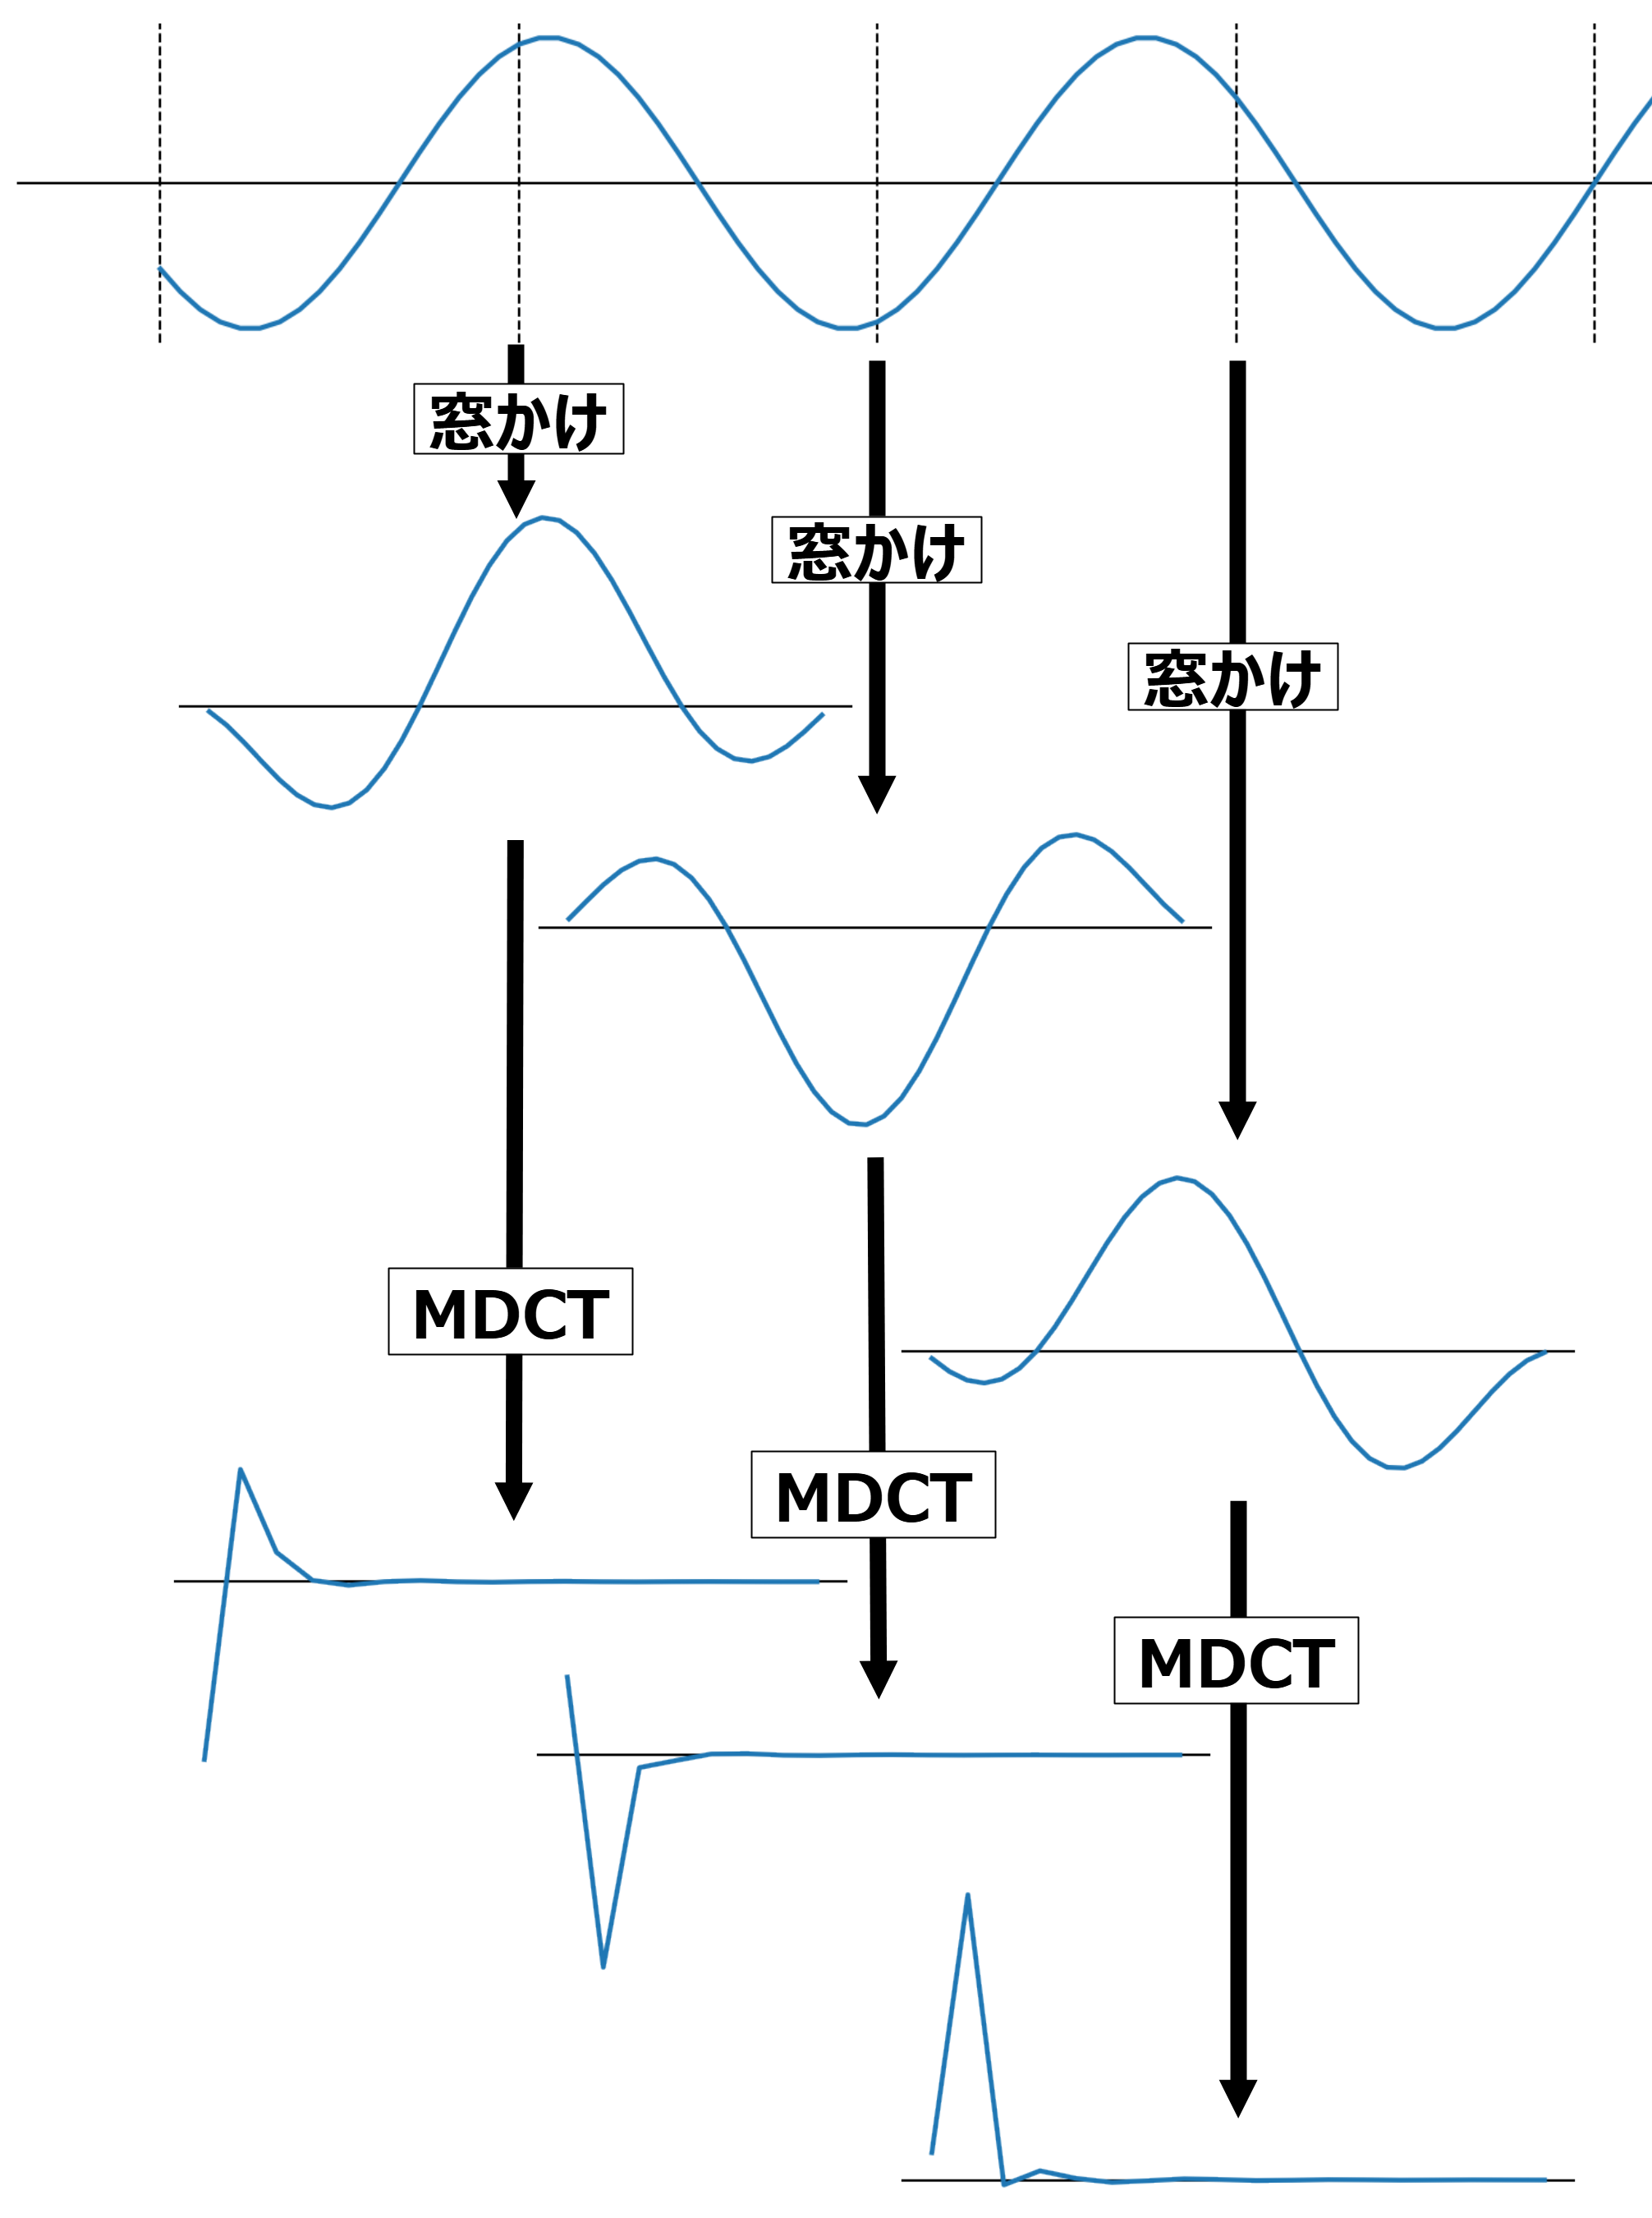
\includegraphics[width=58mm]{./figs/halft_overlap_add_encode.png}
                \caption*{エンコード}
            \end{figure}
        \end{column}
        \begin{column}{.01\textwidth}
            % \rule{.5mm}{.7\textheight}
            \vspace*{60pt}
            \rotatebox{-90}{\hskip-1.8cm\hdashrule[0.2ex]{8cm}{1pt}{3mm}}
        \end{column}
        \hspace{-10pt}
        \begin{column}{0.5\textwidth}
            \vspace*{12pt}
            \begin{figure}
                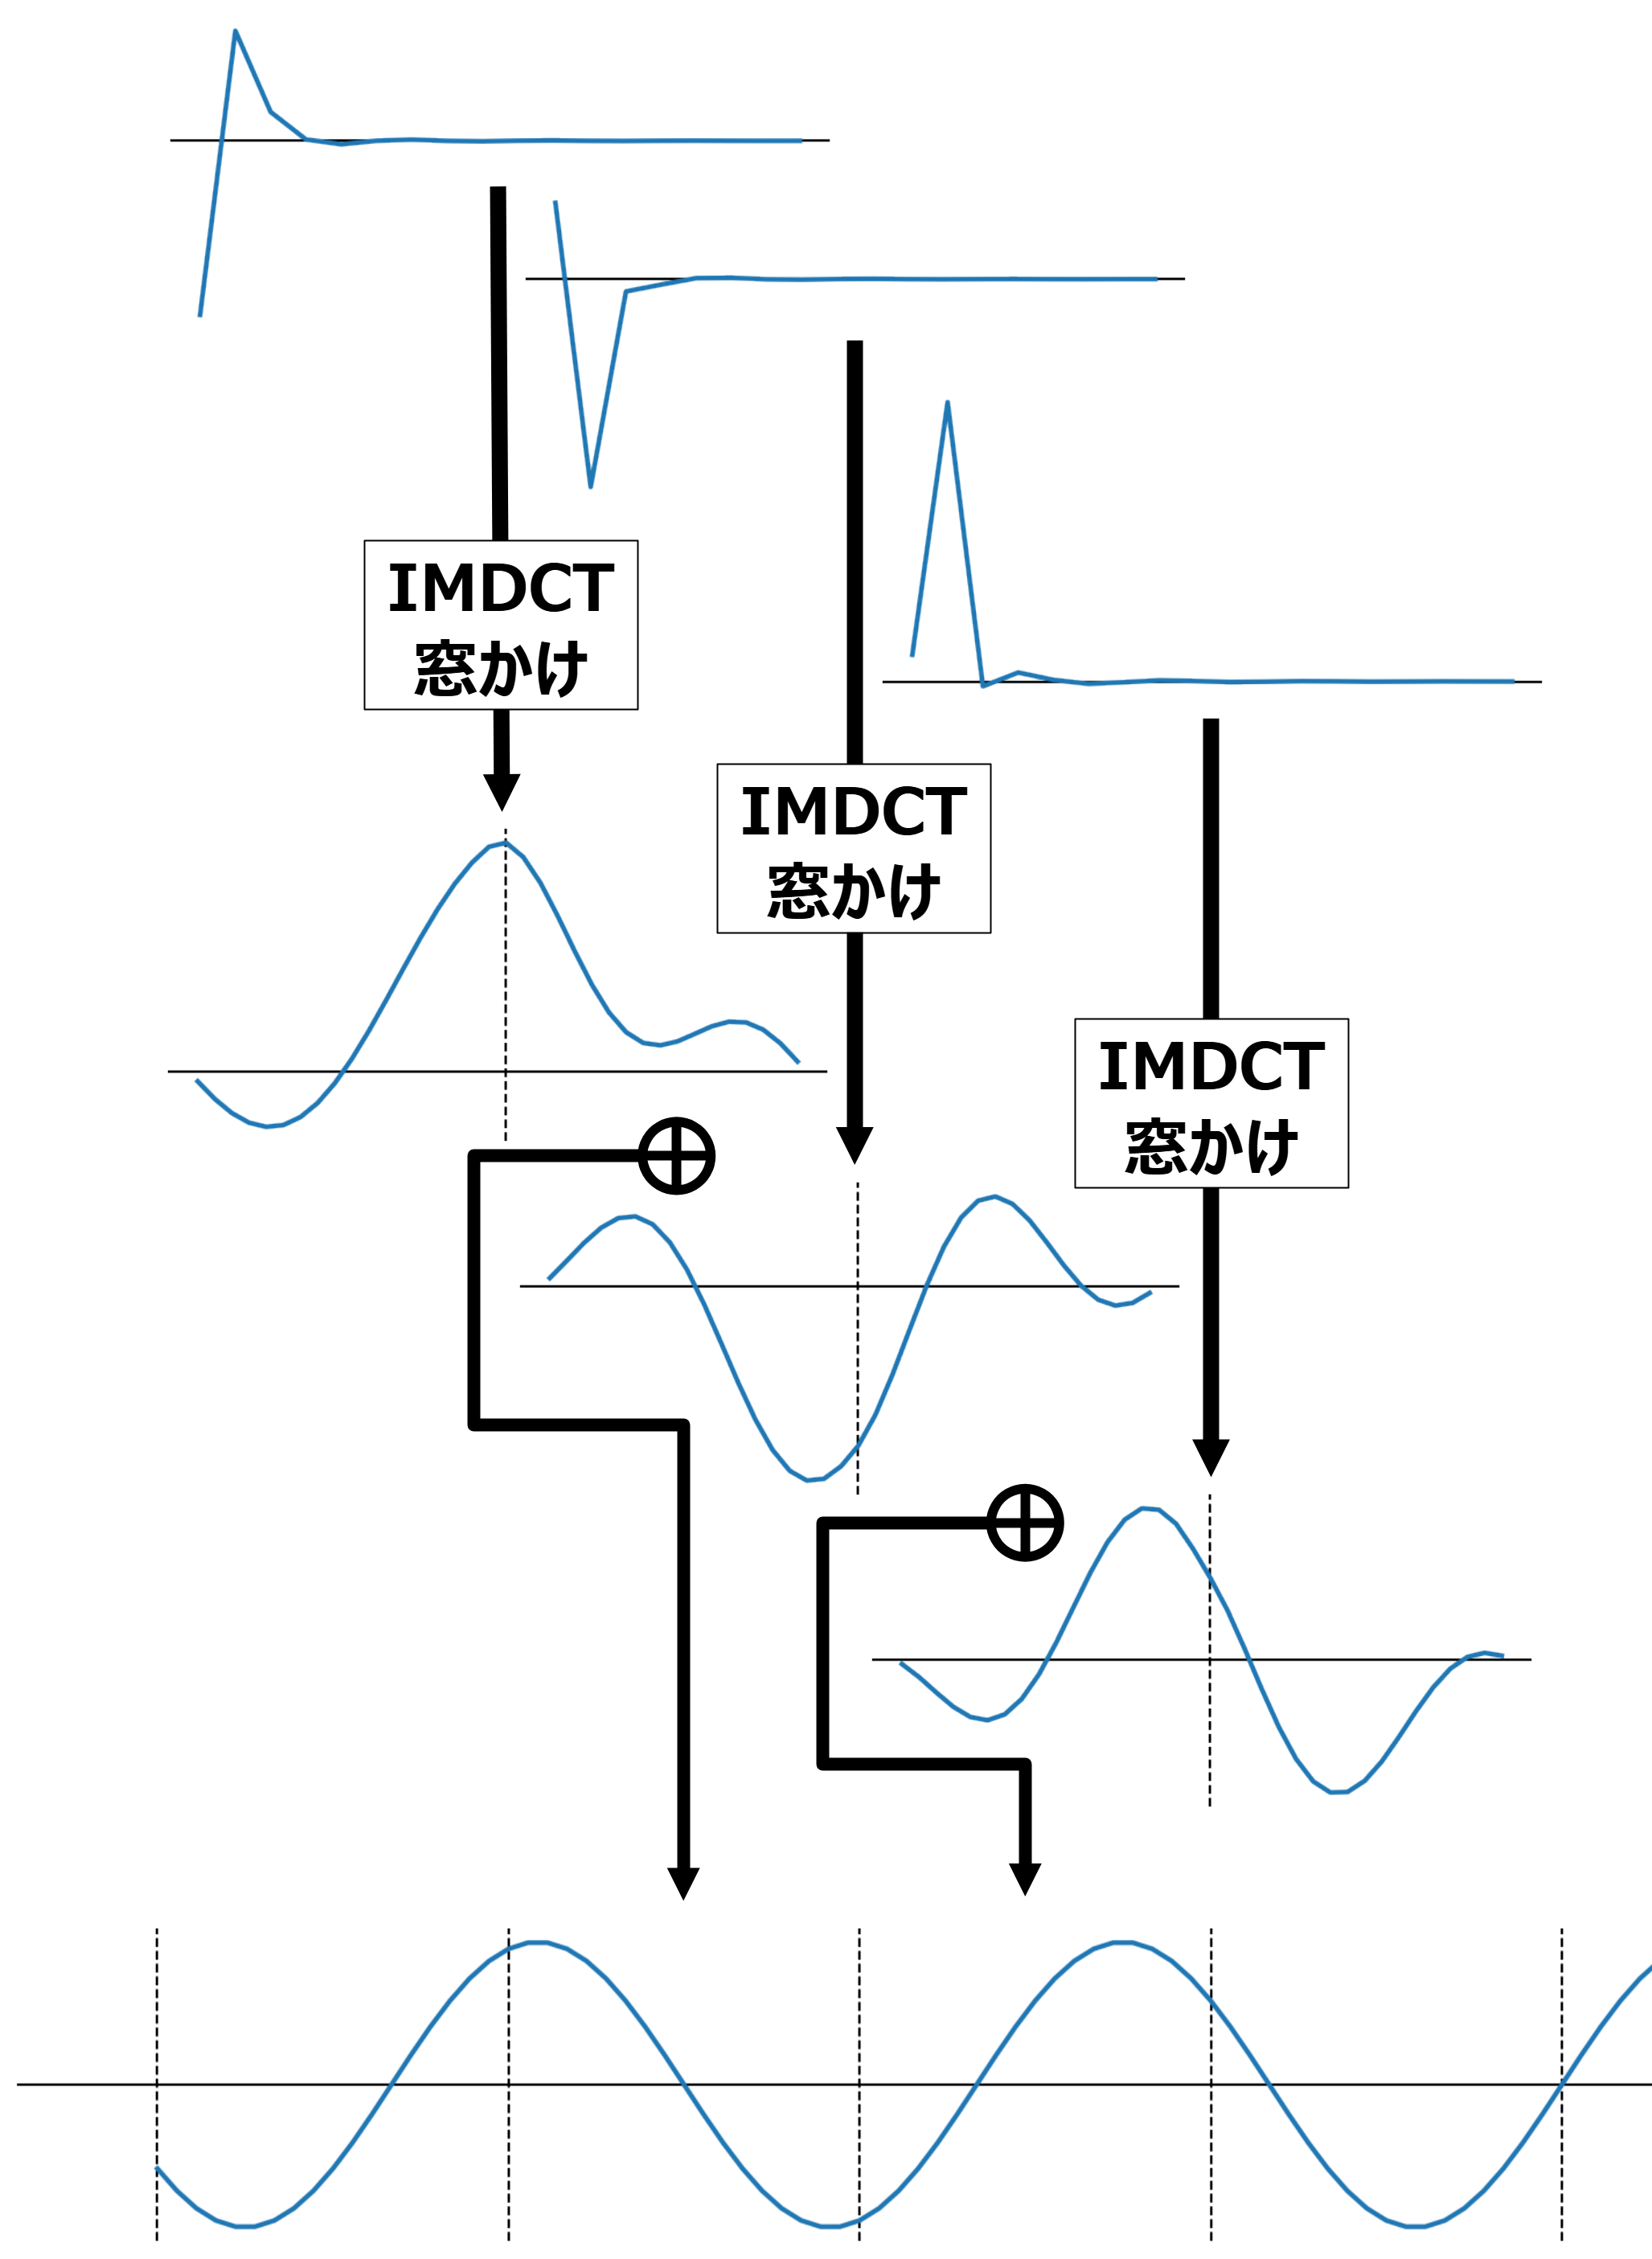
\includegraphics[width=57mm]{./figs/halft_overlap_add_decode.png}
                \caption*{デコード}
            \end{figure}
        \end{column}
    \end{columns}
\end{frame}

\begin{frame}[c]
    \frametitle{MDCTと完全再構成条件}
    \begin{block}{Princen--Bradley条件(完全再構成条件)\cite{princen1986analysis}}
        長さ$2N$の分析窓を$w_{a}$,合成窓を$w_{s}$としたとき,
        \begin{align}
            w_{a}[n] w_{s}[n] + w_{a}[n + N]w_{s}[n + N] = 1 & \label{eq:princen_bradley_conditon_1} \\
            w_{a}[n + N] w_{s}[2N - 1 - n] = w_{a}[n]w_{s}[N - 1 - n] & \label{eq:princen_bradley_conditon_2} \\
            n = 0,...,N-1 & \nonumber
        \end{align}
        ならば,MDCT・IMDCTによるハーフオーバーラップアドは完全再構成
    \end{block}
\end{frame}

\begin{frame}[c]
    \frametitle{Princen--Bradley条件の導出}
    % TODO: g, zなど中間変数が多い。減らしたい
    $m$フレーム目の$n$時刻の入力$x_{m}[n]$は,フレームあたり$N$サンプルでスライドしており
    \begin{align}
        x_{m}[n] = x_{m - 1}[n + N]
    \end{align}
    が成り立つとする.窓かけした信号$g_{m}[n]$を
    \begin{align}
        g_{m}[n] := w_{a}[n] x_{m}[n] \quad (n = 0, ..., 2N-1)
    \end{align}
    と書く.$g_{m}[n]$をMDCT・IMDCTして再構成した信号$z_{m}[n]$は,\eqref{eq:mdct_reconstruction}式より,
    \small
    \begin{align}
        z_{m}[n] = \left\{ \begin{array}{ll}
            g_{m}[n] - g_{m}[N - 1 - n] & (n = 0, ..., N - 1) \\
            g_{m}[n] + g_{m}[3N - 1 - n] & (n = N, ..., 2N - 1)
        \end{array} \right. \label{eq:windowed_mdct_reconstruction}
    \end{align}
\end{frame}

\begin{frame}[c]
    \frametitle{Princen--Bradley条件の導出}
    ハーフオーバーラップアドした結果を$\hat{x}_{m}[n]$と書くと,\eqref{eq:windowed_mdct_reconstruction}式より,
    \footnotesize
    \begin{align*}
        &\hat{x}_{m}[n] = w_{s}[n]z_{m}[n] + w_{s}[n + N]z_{m-1}[n + N] \\
        &= w_{s}[n] (g_{m}[n] - g_{m}[N - 1 - n]) \\
        &\quad + w_{s}[n + N] (g_{m-1}[n + N] + g_{m-1}[3N - 1 - (n + N)]) \\
        &= w_{s}[n] (w_{a}[n] x_{m}[n] - w_{a}[N - 1 - n]x_{m}[N - 1 - n]) \\
        &\quad + w_{s}[n + N] (w_{a}[n + N] x_{m-1}[n + N] + w_{a}[2N - 1 - n]x_{m-1}[2N - 1 - n]) \\
        &= w_{s}[n] (w_{a}[n] x_{m}[n] - w_{a}[N - 1 - n]x_{m}[N - 1 - n]) \\
        &\quad + w_{s}[n + N] (w_{a}[n + N] x_{m}[n] + w_{a}[2N - 1 - n]x_{m}[N - 1 - n]) \\
        &= x_{m}[n](w_{a}[n] w_{s}[n] + w_{a}[n + N]w_{s}[n + N]) \\
        &\quad + x_{m}[N - 1 - n](w_{a}[n + N] w_{s}[2N - 1 - n] - w_{a}[n]w_{s}[N - 1 - n])
    \end{align*}
    \normalsize
    この結果を$x_{m}[n] = \hat{x}_{m}[n]$として両辺比較することで条件が得られる
\end{frame}

\begin{frame}[c]
    \frametitle{MP3とPrincen--Bradley条件}
    \begin{block}{Princen--Bradley条件(分析窓と合成窓が同一)}
        分析・合成窓が同じ$w[n] = w_{a}[n] = w_{s}[n]$とき,
        \begin{align}
            w[n]^{2} + w[n + N]^{2} = 1 & \label{eq:another_princen_bradley_conditon_1} \\
            w[n + N] w[2N - 1 - n] = w[n]w[N - 1 - n] & \label{eq:another_princen_bradley_conditon_2} \\
            n = 0,...,N-1 & \nonumber
        \end{align}
    \end{block}
    とくに\structure{窓関数が対称 $w[n] = w[2N - 1 - n]$}であれば,
    \footnotesize
    \begin{align*}
        w[n + N] w[2N - 1 - n] = w[N - 1 - n]w[2N - 1 - n] = w[N - 1 - n]w[n]
    \end{align*}
    \normalsize
    となり式\eqref{eq:another_princen_bradley_conditon_2}が満たされる\footnote{逆に,式\eqref{eq:another_princen_bradley_conditon_2}を満たしても対称とは限らない.$w[n] = \frac{w[n + N]w[2N - 1 - n]}{w[N - 1 - n]}$だが,一般に$w[n + N] \neq w[N - 1 - n]$だから$w[n] \neq w[2N - 1 - n]$.}
\end{frame}

\begin{frame}[c]
    \frametitle{MP3とMDCT -- 4種類の窓関数}
    \footnotesize
    \begin{table}[H]
        \begin{tabular}{|l|l|}
            \toprule
            種類 & 定義 \\
            \midrule
            long  & $\displaystyle w[n] = \sin\left[ \frac{\pi}{36} \left( n + \frac{1}{2} \right) \right] \quad (n = 0, ..., 35)$ \\[3ex]
            short & $\displaystyle w[n] = \sin\left[ \frac{\pi}{12} \left( n - 6k + \frac{1}{2} \right) \right] \ (k = 1,2,3,\ n = 6k, ..., 6k+11)$ \\[3ex]
            start & $\displaystyle w[n] =
            \left\{ \begin{array}{ll}
                \sin\left[ \frac{\pi}{36} \left( n + \frac{1}{2} \right) \right] & (n = 0, ..., 17) \\
                1 & (n = 18, ..., 23) \\
                \sin\left[ \frac{\pi}{12} \left( n - 18 + \frac{1}{2} \right) \right] & (n = 24, ..., 29) \\
                0 & (n = 30, ..., 35)
            \end{array}\right.$ \\[5ex]
            stop & $\displaystyle w[n] =
            \left\{ \begin{array}{ll}
                0 & (n = 0, ..., 5) \\
                \sin\left[ \frac{\pi}{12} \left( n - 6 + \frac{1}{2} \right) \right] & (n = 6, ..., 11) \\
                1 & (n = 12, ..., 17) \\
                \sin\left[ \frac{\pi}{36} \left( n + \frac{1}{2} \right) \right] & (n = 18, ..., 35)
            \end{array}\right.$ \\[5ex] \hline
        \end{tabular}
    \end{table}
    \normalsize
    \begin{itemize}
        \item \underline{shortの窓長は$12$,それ以外は$36$}
    \end{itemize}
\end{frame}

\begin{frame}[c]
    \frametitle{MP3とMDCT -- 4種類の窓関数}
    \begin{figure}
        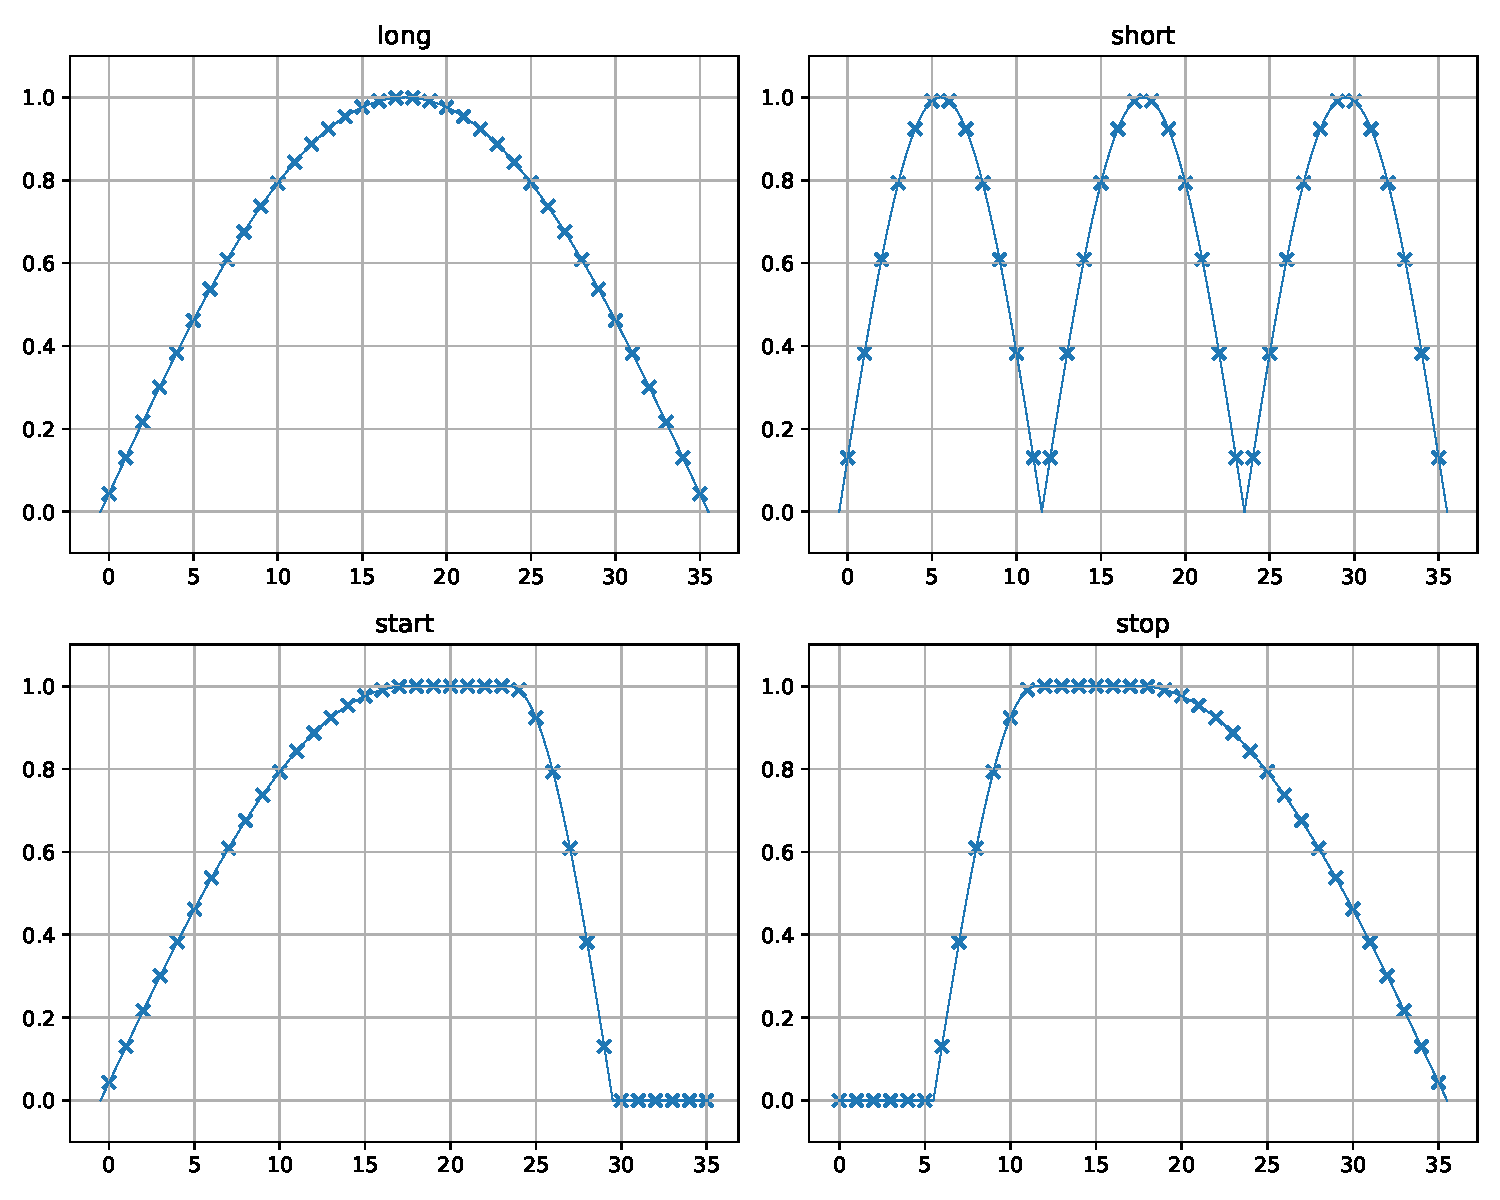
\includegraphics[width=105mm]{./figs/window_functions.pdf}
    \end{figure}
\end{frame}

\begin{frame}[c]
    \frametitle{MP3とMDCT -- 窓関数の状態遷移}
    \begin{figure}
        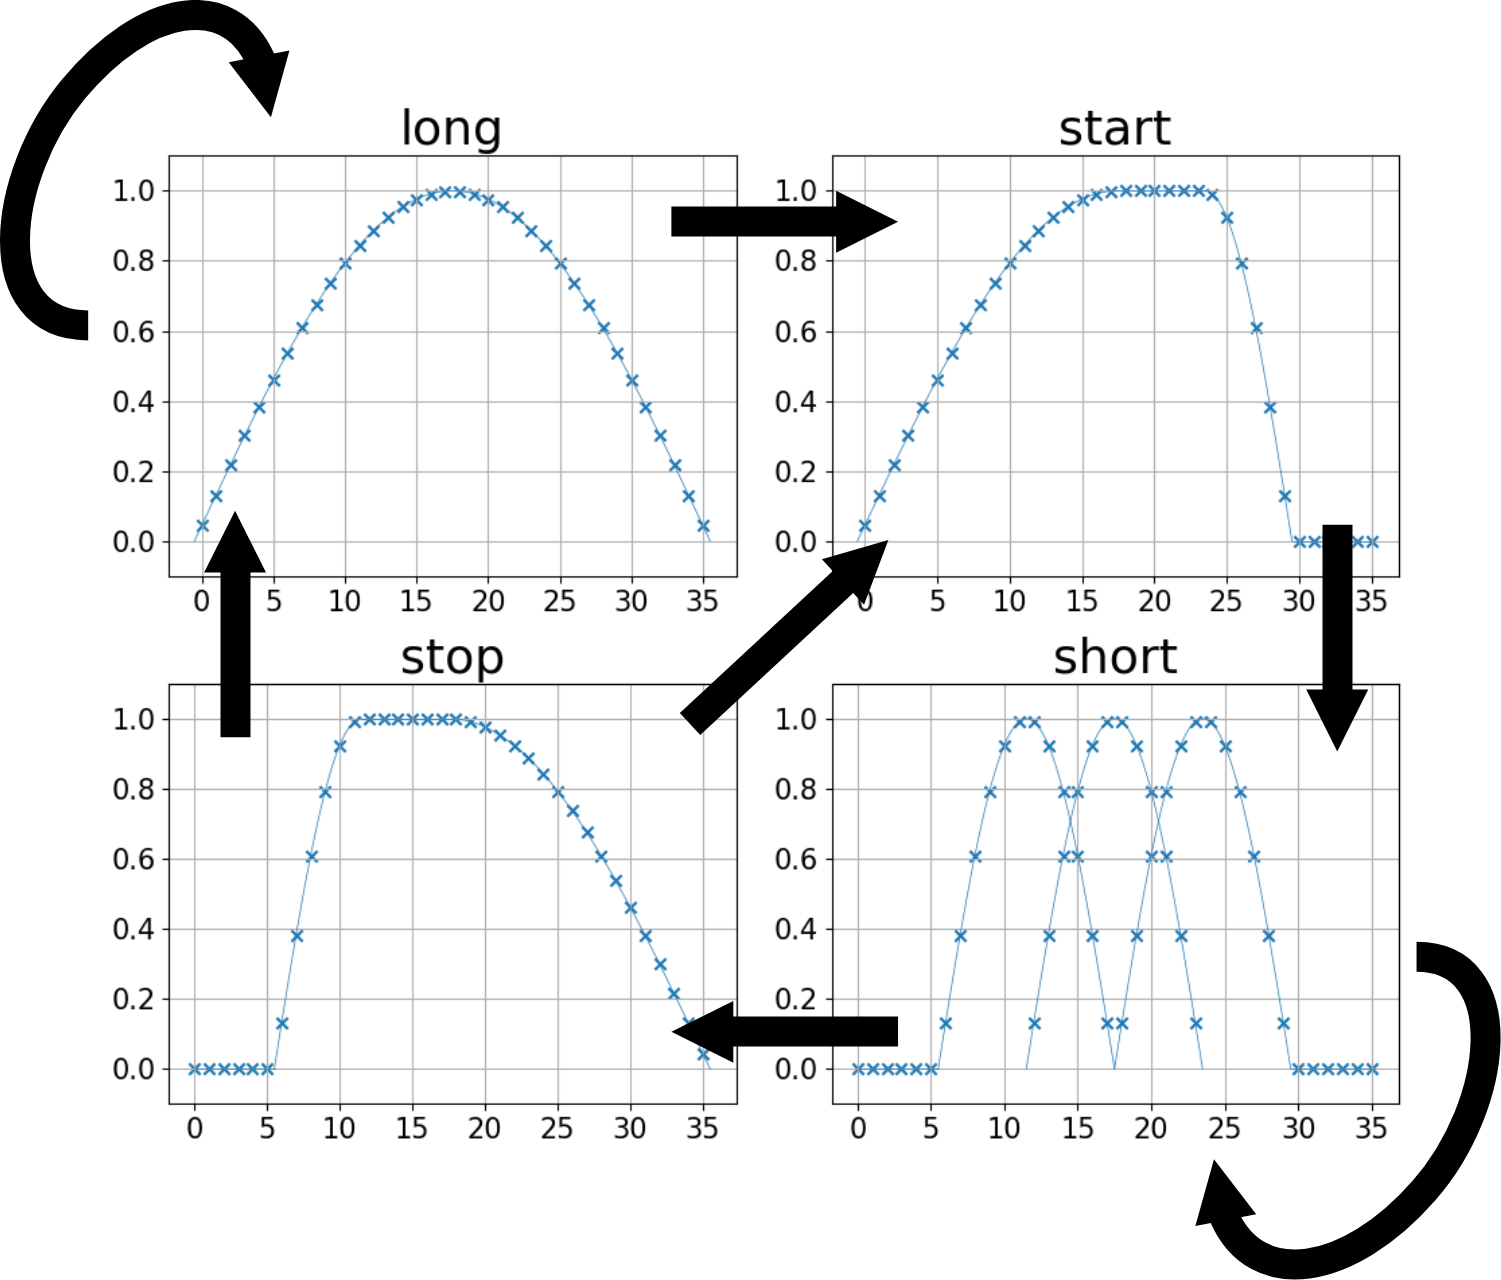
\includegraphics[width=98mm]{./figs/window_function_transition.png}
    \end{figure}
    \vspace{-27pt}
    状態遷移は聴覚心理モデルにより決定
\end{frame}

\begin{frame}[c]
    \frametitle{MP3とPrincen--Bradley条件}
    \begin{block}{}
        サイン窓
        \begin{align}
            w[n] = \sin \left[ \frac{\pi}{2N} \left( n + \frac{1}{2} \right) \right] \quad (n = 0, ..., 2N - 1)
        \end{align}
        はPrincen--Bradley条件を満たす.
    \end{block}
    \scriptsize
    (証明)式\eqref{eq:another_princen_bradley_conditon_1}は:
    \begin{align*}
        &w[n]^{2} + w[n + N]^{2} = \sin^{2} \left[ \frac{\pi}{2N} \left( n + \frac{1}{2} \right) \right] + \sin^{2} \left[ \frac{\pi}{2N} \left( n + N + \frac{1}{2} \right) \right] \\
        % &= \sin^{2} \left[ \frac{\pi}{2N} \left( n + \frac{1}{2} \right) \right] + \sin^{2} \left[ \frac{\pi}{2N} \left( n + \frac{1}{2} \right) + \frac{\pi}{2} \right] \\
        &= \sin^{2} \left[ \frac{\pi}{2N} \left( n + \frac{1}{2} \right) \right] + \cos^{2} \left[ \frac{\pi}{2N} \left( n + \frac{1}{2} \right) \right] = 1
    \end{align*}
    式\eqref{eq:another_princen_bradley_conditon_2}は,サイン窓が対称であることより示される:
    \begin{align*}
        & w[2N - 1 - n] = \sin\left[ \frac{\pi}{2N} \left( 2N - 1 - n + \frac{1}{2} \right) \right] = \sin\left[ \pi + \frac{\pi}{2N} \left( - n - \frac{1}{2} \right) \right] \\
        &= \sin \left[ -\frac{\pi}{2N} \left( n + \frac{1}{2} \right) + \pi \right] = \sin \left[ \frac{\pi}{2N} \left( n + \frac{1}{2} \right) \right] = w[n]
    \end{align*}
\end{frame}

\begin{frame}[c]
    \frametitle{MP3とPrincen--Bradley条件}
    \begin{itemize}
        \item long, short窓はサイン窓そのものなので完全再構成
        \item 状態遷移時に完全再構成になるか?
            \begin{enumerate}
                \item long $\rightarrow$ start
                \item stop $\rightarrow$ long:1.の対称ケース
                \item start $\rightarrow$ short
                \item short $\rightarrow$ stop:3.の対称ケース
            \end{enumerate}
            1.と3.だけ確認
    \end{itemize}
\end{frame}

\begin{frame}[c]
    \frametitle{MP3とPrincen--Bradley条件}
    \begin{columns}
        \begin{column}{0.45\textwidth}
            1. long $\rightarrow$ start
            \begin{itemize}
                \item ハーフオーバーラップアドする区間でサイン窓になっているため,完全再構成
            \end{itemize}
        \end{column}
        \begin{column}{0.55\textwidth}
            \begin{figure}
                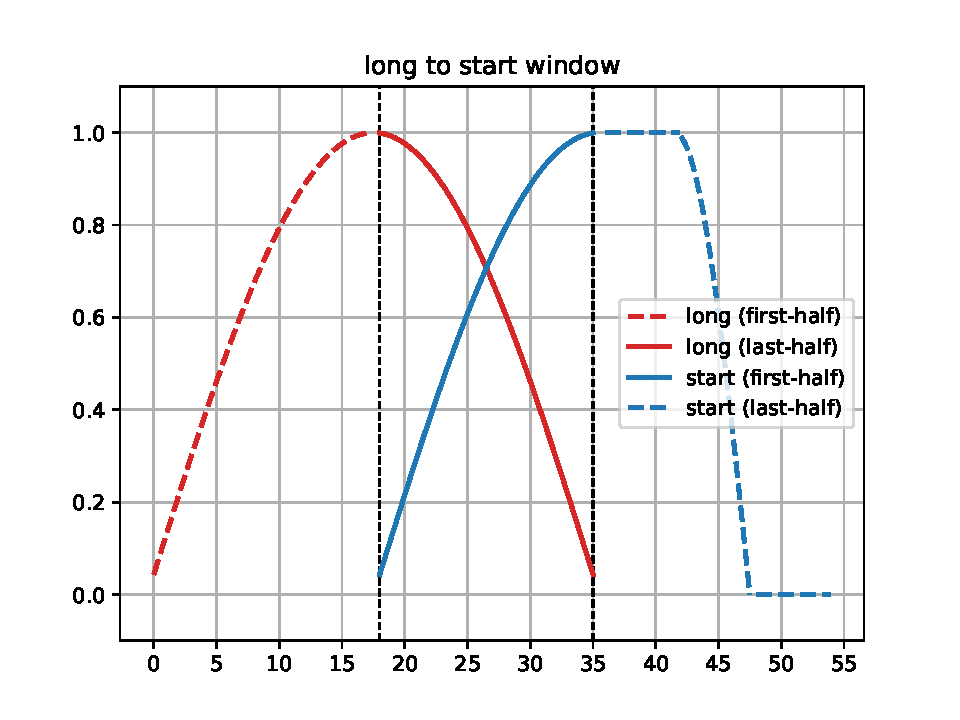
\includegraphics[width=68mm]{./figs/long_to_start_window.pdf}
            \end{figure}
        \end{column}
    \end{columns}
\end{frame}

\begin{frame}[c]
    \frametitle{MP3とPrincen--Bradley条件}
    \begin{columns}
        \begin{column}{0.45\textwidth}
            3. start $\rightarrow$ short
            \begin{itemize}
                \item $n = 0,...,5$:start窓が1, short窓が0なので完全再構成
                \item $n = 6,...,11$:サイン窓になっているため完全再構成
                \item $n = 12,...,17$:start窓が0, short窓どうしでサイン窓になっているため完全再構成
            \end{itemize}
        \end{column}
        \begin{column}{0.55\textwidth}
            \begin{figure}
                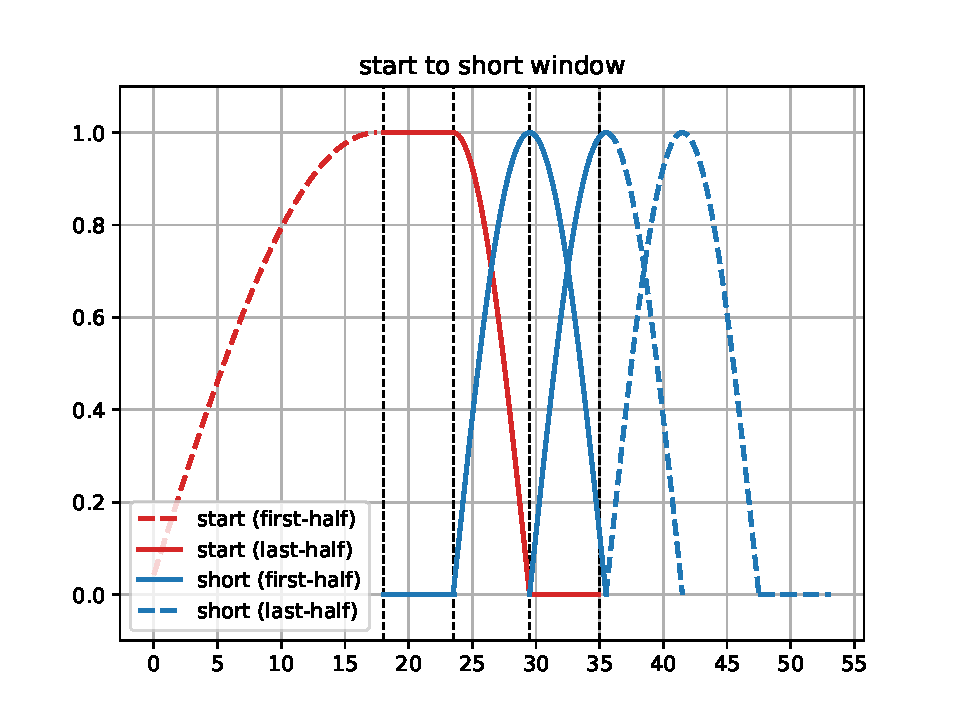
\includegraphics[width=68mm]{./figs/start_to_short_window.pdf}
            \end{figure}
        \end{column}
    \end{columns}
\end{frame}

\subsection{エイリアス削減バタフライ演算}

\begin{frame}[c]
    \frametitle{エイリアス削減バタフライ演算}
    \begin{columns}
        \begin{column}{0.35\textwidth}
            \begin{itemize}
                \item フィルタバンクは,隣接バンクの周波数成分(エイリアス)が混入
                \item 隣接バンクのスペクトルを使いエイリアス削減(\cite{edler1992aliasing})
            \end{itemize}
        \end{column}
        \begin{column}{0.7\textwidth}
            \begin{figure}
                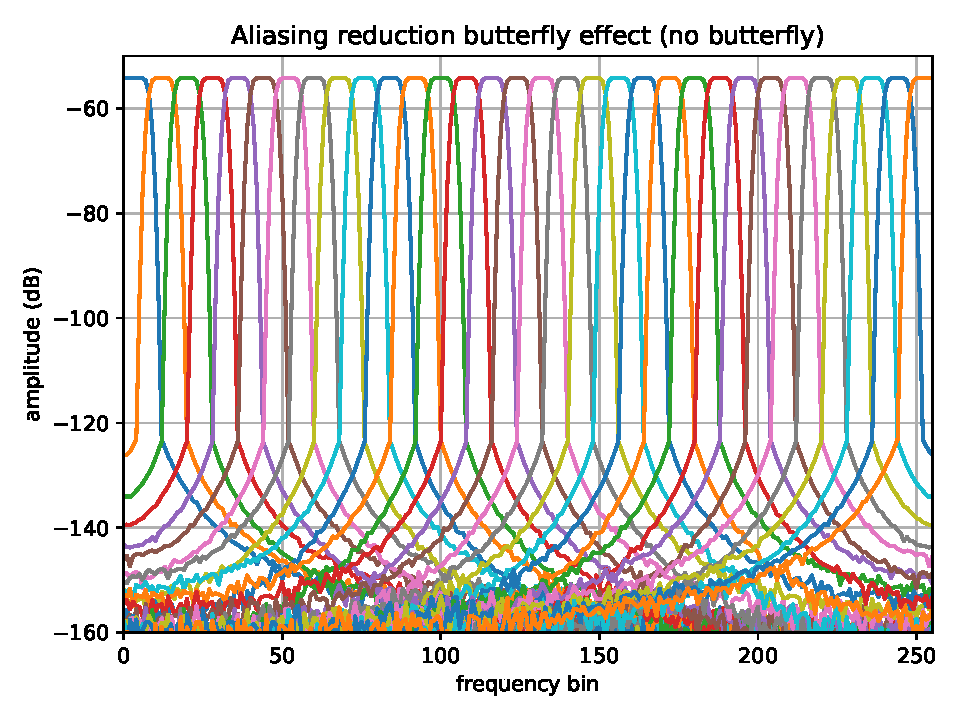
\includegraphics[width=85mm]{./figs/MP3_aliasing_reduction_butterfly_no_butterfly.pdf}
            \end{figure}
        \end{column}
    \end{columns}
\end{frame}

\begin{frame}[c]
    \frametitle{エイリアス削減バタフライ演算}
    \begin{columns}
        \begin{column}{0.55\textwidth}
            \small
            \begin{itemize}
                \item スペクトルを$X_{k}$としたとき,
                    \begin{align}
                        X_{18k - i} &\leftarrow \mathrm{cs}_{i} X_{18k - i} - \mathrm{ca}_{i} X_{18k + i + 1} \\
                        X_{18k + i + 1} &\leftarrow \mathrm{ca}_{i} X_{18k - i} + \mathrm{cs}_{i} X_{18k + i + 1} \\
                        & k = 1,...,31,\ i = 0,...,7 \nonumber
                    \end{align}
                \item 係数$\mathrm{cs}_{i},\mathrm{ca}_{i}$の定義
                    \begin{align}
                        \mathrm{cs}_{i} := \frac{1}{\sqrt{1 + c_{i}^{2}}},\ \mathrm{ca}_{i} := \frac{c_{i}}{\sqrt{1 + c_{i}^{2}}}
                    \end{align}
                    $c_{i}\ (i=0,...7)$は規格で設定
            \end{itemize}
        \end{column}
        \begin{column}{0.45\textwidth}
            \begin{figure}
                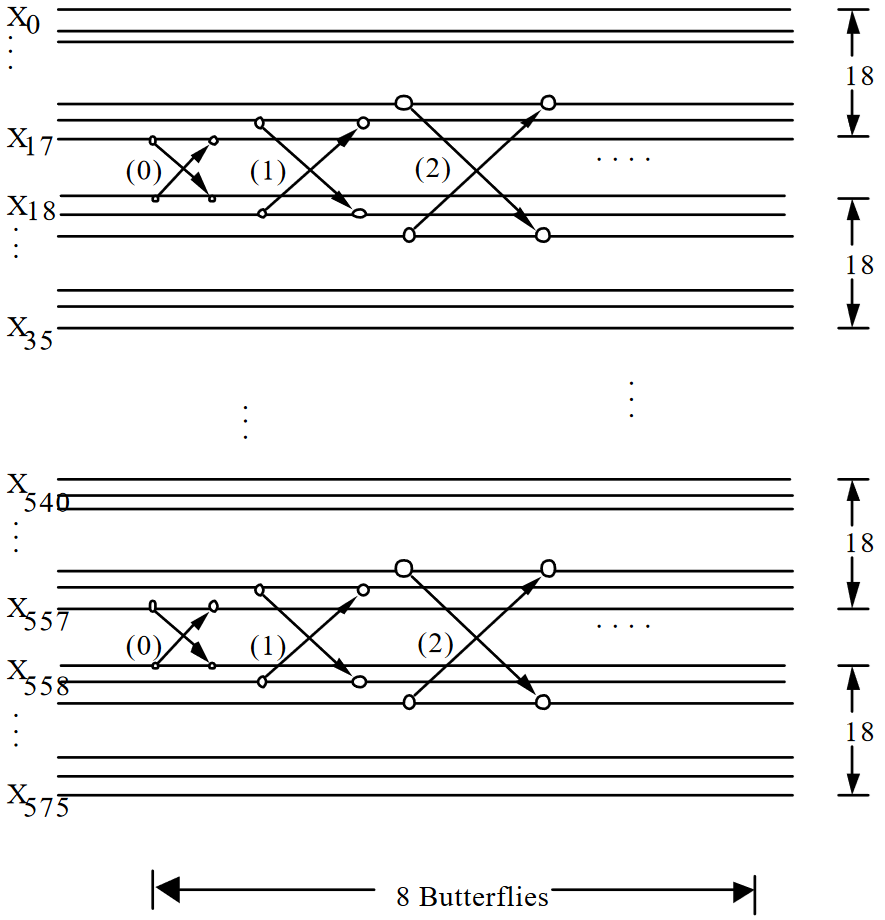
\includegraphics[width=52mm]{./figs/butterfly_reduction_alias.png}
                \caption*{\cite{raissi2002theory}より引用}
            \end{figure}
        \end{column}
        \end{columns}
\end{frame}

\begin{frame}[c]
    \frametitle{エイリアス削減バタフライ演算}
    \begin{columns}
        \begin{column}{0.35\textwidth}
            \begin{itemize}
                \item 14-17バンドの周波数特性比較
                \item バタフライ演算により,隣接バンクと交差する振幅が-2dBほど下に移動(改善)
            \end{itemize}
        \end{column}
        \begin{column}{0.7\textwidth}
            \begin{figure}
                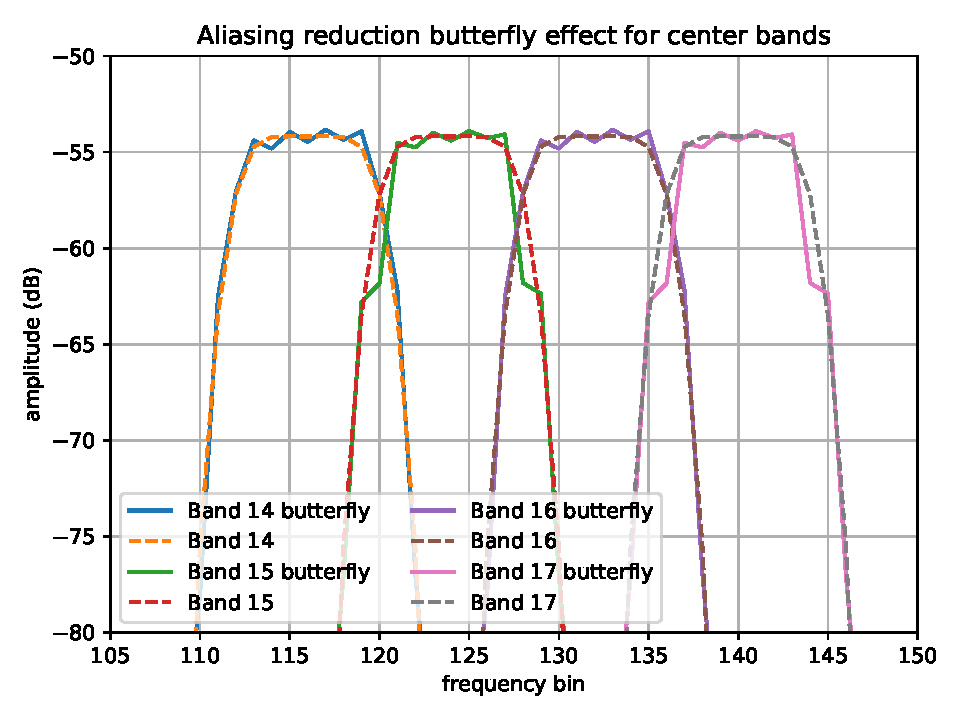
\includegraphics[width=85mm]{./figs/MP3_aliasing_reduction_butterfly_focusbands.pdf}
            \end{figure}
        \end{column}
    \end{columns}
\end{frame}

\begin{frame}[c]
    \frametitle{エイリアス削減バタフライ演算}
    \begin{columns}
        \begin{column}{0.35\textwidth}
            \begin{itemize}
                \item 振幅が小さくなると遮断特性は悪化
                \item 可聴域帯を優先した結果?
            \end{itemize}
        \end{column}
        \begin{column}{0.7\textwidth}
            \begin{figure}
                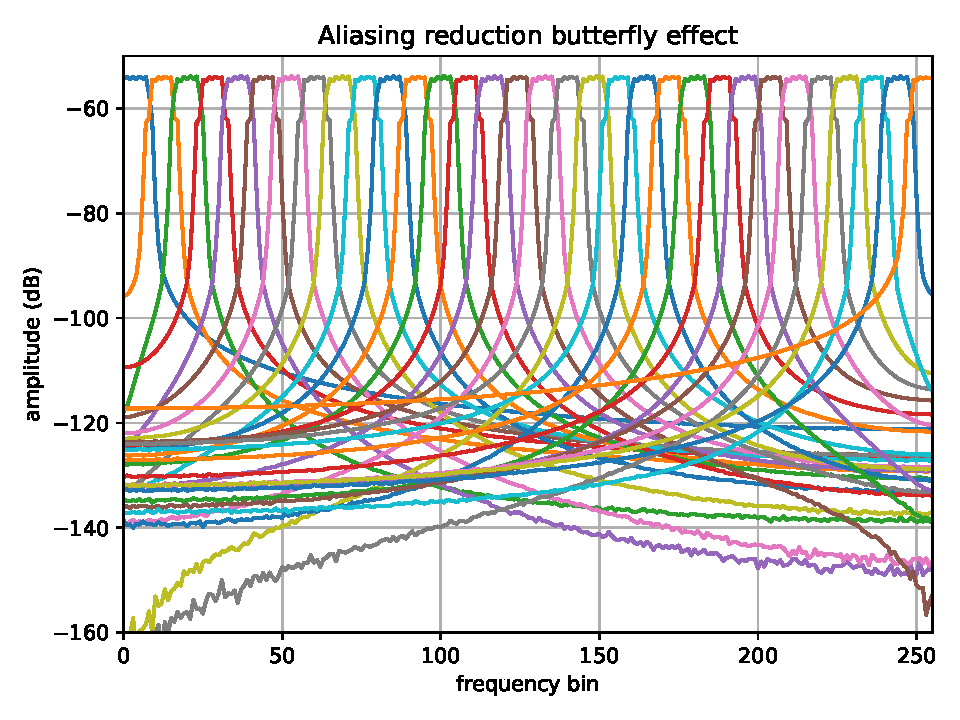
\includegraphics[width=85mm]{./figs/MP3_aliasing_reduction_butterfly_butterfly.pdf}
            \end{figure}
        \end{column}
    \end{columns}
\end{frame}

\section{量子化}

\begin{frame}[c]
    \frametitle{非線形量子化}
    ブロック長が36(long, start, stop)のとき,量子化スペクトル$X_{i}^{q}$,逆量子化スペクトル$\hat{X}_{i}$は
    \footnote{
        $\mathrm{round}$を除けば,逆量子により元に戻る
        \vspace{-5pt}
        \begin{align*}
            \hat{X}_{i} = \mathrm{sign}(X_{i}) |X_{i}^{q}|^{\frac{4}{3}} G^{l}_{i} = \mathrm{sign}(X_{i}) \left| | X_{i} (G_{i}^{l})^{-1} |^{\frac{3}{4}} \right|^{\frac{4}{3}} G_{i}^{l} = X_{i} (G_{i}^{l})^{-1} G_{i}^{l} = X_{i}
        \end{align*}}
    \begin{align}
        X_{i}^{q} &= \mathrm{round}\left[ \mathrm{sign}(X_{i}) \left| X_{i} (G^{l}_{i})^{-1} \right|^{\frac{3}{4}} \right] \\
        \hat{X}_{i} &= \mathrm{sign}(X_{i}^{q}) |X_{i}^{q}|^{\frac{4}{3}} G^{l}_{i} \\
        G^{l}_{i} &= 2^{\frac{1}{4}g} 2^{-\frac{1}{2} (1 + \mathrm{scale})(\mathrm{sl}_{i} + p_{i})}
    \end{align}
    \vspace{-20pt}
    \small
    \begin{itemize}
        \item $g$:グローバルゲイン
        \item $\mathrm{scale}$:スケールファクタのスケール{\scriptsize(dist10エンコーダーでは常に0)}
        \item $\mathrm{sl}_{i}$:スケールファクタ
        \item $p_{i}$:プリエンファシス増幅値{\scriptsize(dist10エンコーダーでは常に0)}
    \end{itemize}
\end{frame}

\begin{frame}[c]
    \frametitle{非線形量子化}
    ブロック長が12(short)のとき,
    \begin{align}
        X_{i}^{q} &= \mathrm{round}\left[ \mathrm{sign}(X_{i}) \left| X_{i} (G_{i}^{s})^{-1} \right|^{\frac{3}{4}} \right] \\
        \hat{X}_{i} &= \mathrm{sign}(X_{i}^{q}) |X_{i}^{q}|^{\frac{4}{3}} G_{i}^{s} \\
        G^{s}_{i} &= 2^{\frac{1}{4}g} 2^{2\mathrm{sbgain}_{b}} 2^{-\frac{1}{2} (1 + \mathrm{scale})\mathrm{ss}_{i}}
    \end{align}
    \vspace{-20pt}
    \small
    \begin{itemize}
        \item $\mathrm{sbgain}_{b}$:サブブロックのゲイン{\scriptsize(dist10エンコーダーでは常に0)}
        \item $\mathrm{ss}_{i}$:ショートブロックのスケールファクタ
    \end{itemize}
\end{frame}

% \begin{frame}[c]
%     \frametitle{$3/4$乗の効果}
%     平均0分散0.1のLaplace分布の絶対値$|x|$と$|x|^{\frac{3}{4}}$の密度
%     \begin{figure}
%         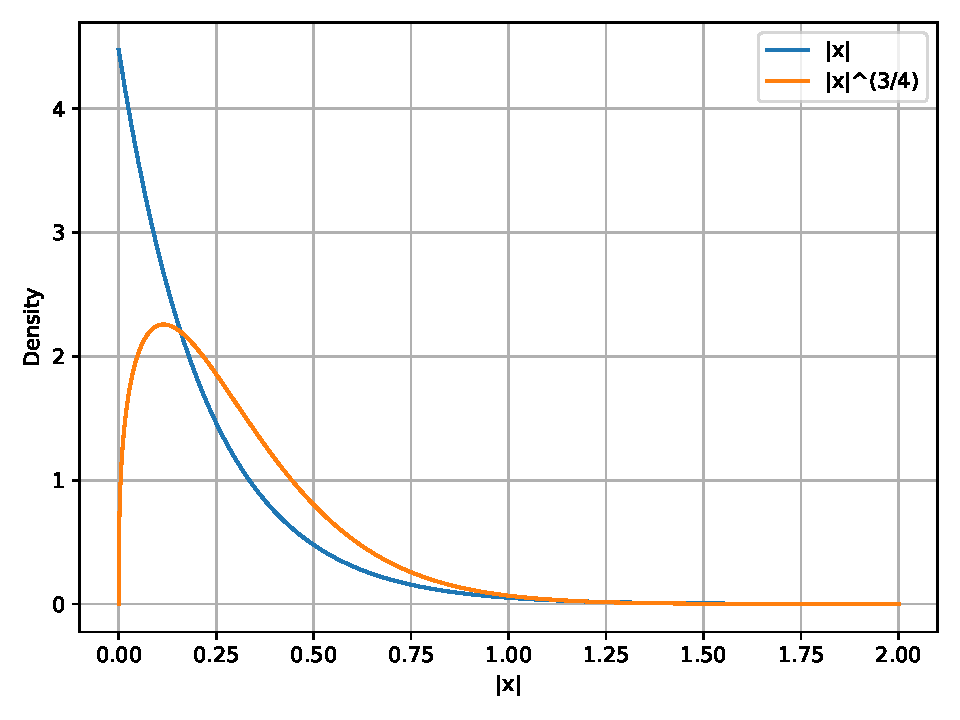
\includegraphics[width=90mm]{./figs/powered_distribution.pdf}
%     \end{figure}
%     \vspace{-10pt}
%     $0$近傍の密度が減少
% \end{frame}

\begin{frame}[c]
    \frametitle{$3/4$乗の効果}
    $x, x^{\frac{3}{4}}$とそれらの微分(ステップ幅)
    \begin{figure}
        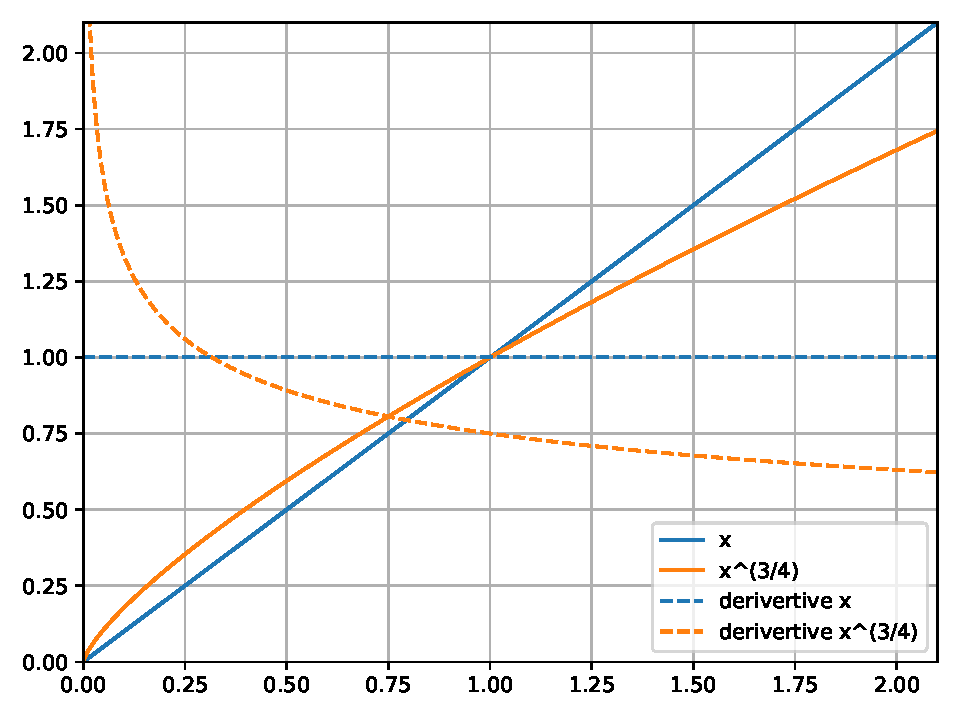
\includegraphics[width=90mm]{./figs/powered_quantization_curve.pdf}
    \end{figure}
    \vspace{-10pt}
    $0$近傍は荒く量子化,$\approx 0.3$以上では細かく量子化
\end{frame}

\section{符号化}

\begin{frame}[c]
    \frametitle{MP3の符号化}
    量子化スペクトルを区分に分けて符号化
    \begin{figure}
        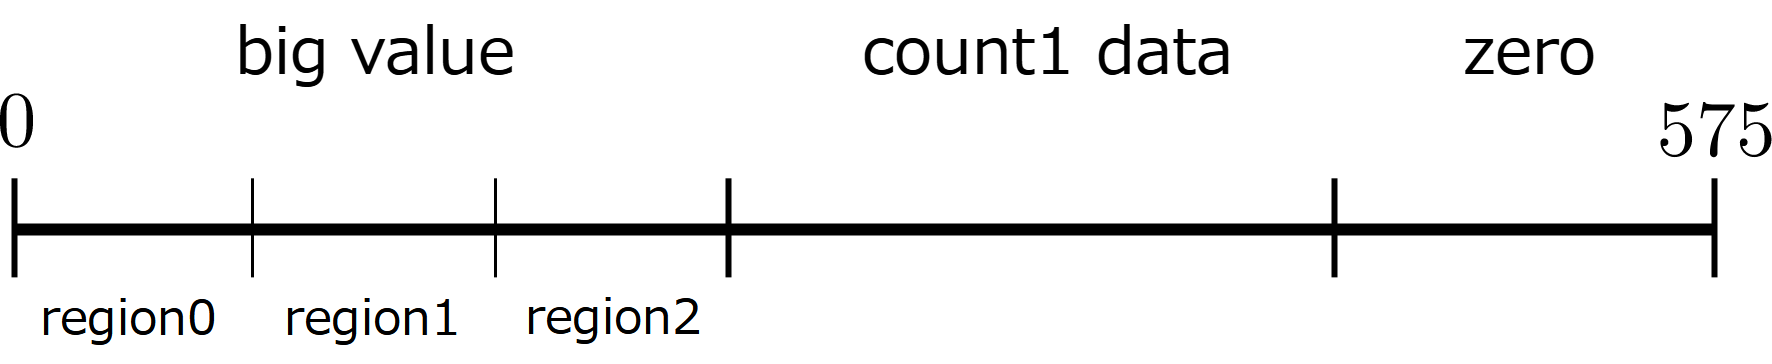
\includegraphics[width=115mm]{./figs/huffman_coding_region_division.png}
    \end{figure}
    \begin{description}
        \item[big value] 大きい値は線形量子化を兼用
            \begin{itemize}
                \item region0,1,2で異なるハフマンテーブルを使用
            \end{itemize}
        \item[count1 data] $\{ -1, 0, 1 \}$のみで符号化
            \begin{itemize}
                \item 1つのハフマンテーブルを使用
            \end{itemize}
        \item[zero] $0$のみ(符号化しない)
    \end{description}
    % MDCTは低域に成分集中するため,妥当な符号化
\end{frame}

\begin{frame}[c]
    \frametitle{MP3の符号化(詳細)}
    \structure{big valueの符号化}
    \begin{itemize}
        \item 数値2つ組$X_{i}^{q}, X_{i+1}^{q}$を
            \begin{align}
                X = 16 |X_{i}^{q}| + |X_{i+1}^{q}|
            \end{align}
            として符号化.符号は2bitで出力
        \item 線形符号化するかの閾値はテーブル毎に設定
    \end{itemize}
    \structure{count1 dataの符号化}
    \begin{itemize}
        \item 数値4つ組$X_{i}^{q}, X_{i+1}^{q}, X_{i+2}^{q}, X_{i+3}^{q}$を
            \begin{align}
                X = 8 s(X_{i+2}^{q}) + 4 s(X_{i+3}^{q}) + 2 s(X_{i}^{q}) + s(X_{i+1}^{q})
            \end{align}
            として符号化($s(x)$:$x\neq 0$なら$1$,$x=0$なら$0$).符号は4bitで出力
    \end{itemize}
\end{frame}

\section{聴覚心理モデルII}

\begin{frame}[c]
    \frametitle{聴覚心理モデルIIの概要}
    \begin{itemize}
        \item LayerIIIの聴覚心理モデル(LayerI, IIとは異なる)
        \item 出力:信号対マスク比(SMR\footnote{Signal-to-Masking Ratio}),ブロックタイプ
        \item 処理手順
            \begin{enumerate}
                \item フレーム切り出し・窓かけ・FFT
                \item Unpredictability計算
                \item パーティションごとのエネルギー計算
                \item 広がり関数(Spreading function)の畳み込み
                \item ノイズ許容レベル計算
                \item 聴覚しきい値計算
                \item 知覚エントロピー(Psychoacoustic entropy)計算・ブロックタイプ判定
                \item 信号対マスク比(SMR)計算
            \end{enumerate}
    \end{itemize}
\end{frame}

\begin{frame}[c]
    \frametitle{フレーム切り出し・窓かけ・FFT}
    \begin{itemize}
        \item longとshortの2つを計算
            \begin{itemize}
                \item longはサイズ1024
                \item shortはサイズ256を3つ.信号$s[n]$の$s[128b + n]\ b = 1,2,3$を使用
            \end{itemize}
        \item Hanning窓を適用
        \item スライド(hop)サイズは576($=$DCTスペクトルサイズ)
    \end{itemize}
    FFT係数を$w^{l}$(long),$w^{s_{b}}$(short, $b=1,2,3$)と表記
\end{frame}

\begin{frame}[c]
    \frametitle{フレーム切り出し・窓かけ・FFT}
    \begin{figure}
        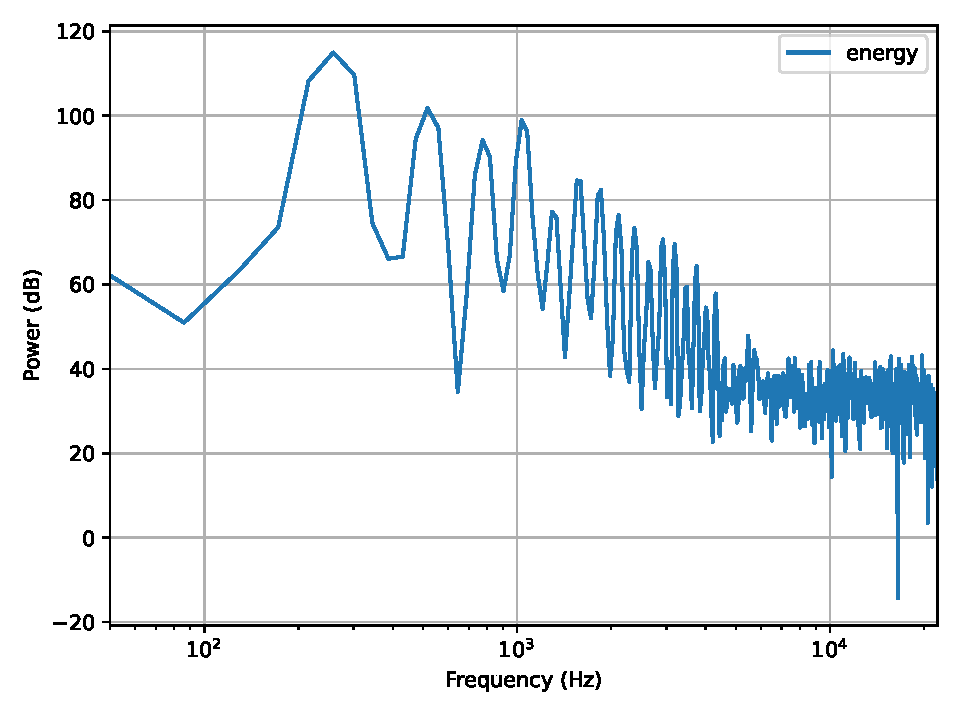
\includegraphics[width=100mm]{./figs/psyco_analyze_energy.pdf}
        \caption*{ピアノ($F_{0}$=220)のlongのエネルギー(パワースペクトル)}
    \end{figure}
\end{frame}

\begin{frame}[c]
    \frametitle{Unpredictability計算}
    Unpredictability $cw$ = 予測しずらさの尺度
    \small
    \begin{align}
        cw[n] = \left\{ \begin{array}{cl}
            \frac{|w^{l}[n] - w^{l\ast}[n]|}{|w^{l}[n]| + |w^{l\ast}[n]|} & 0 \leq n \leq 5 \\
            \frac{|w^{s_{2}}[j] - w^{s\ast}[j]|}{|w^{s_{2}}[j]| + |w^{s\ast}[j]|} & j = \lfloor (n + 2)/4 \rfloor,\ 6 \leq n \leq 205 \\
            0.4 & 206 \leq n \leq 512
        \end{array} \right.
    \end{align}
    \normalsize
    \begin{itemize}
        \item $w^{l\ast}, w^{s\ast}$:振幅と位相を直線予測したスペクトル
            \begin{itemize}
                \item 直線予測の式($w^{l\prime}$は前フレームの$w^{l}$):
                    \footnotesize
                    \begin{align}
                        w^{l\ast}[n] &= (2|w^{l\prime}[n]| - |w^{l\prime\prime}[n]|) \exp[j (2\arg(w^{l\prime}[n]) - \arg(w^{l\prime\prime}[n]))] \\
                        w^{s\ast}[n] &= (2|w^{s_{1}}[n]| - |w^{s_{3}}[n]|) \exp[j (2\arg(w^{s_{1}}[n]) - \arg(w^{s_{3}}[n]))]
                    \end{align}
            \end{itemize}
        \item 予測が当たれば$cw[n] = 0$,外れると$cw[n] = 1$
    \end{itemize}
\end{frame}

\begin{frame}[c]
    \frametitle{パーティションごとのエネルギー計算}
    周波数ビンを"パーティション(partition)"単位に分割
    \begin{itemize}
        \item $eb^{l}, eb^{s}$:パーティション内のエネルギーを合算
        \item $cb$:Unpredictabilityで重みづけしたエネルギーを合算
    \end{itemize}
    long, shortのパーティション$b$を$P^{l}_{b}, P^{s}_{b}$と書くと,
    \small
    \begin{align}
        eb^{l}[b] &= \sum_{n = \min P^{l}_{b}}^{\max P^{l}_{b} - 1} |w^{l}[n]|^{2} \\
        cb[b] &= \sum_{n = \min P^{l}_{b}}^{\max P^{l}_{b} - 1} cw[n] |w^{l}[n]|^{2} \\
        eb^{s}[b] &= \sum_{n = \min P^{s}_{b}}^{\max P^{s}_{b} - 1} |w^{s}[n]|^{2}
    \end{align}
\end{frame}

\begin{frame}[c]
    \frametitle{パーティションごとのエネルギー計算}
    \begin{figure}
        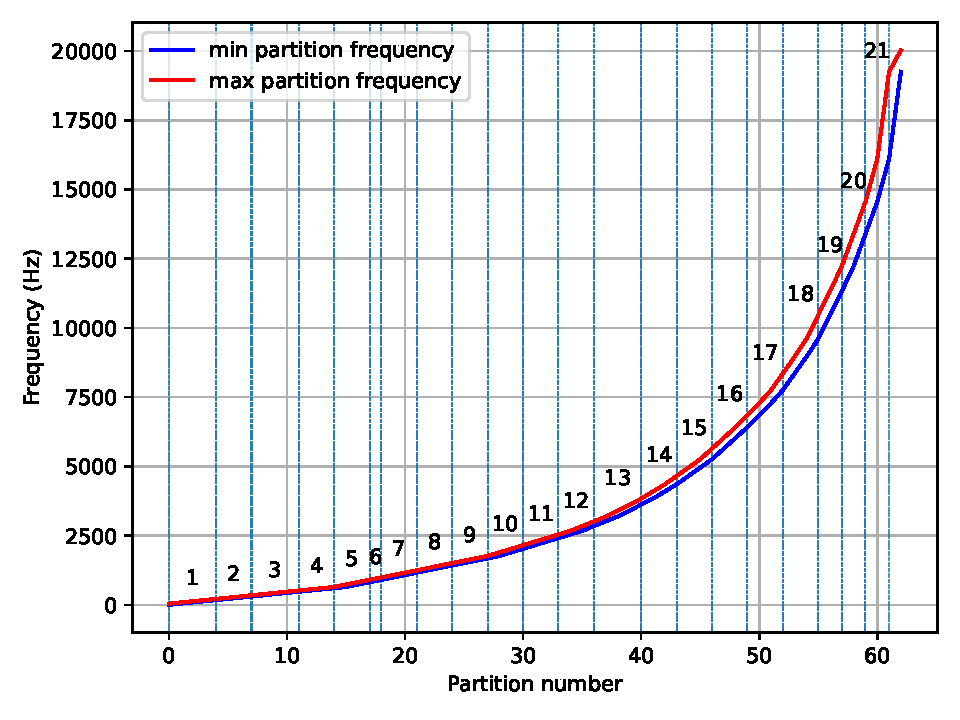
\includegraphics[width=95mm]{./figs/partion_frequency_long44100Hz.pdf}
        \caption*{サンプリング周波数44.1kHzのlongのパーティション.Barkスケールを細かくしたものとみなせる}
    \end{figure}
\end{frame}

\begin{frame}[c]
    \frametitle{パーティションごとのエネルギー計算}
    \begin{figure}
        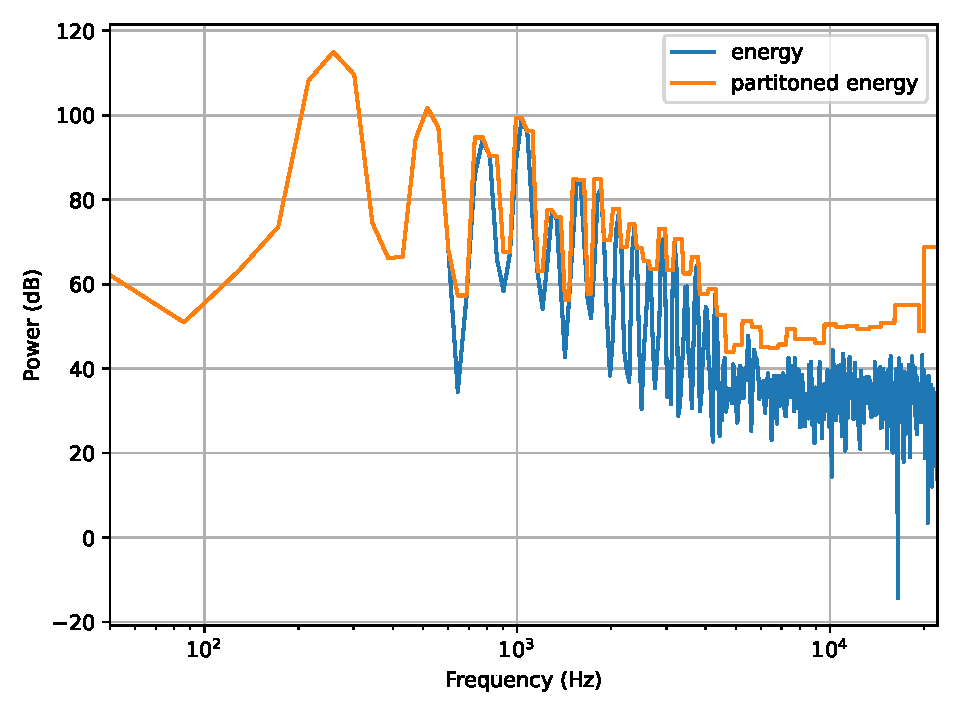
\includegraphics[width=100mm]{./figs/psyco_analyze_partitioned_energy.pdf}
        \caption*{ピアノ($F_{0}$=220)のlongパーティション分割後のエネルギー$eb^{l}$}
    \end{figure}
\end{frame}

\begin{frame}[c]
    \frametitle{広がり関数の畳み込み}
    エネルギーに広がり関数(Spreading function)$SF^{l}_{b}, SF^{s}_{b}$を畳み込み,調波成分のマスキングを考慮
    \begin{itemize}
        \item $ecb^{l}, ecb^{s}$:$SF^{l}_{b}, SF^{s}_{b}$を畳みこんだ$eb^{l}, eb^{s}$
        \item $ctb$:$SF^{l}_{b}$を畳みこんだ$cb$
    \end{itemize}
    \begin{align}
        ecb^{l}[b] &= \sum_{k} SF^{l}_{b}[k] eb^{l}[k] \\
        ctb[b] &= \sum_{k} SF^{l}_{b}[k] cb[k] \\
        ecb^{s}[b] &= \sum_{k} SF^{s}_{b}[k] eb^{s}[k]
    \end{align}
\end{frame}

\begin{frame}[c]
    \frametitle{広がり関数の概形}
    \begin{figure}
        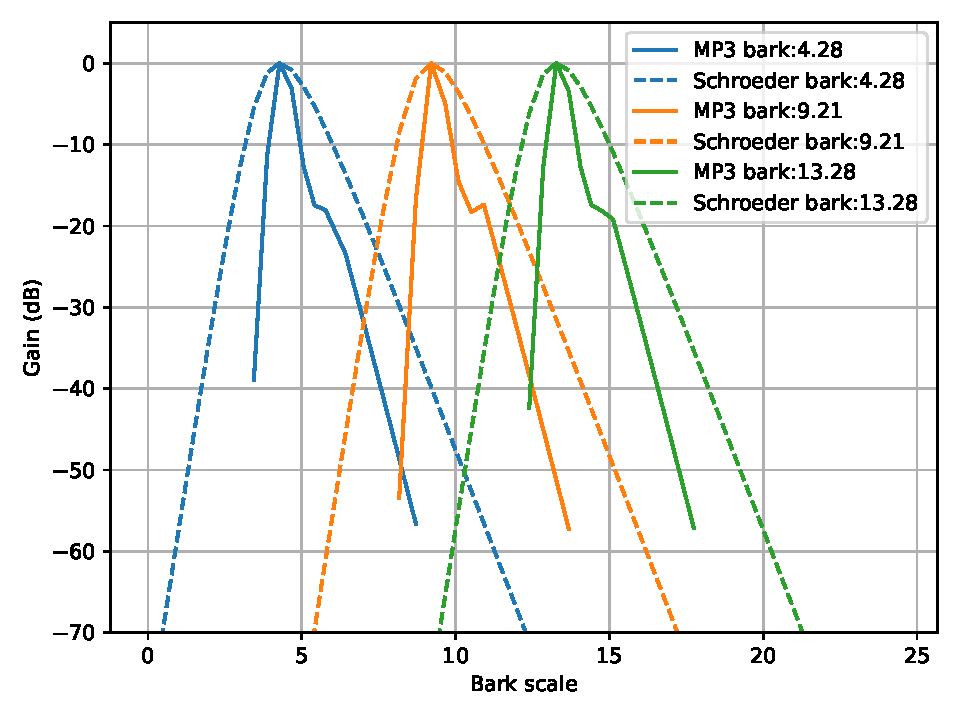
\includegraphics[width=95mm]{./figs/spreading_functons.pdf}
        \caption*{いくつかのバーク値での広がり関数.MP3では-60dB以下のスケールは0に丸め込むため線が途切れている.}
    \end{figure}
\end{frame}

\begin{frame}[c]
    \frametitle{広がり関数の畳み込み}
    \begin{figure}
        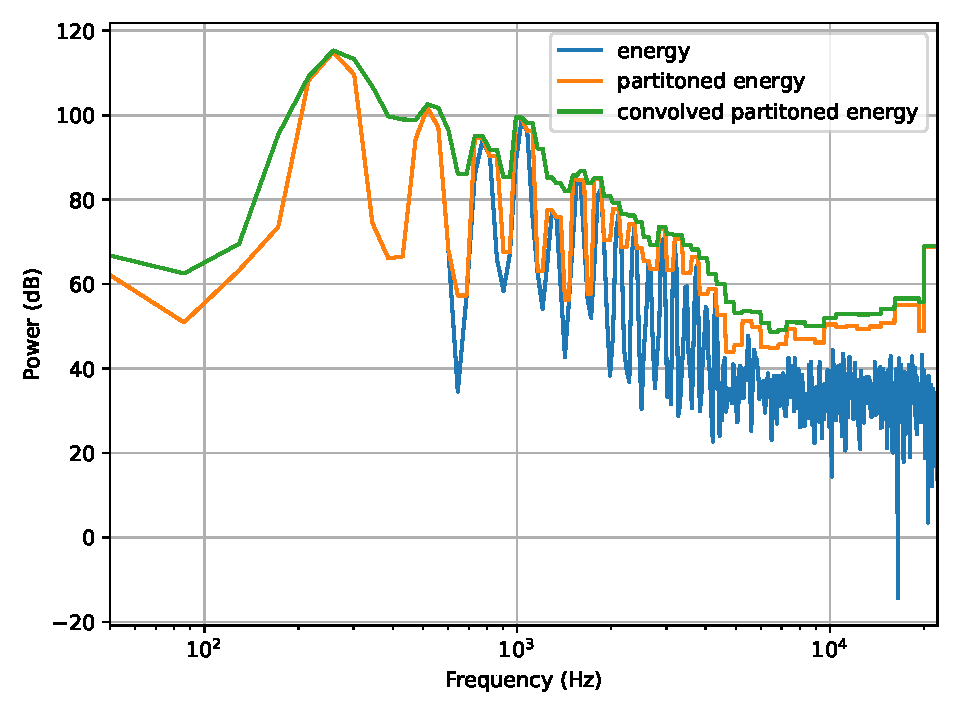
\includegraphics[width=100mm]{./figs/psyco_analyze_convolved_partitioned_energy.pdf}
        \caption*{ピアノ($F_{0}$=220)の広がり関数を畳みこんだエネルギー$ecb^{l}$}
    \end{figure}
\end{frame}

\begin{frame}[c]
    \frametitle{ノイズ許容レベル計算}
    パーティション$b$の量子化ノイズ許容レベルを計算\footnote{shortは省略.SNRをテーブル引きして計算する以外同様のため}
    \small
    \begin{description}
        \item[$tbb$計算] $tbb=0$はノイズ,$tbb=1$は調波成分を示す尺度
            \begin{align}
                cbb &= \log \left( \max \left\{ \frac{ctb[b]}{ecb^{l}[b]}, 0.01 \right\} \right) \\
                tbb &= \min\{ 1.0, \max\{ 0.0, - 0.299 - 0.43 cbb \} \}
            \end{align}
        \item[SNR計算] マスクの加重和でSNR(dB)を計算.$29.0$は調波によるノイズのマスク,$6.0$はノイズによる純音のマスク
            \begin{align}
                snr = \max \left\{ \mathrm{minval}_{b}, 29.0 tbb + 6.0 (1 - tbb) \right\}
            \end{align}
        \item[許容レベル計算] SNRにエネルギーを乗じて許容レベル$nb^{l}$を得る.広がり関数で増えたエネルギーを戻す
            \begin{align}
                nb^{l}[b] = \frac{ecb^{l}[b]}{\sum_{k} SF_{b}[k]} \times 10^{-\frac{snr}{10}}
            \end{align}
    \end{description}
\end{frame}

\begin{frame}[c]
    \frametitle{ノイズ許容レベル計算}
    \begin{figure}
        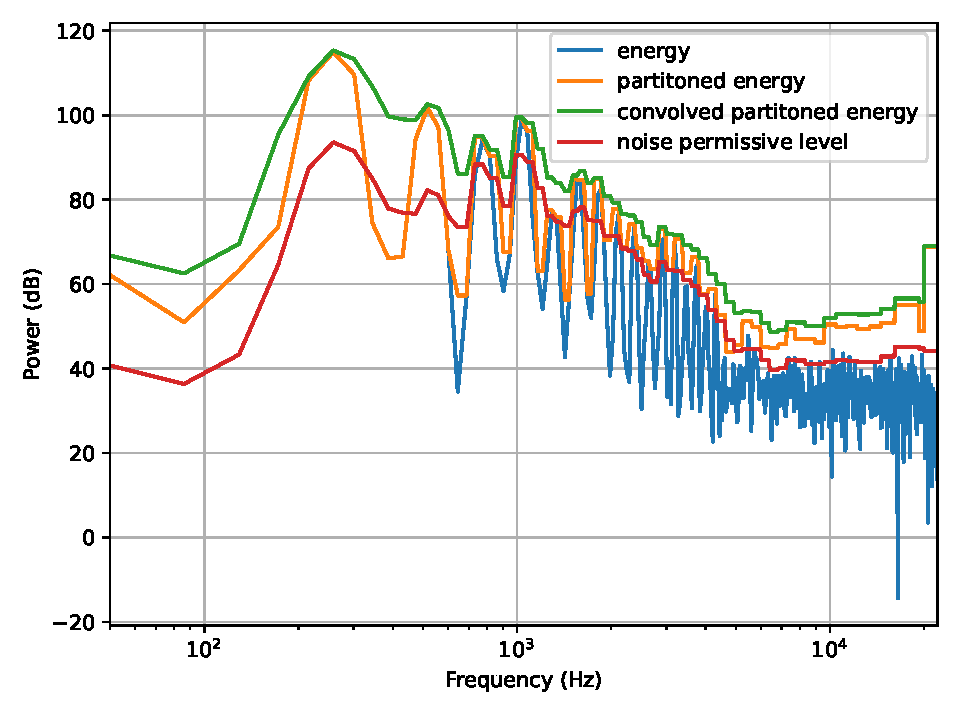
\includegraphics[width=100mm]{./figs/psyco_analyze_noise_permissive_level.pdf}
        \caption*{ピアノ($F_{0}$=220)のノイズ許容レベル$nb^{l}$}
    \end{figure}
\end{frame}

\begin{frame}[c]
    \frametitle{聴覚しきい値計算}
    前フレームのノイズ許容レベルと最小可聴パワーを考慮し,これを聴覚しきい値$thr^{l}$とする
    \begin{align}
        thr^{l}[b] = \max \left\{ \mathrm{qthr}_{b}, \min \{ 2nb^{l\prime}[b], 16nb^{l\prime\prime}[b], nb^{l}[b] \} \right\}
    \end{align}
    \begin{itemize}
        \item $\mathrm{qthr}_{b}$:最小可聴パワー
        \item $nb^{l\prime}, nb^{l\prime\prime}$:前とさらにその前のノイズ許容レベル
            \begin{itemize}
                \item 前フレームのノイズを残す.プリエコー対策
            \end{itemize}
    \end{itemize}
\end{frame}

\begin{frame}[c]
    \frametitle{聴覚しきい値計算}
    \begin{figure}
        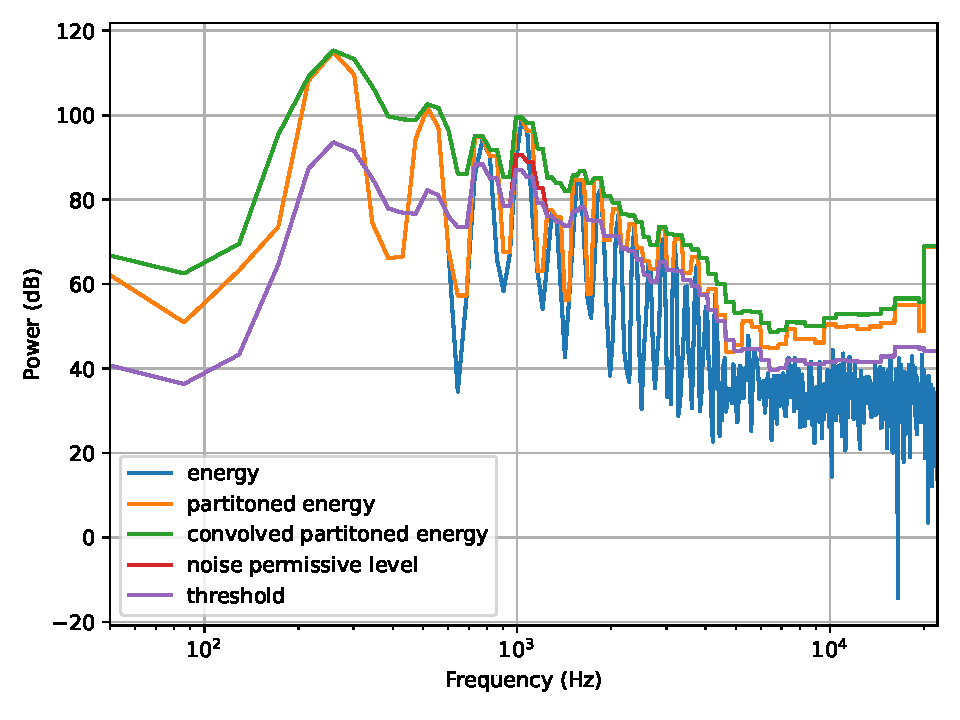
\includegraphics[width=100mm]{./figs/psyco_analyze_threshold.pdf}
        \caption*{ピアノ($F_{0}$=220)の聴覚しきい値$thr^{l}$}
    \end{figure}
\end{frame}

\begin{frame}[c]
    \frametitle{知覚エントロピー計算}
    知覚エントロピー$\mathrm{PE}$を以下で計算
    \begin{align}
        \mathrm{PE} = \sum_{b} |P^{l}_{b}| \log \frac{eb^{l}[b] + 1}{thr^{l}[b]}
    \end{align}
    フレームの符号化に必要なビット数の目安\footnote{導出は補足\ref{sec:proofs_perceptual_entropy}参照}
    \begin{itemize}
        \item $\mathrm{PE} \geq 1800$ならばshortブロックと判定.さもなくばlongブロックと判定\footnote{dist10では以前のブロック判定結果を保持している.判定とブロックの状態遷移に従い結果をstart,stopに変更}
    \end{itemize}
\end{frame}

% TODO: ピアノ音源で知覚エントロピーをプロット

\begin{frame}[c]
    \frametitle{信号対マスク比計算}
\end{frame}

\appendix

\section{参考文献}

\begin{frame}{参考文献の紹介}
    \scriptsize
    \begin{itemize}
        \item \cite{edler1992aliasing,liu1997design}:エイリアス削減の論文
        \item \cite{princen1986analysis}:Princen--Bradleyの完全再構成条件の導出
        \item \cite{raissi2002theory}:MP3の概要説明.
        \item \cite{fujiwara2001}:MPEG/Audioの他,2000年代前半の他のコーデックの概要を解説
        \item \cite{yasuda1994}:MPEG標準化に関する書物.技術は概要程度
        \item \cite{kiya1995}:マルチレートに関わる信号処理を広範に解説
        \item \cite{vaidyanathan2002}:フィルタバンクに関する詳細書
        \item \cite{kiya1997}:DCTに関する詳しい解説
        \item \cite{kosugi200108,kosugi200109,kosugi200111,kosugi200201,kosugi200202}:技術解説と簡易MP3コーデックの実装例
        \item \cite{urata1999}:MP3のソース(dist10)の解説.ただし木を見て森を見ずな印象.実装の補足説明としては優秀だが,コードを数式に直訳した書き方のため,理解しずらい.
        \item \cite{johnston1988estimation}:ノイズマスキングを用いた知覚エントロピーの考え方についての原論文
    \end{itemize}
\end{frame}

\begin{frame}[allowframebreaks]{参考文献}
    \printbibliography[heading=none]
\end{frame}

\section{証明}

\subsection{フィルタバンク} \label{sec:proofs_filter_bank}

\begin{frame}[c]
    \frametitle{完全再構成}
    遅延・定数倍を除き入出力が一致すること:
    \begin{align}
        \hat{x}[n] = c x[n - n_{0}], \quad c \neq 0
    \end{align}
    これは$z$領域で,
    \begin{align}
        \hat{X}(z) = c z^{-n_{0}} X(z)
    \end{align}
    となることと等価
\end{frame}

\begin{frame}[c]
    \frametitle{ポリフェーズ表現}
    $H_{k}(z)$のインパルス応答を$h_{k}[n]$と書くとき,
    \small
    \begin{align*}
        H_{k}(z) &= \sum_{n = -\infty}^{\infty} h_{k}[n] z^{-n} = \sum_{n = -\infty}^{\infty} \sum_{l = 0}^{M - 1} h_{k}[nM + l] z^{-(nM+l)} \\
        &= \sum_{l = 0}^{M - 1} z^{-l} \sum_{n = -\infty}^{\infty}h_{k}[nM + l] z^{-nM} \\
        &= \sum_{l = 0}^{M - 1} E_{k,l}(z^{M}) z^{-l}
    \end{align*}
    \normalsize
    \begin{block}{$h_{k}$の(タイプI)ポリフェーズ表現}
        \vspace{-13pt}
        \begin{align}
            E_{k,l}(z) = \sum_{n = -\infty}^{\infty} h_{k}[nM + l] z^{-n} \label{eq:type1_polyphase_representation}
        \end{align}
    \end{block}
\end{frame}

\begin{frame}[c]
    \frametitle{ポリフェーズ表現}
    $F_{k}(z)$のインパルス応答を$f_{k}[n]$と書くとき,
    \scriptsize
    \begin{align*}
        F_{k}(z) &= \sum_{n = -\infty}^{\infty} f_{k}[n] z^{-n} = \sum_{n = -\infty}^{\infty} \sum_{l = 0}^{M - 1} f_{k}[nM + l] z^{-(nM+l)} \\
        &= \sum_{n = -\infty}^{\infty} \sum_{l^{\prime} = 0}^{M - 1} f_{k}[nM + M - 1 - l^{\prime}] z^{-(nM + M - 1 - l^{\prime})} \\
        &= \sum_{l^{\prime} = 0}^{M - 1} z^{-(M - 1 - l^{\prime})} \sum_{n = -\infty}^{\infty} f_{k}[nM + M - 1 - l^{\prime}] z^{-nM} = \sum_{l^{\prime} = 0}^{M - 1} z^{-(M - 1 - l^{\prime})} R_{k,l}(z^{M})
    \end{align*}
    \normalsize
    \begin{block}{$f_{k}$の(タイプII)ポリフェーズ表現}
        \vspace{-13pt}
        \begin{align}
            R_{k,l}(z) = \sum_{n = -\infty}^{\infty} f_{k}[nM + M - 1 - l] z^{-n} \label{eq:type2_polyphase_representation}
        \end{align}
    \end{block}
\end{frame}

\begin{frame}[c]
    \frametitle{ポリフェーズ行列表現}
    \eqref{eq:type1_polyphase_representation}式を$l$について並べ,行列表現すると
    \scriptsize
    \begin{align*}
        \underbrace{\begin{bNiceMatrix}[margin, nullify-dots, xdots/shorten=0.5em]
            H_{0}(z) \\
            H_{1}(z) \\
            \Vdots \\
            H_{M-1}(z)
        \end{bNiceMatrix}}_{\text{\normalsize $\ve{h}(z)$}}
        =
        \underbrace{\begin{bNiceMatrix}[margin, nullify-dots, xdots/shorten=0.5em]
            E_{0,0}(z^{M}) &   E_{0,1}(z^{M}) & \Cdots &   E_{0,M-1}(z^{M}) \\
            E_{1,0}(z^{M}) &   E_{1,1}(z^{M}) & \Cdots &   E_{1,M-1}(z^{M}) \\
            \Vdots &           \Vdots & \Ddots &            \Vdots  \\
            E_{M-1,0}(z^{M}) & E_{M-1,1}(z^{M}) & \Cdots & E_{M-1,M-1}(z^{M}) \\
        \end{bNiceMatrix}}_{\text{\normalsize $\ve{E}(z)$}}
        \underbrace{\begin{bNiceMatrix}[margin, nullify-dots, xdots/shorten=0.5em]
            1 \\
            z^{-1} \\
            \Vdots \\
            z^{-(M-1)}
        \end{bNiceMatrix}}_{\text{\normalsize $\ve{e}(z)$}}
    \end{align*}
    \normalsize
    \eqref{eq:type2_polyphase_representation}式も同様にして,以下のように書ける
    \scriptsize
    \begin{align*}
        \underbrace{\begin{bNiceMatrix}[margin, nullify-dots, xdots/shorten=0.5em]
            F_{0}(z) \\
            F_{1}(z) \\
            \Vdots \\
            F_{M-1}(z)
        \end{bNiceMatrix}}_{\text{\normalsize $\ve{f}(z)$}}
        =
        \underbrace{\begin{bNiceMatrix}[margin, nullify-dots, xdots/shorten=0.5em]
            R_{0,0}(z^{M}) &   R_{0,1}(z^{M}) & \Cdots &   R_{0,M-1}(z^{M}) \\
            R_{1,0}(z^{M}) &   R_{1,1}(z^{M}) & \Cdots &   R_{1,M-1}(z^{M}) \\
            \Vdots &           \Vdots & \Ddots &            \Vdots  \\
            R_{M-1,0}(z^{M}) & R_{M-1,1}(z^{M}) & \Cdots & R_{M-1,M-1}(z^{M}) \\
        \end{bNiceMatrix}^{\mathsf{T}}}_{\text{\normalsize $\ve{R}(z)^{\mathsf{T}}$}}
        \underbrace{\begin{bNiceMatrix}[margin, nullify-dots, xdots/shorten=0.5em]
            z^{-(M-1)} \\
            z^{-(M-1)+1} \\
            \Vdots \\
            1
        \end{bNiceMatrix}}_{z^{-(M-1)}\ve{e}(z^{-1})}
    \end{align*}
\end{frame}

\begin{frame}[c]
    \frametitle{ポリフェーズ行列表現}
    $\tilde{\ve{e}}(z) = \ve{e}(z^{-1})^{\mathsf{T}}$とすると行列表現は
    \begin{align}
        \ve{h}(z) &= \ve{E}(z) \ve{e}(z) \\
        \ve{f}(z)^{\mathsf{T}} &= z^{-(M-1)} \tilde{\ve{e}}(z) \ve{R}(z)
    \end{align}
    とまとめられる.$\ve{E}(z), \ve{R}(z)$を\structure{ポリフェーズ行列}という
\end{frame}

\begin{frame}[c]
    \frametitle{ポリフェーズ行列表現}
    $\ve{E}(z), \ve{R}(z)$により,アナライザ・シンセサイザは以下のように変形できる
    \begin{figure}
        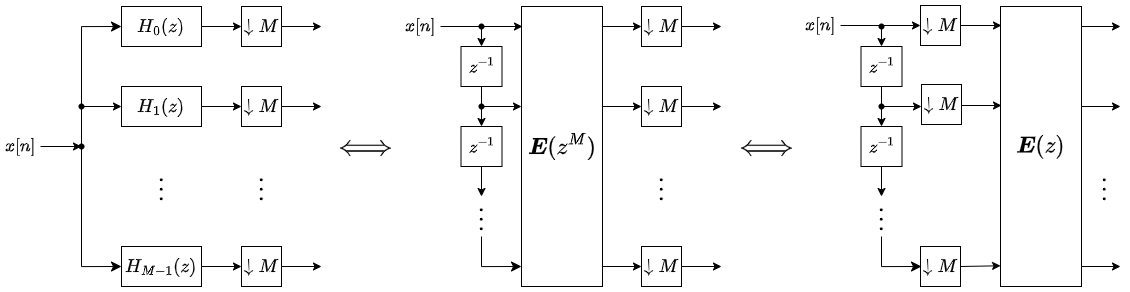
\includegraphics[width=118mm]{./figs/polyphase_representation_analyzer.drawio.png}
    \end{figure}
    \hrule
    \begin{figure}
        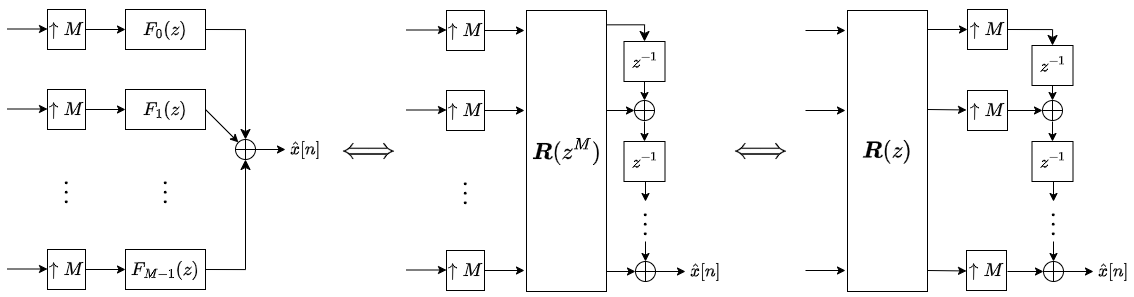
\includegraphics[width=118mm]{./figs/polyphase_representation_synthesizer.drawio.png}
    \end{figure}
\end{frame}

\begin{frame}[c]
    \frametitle{ポリフェーズ行列表現}
    $\ve{E}(z), \ve{R}(z)$により,$M$分割フィルタバンクは以下のように表せる
    \vspace{-13pt}
    \begin{figure}
        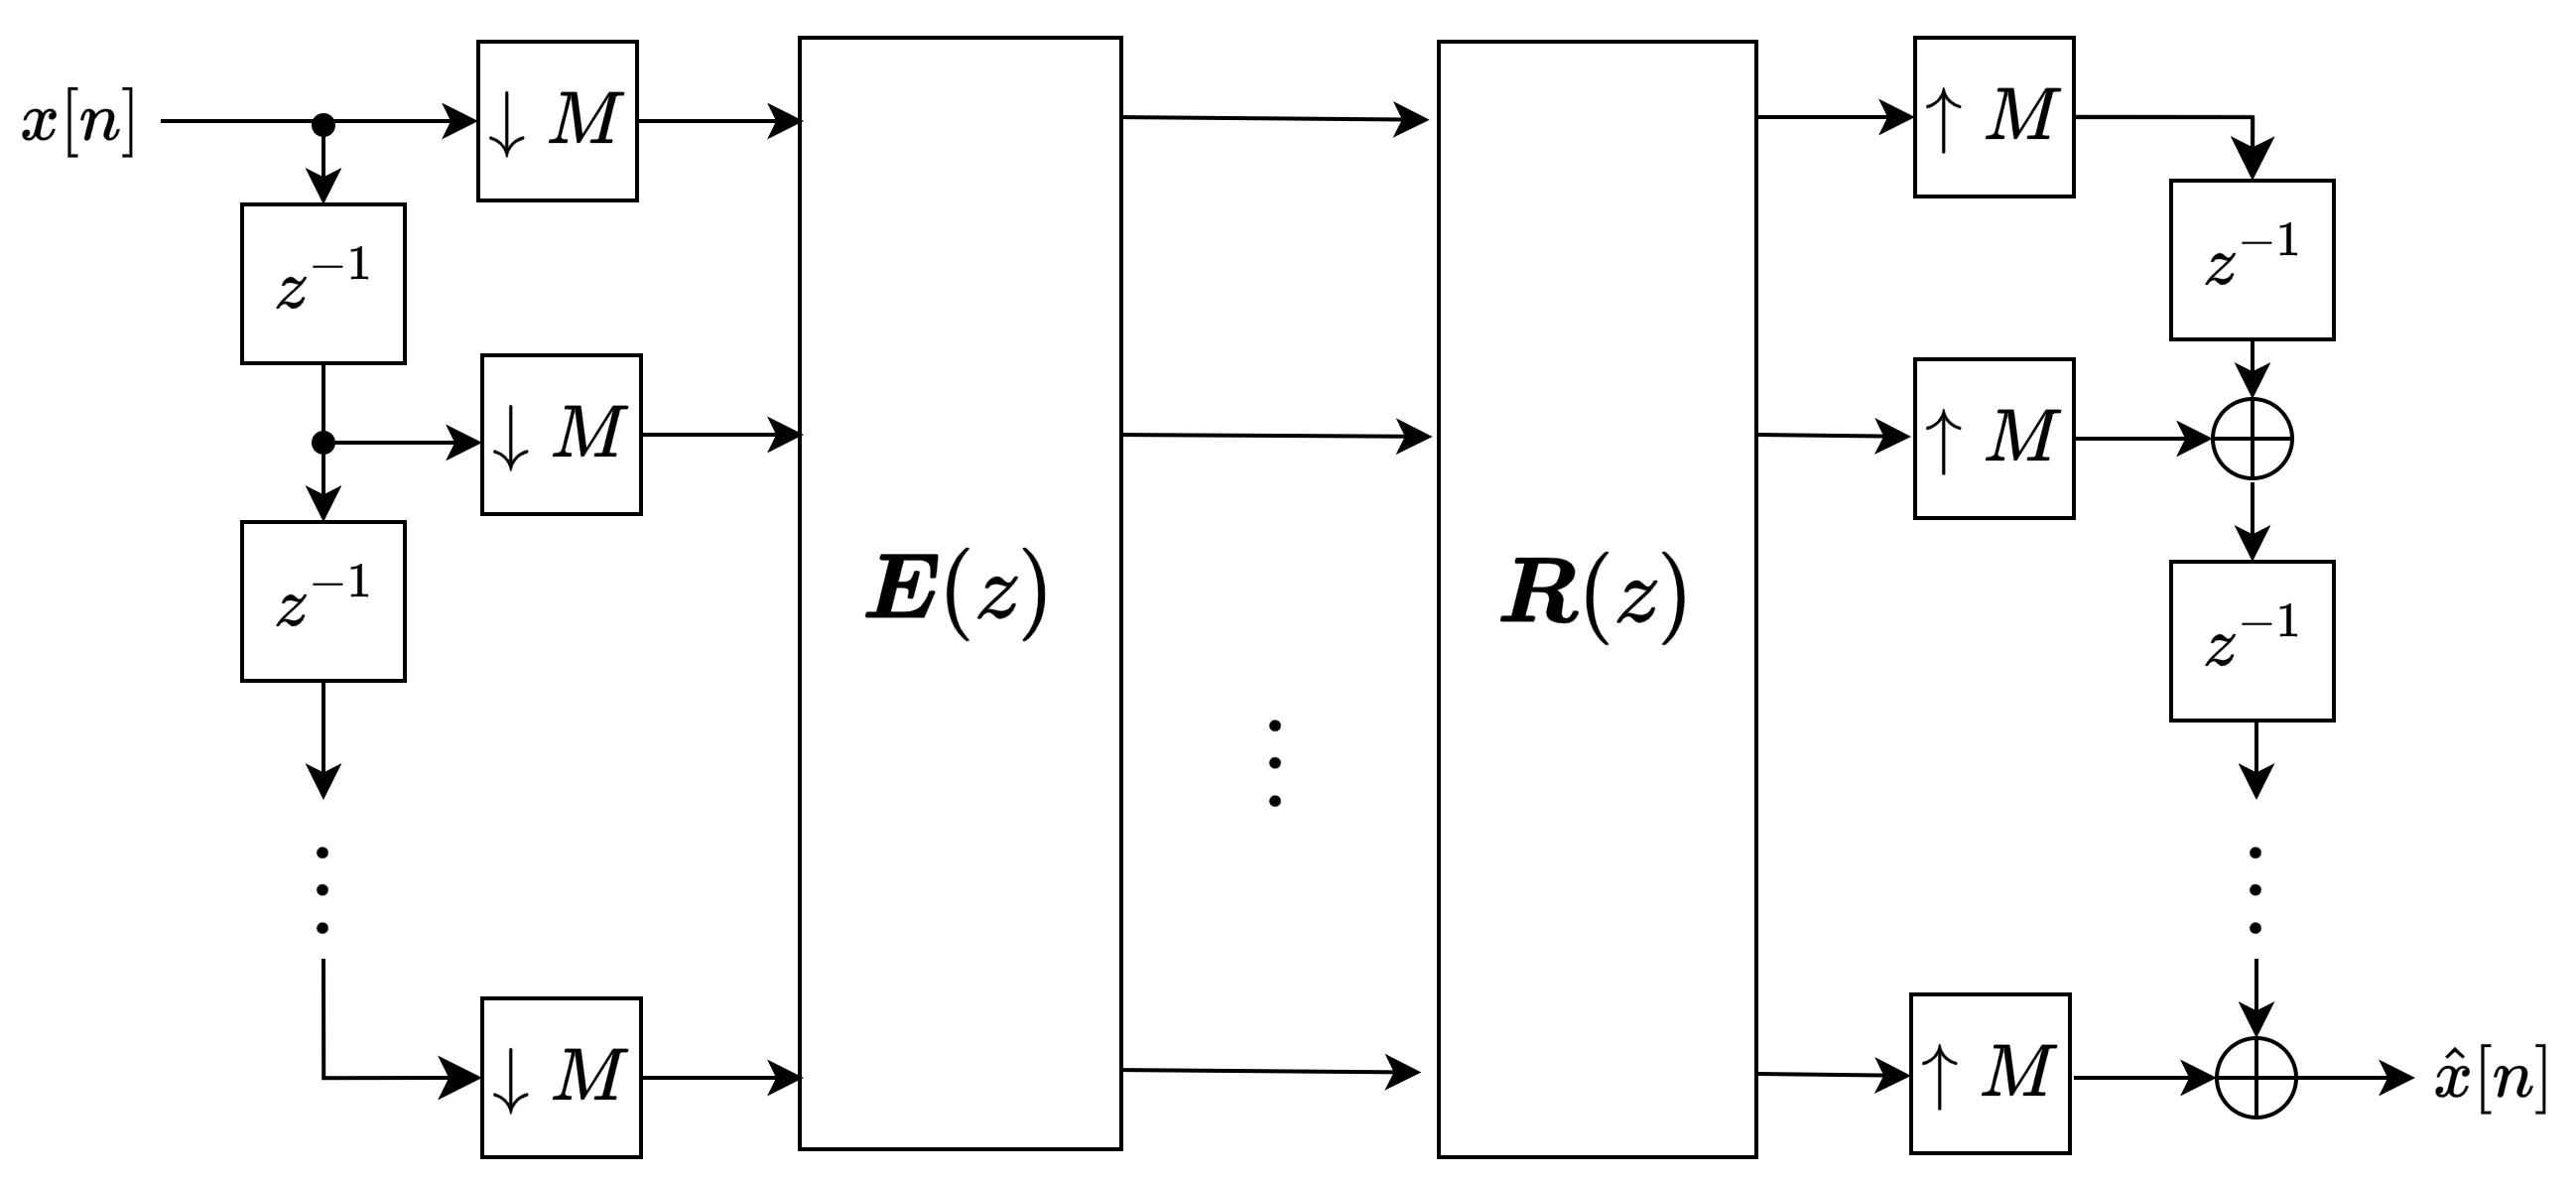
\includegraphics[width=120mm]{./figs/polyphase_representation_filter_bank.drawio.png}
    \end{figure}
\end{frame}

\begin{frame}[c]
    \frametitle{\scalebox{0.95}{完全再構成$M$分割フィルタバンク}}
    \begin{block}{}
        \vspace{-14pt}
        \begin{align}
            \ve{R}(z) \ve{E}(z) = a z^{-m_{0}} \ve{I} \quad (a \neq 0,\ m_{0} \in \mathbb{N}) \label{eq:filter_bank_PR_condition}
        \end{align}
        ならば,$M$分割フィルタバンクは完全再構成\footnote{$\because$各バンドの遅延が$K$ならば,$\hat{X}(z) = aM z^{-(M - 1 + K)}X(z)$}
    \end{block}
    \begin{figure}
        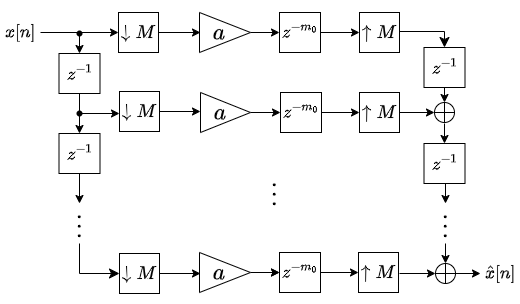
\includegraphics[width=70mm]{./figs/perfect_reconstraction_filter_bank.drawio.png}
        \caption*{$\ve{R}(z) \ve{E}(z) = a z^{-m_{0}} \ve{I}$を満たす$M$分割フィルタバンク}
    \end{figure}
\end{frame}

\begin{frame}[c]
    \frametitle{\scalebox{0.95}{完全再構成$M$分割フィルタバンク}}
    \eqref{eq:filter_bank_PR_condition}式より,$\ve{R}(z) = a z^{-m_{0}} \ve{E}(z)^{-1}$ならば完全再構成.
    \begin{itemize}
        \item しかし,$\ve{E}(z)^{-1}$の計算に問題を孕む.
    \end{itemize}
    代わりに,$\ve{E}(z)$が\structure{パラユニタリ}\footnote{$\widetilde{\ve{E}}(z) = \ve{E}_{\ast}(z^{-1})$で,下付きの$\ast$は係数の複素共役}
    \begin{align}
        \widetilde{\ve{E}}(z) \ve{E}(z) = d \ve{I}, \quad d \neq 0
    \end{align}
    ならば,
    \begin{align*}
        \ve{R}(z) = a z^{-m_{0}} \widetilde{\ve{E}}(z)
    \end{align*}
    とするとフィルタバンクは完全再構成.
\end{frame}

\begin{frame}[c]
    \frametitle{コサイン変調フィルタバンク}
    \begin{block}{}
        式\eqref{eq:cos_modulated_synthesis_filter}より,分析合成フィルタ$F_{k}(z)H_{k}(z)$は直線位相特性をもつ
    \end{block}
    \scriptsize
    (証明)
    \begin{align*}
        F_{k}(z) &= \sum_{n = -\infty}^{\infty} f_{k}[n] z^{-n} = \sum_{n = -\infty}^{\infty} h_{k}[L - 1 - n] z^{-n} \\
        &= \sum_{n^{\prime} = -\infty}^{\infty} h_{k}[n^{\prime}] z^{-(L - 1 - n^{\prime})} = z^{-(L-1)} \sum_{n^{\prime} = -\infty}^{\infty} h_{k}[n^{\prime}] z^{n^{\prime}} \\
        &= z^{-(L-1)} H_{k}(z^{-1})
    \end{align*}
    $H_{k}(z)$の周波数特性を(極座標で)$H_{k}(\omega) = |H_{k}(\omega)| \exp[j \psi(\omega)]$と書くと,
    \begin{align*}
        F_{k}(\omega) &= \exp[-j(L - 1)\omega] H_{k}(-\omega) = \exp[-j(L - 1)\omega] |H_{k}(-\omega)| \exp[-j \psi(\omega)] \\
        &= \exp[-j(L - 1)\omega] |H_{k}(\omega)| \exp[-j \psi(\omega)] \quad \text{($\because$ 実係数FIRの振幅特性は偶)}
    \end{align*}
    だから,$F_{k}(\omega) H_{k}(\omega) = \exp[-j(L - 1)\omega] |H_{k}(\omega)|^{2}$となって直線位相特性をもつ.
\end{frame}

\begin{frame}[c]
    \frametitle{コサイン変調フィルタバンク}
    $h_{k}[n]$の伝達関数を変形する.回転因子$W_{2M}$\footnote{$W_{2M} = \exp\left(-j\frac{2\pi}{2M}\right) = \exp\left(-j\frac{\pi}{M}\right)$}より
    \scriptsize
    \begin{align*}
        &\cos\left[ \frac{\pi}{M} \left( k + \frac{1}{2} \right) \left( n - \frac{L - 1}{2} \right) + \theta_{k} \right] \\
        &=
        \resizebox{\hsize}{!}{$\displaystyle
        \frac{1}{2} \left\{ \exp\left[ j \left\{ \frac{\pi}{M} \left( k + \frac{1}{2} \right) \left( n - \frac{L - 1}{2} \right) + \theta_{k} \right\} \right] + \exp\left[-j \left\{ \frac{\pi}{M} \left( k + \frac{1}{2} \right) \left( n - \frac{L - 1}{2} \right) + \theta_{k} \right\} \right] \right\}
        $}
        \\
        &= \frac{1}{2} \left\{ \exp(j\theta_{k}) W_{2M}^{\left( k + \frac{1}{2} \right)\frac{L-1}{2}}W_{2M}^{-\left( k + \frac{1}{2} \right)n} + \exp(-j\theta_{k}) W_{2M}^{-\left( k + \frac{1}{2} \right)\frac{L-1}{2}} W_{2M}^{\left( k + \frac{1}{2} \right)n} \right\}
    \end{align*}
    \normalsize
    これを\eqref{eq:cos_modulated_analysis_filter}式に代入すると,
    \scriptsize
    \begin{align*}
        H_{k}(z) &= \exp(j\theta_{k}) W_{2M}^{\left( k + \frac{1}{2} \right)\frac{L-1}{2}} \sum_{n = -\infty}^{\infty} p_{0}[n] W_{2M}^{-\left(k + \frac{1}{2} \right)n} z^{-n} \\
        &\quad + \exp(-j\theta_{k}) W_{2M}^{-\left( k + \frac{1}{2} \right)\frac{L-1}{2}} \sum_{n = -\infty}^{\infty} p_{0}[n] W_{2M}^{\left(k + \frac{1}{2} \right)n} z^{-n} \\
        &= \exp(j\theta_{k}) W_{2M}^{\left( k + \frac{1}{2} \right)\frac{L-1}{2}} P_{0}\left(W_{2M}^{k + \frac{1}{2}} z \right) + \exp(-j\theta_{k}) W_{2M}^{-\left( k + \frac{1}{2} \right)\frac{L-1}{2}} P_{0}\left(W_{2M}^{-\left(k + \frac{1}{2}\right)} z \right)
    \end{align*}
\end{frame}

\begin{frame}[c]
    \frametitle{コサイン変調フィルタバンク}
    さらに\eqref{eq:polyphase_representation_of_prototype}式を代入すると\footnote{$\left( W_{2M}^{\pm \left( k + \frac{1}{2} \right) }\right)^{2M} = \exp\left[ \mp j \frac{\pi}{M} \left( k + \frac{1}{2} \right) 2M \right] = \exp[\mp j \pi(2k + 1)] = -1$を使用}
    \scriptsize
    \begin{align*}
        &H_{k}(z) = \exp(j\theta_{k}) W_{2M}^{\left( k + \frac{1}{2} \right)\frac{L-1}{2}} \sum_{l = 0}^{2M - 1} \left( W_{2M}^{k + \frac{1}{2}} z \right)^{-l} G_{l}\left( \left( W_{2M}^{k + \frac{1}{2}} z \right)^{2M} \right) \\
        &\quad\quad\quad + \exp(-j\theta_{k}) W_{2M}^{-\left( k + \frac{1}{2} \right)\frac{L-1}{2}} \sum_{l = 0}^{2M - 1} \left( W_{2M}^{-\left( k + \frac{1}{2} \right)} z \right)^{-l} G_{l}\left( \left( W_{2M}^{-\left( k + \frac{1}{2} \right)} z \right)^{2M} \right) \\
        &= \exp(j\theta_{k}) W_{2M}^{\left( k + \frac{1}{2} \right)\frac{L-1}{2}} \sum_{l = 0}^{2M - 1} W_{2M}^{-l\left( k + \frac{1}{2} \right)} z^{-l} G_{l}(-z^{2M}) \\
        &\quad\quad\quad + \exp(-j\theta_{k}) W_{2M}^{-\left( k + \frac{1}{2} \right)\frac{L-1}{2}} \sum_{l = 0}^{2M - 1} W_{2M}^{l\left( k + \frac{1}{2} \right)} z^{-l} G_{l}(-z^{2M}) \\
        &=
        \scalebox{0.97}{$\displaystyle\sum_{l = 0}^{2M - 1} \left\{ \exp(j\theta_{k}) W_{2M}^{\left( k + \frac{1}{2} \right)\frac{L-1}{2}} W_{2M}^{-l\left( k + \frac{1}{2} \right)} + \exp(-j\theta_{k}) W_{2M}^{-\left( k + \frac{1}{2} \right)\frac{L-1}{2}}W_{2M}^{l\left( k + \frac{1}{2} \right)} \right\} z^{-l} G_{l}(-z^{2M})$}
        \\
        &= \sum_{l = 0}^{2M - 1} 2 \cos\left[ \frac{\pi}{M} \left( k + \frac{1}{2} \right) \left( l - \frac{L - 1}{2} \right) + \theta_{k} \right] z^{-l} G_{l}(-z^{2M})
    \end{align*}
\end{frame}

\begin{frame}[c]
    \frametitle{コサイン変調フィルタバンク}
    さらに変形すると
    \small
    \begin{align}
        H_{k}(z) &= \sum_{l = 0}^{M - 1} z^{-l} \left\{ t_{k,l} G_{l}(-z^{2M}) + z^{-M} t_{k,M + l} G_{M + l}(-z^{2M}) \right\} \label{eq:another_polyphase_representation} \\
        t_{k,l} &:= 2\cos\left[ \frac{\pi}{M} \left( k + \frac{1}{2} \right) \left( l - \frac{L - 1}{2} \right) + \theta_{k} \right] \nonumber
    \end{align}
    \normalsize
    \eqref{eq:type1_polyphase_representation}式と\eqref{eq:another_polyphase_representation}式を見比べると,
    \begin{align}
        E_{k, l}(z) = t_{k,l} G_{l}(-z^{2}) + z^{-1} t_{k,M + l} G_{M + l}(-z^{2}) \label{eq:polyphase_representation_of_cos_modulated_filter_bank}
    \end{align}
\end{frame}

\begin{frame}[c]
    \frametitle{コサイン変調フィルタバンク}
    \eqref{eq:polyphase_representation_of_cos_modulated_filter_bank}式より,アナライザのポリフェーズ行列は,
    \footnotesize
    \begin{align}
        \ve{E}(z) &=
        \underbrace{\begin{bNiceMatrix}[margin, nullify-dots, xdots/shorten=0.5em]
            t_{0,0} & \Cdots &   t_{0,2M-1} \\
            t_{1,0} & \Cdots &   t_{1,2M-1} \\
            \Vdots & \Cdots &      \Vdots  \\
            t_{M-1,0} & \Cdots & t_{M-1,2M-1} \\
        \end{bNiceMatrix}}_{\ve{T}}
        \begin{bNiceMatrix}[margin, nullify-dots, xdots/shorten=0.5em]
            G_{0}(-z^{2}) &        &                         \\
            & \Ddots &                         \\
            &        &         G_{M-1}(-z^{2}) \\
            z^{-1}G_{M}(-z^{2}) &        &                         \\
            & \Ddots &                         \\
            &        & z^{-1} G_{2M-1}(-z^{2}) \\
        \end{bNiceMatrix}
        \nonumber \\
        &= \ve{T}
        \begin{bNiceMatrix}[margin, nullify-dots, xdots/shorten=0.5em]
            \ve{G}_{0}(z^{2}) \\
            z^{-1} \ve{G}_{1}(z^{2}) \\
        \end{bNiceMatrix} \label{eq:analyzer_matrix_of_cos_modulated_filter_bank} \\
        \ve{G}_{i}(z) &:=
        \diag \begin{bNiceMatrix}[margin, nullify-dots, xdots/shorten=0.5em]
            G_{Mi}(-z) & G_{Mi + 1}(-z) & \Cdots & G_{Mi + M - 1}(-z)
        \end{bNiceMatrix}
    \end{align}
    \normalsize
    と書ける
\end{frame}

\begin{frame}[c]
    \frametitle{コサイン変調フィルタバンク}
    シンセサイザを構成する.フィルタ係数は実だから,
    \begin{align}
        \widetilde{\ve{E}}(z) = \ve{E}_{\ast}(z^{-1})^{\mathsf{T}} =
        \begin{bNiceMatrix}[margin, nullify-dots, xdots/shorten=0.5em]
            \ve{G}_{0}(z^{-1}) & z \ve{G}_{1}(z^{-1})
        \end{bNiceMatrix}
        \ve{T}^{\mathsf{T}}
    \end{align}
    $G_{l}(z)$の次数は$2K - 1$で,因果性のためには$2K - 1$の遅延がいるため
    \begin{align}
        \ve{R}(z) &= z^{-(2K-1)} \widetilde{\ve{E}}(z) \nonumber \\
        &=
        z^{-(2K-1)}
        \begin{bNiceMatrix}[margin, nullify-dots, xdots/shorten=0.5em]
            \ve{G}_{0}(z^{-1}) & z \ve{G}_{1}(z^{-1})
        \end{bNiceMatrix}
        \ve{T}^{\mathsf{T}} \label{eq:synthesizer_matrix_of_cos_modulated_filter_bank}
    \end{align}
\end{frame}

\begin{frame}[c]
    \frametitle{コサイン変調フィルタバンク}
    \begin{figure}
        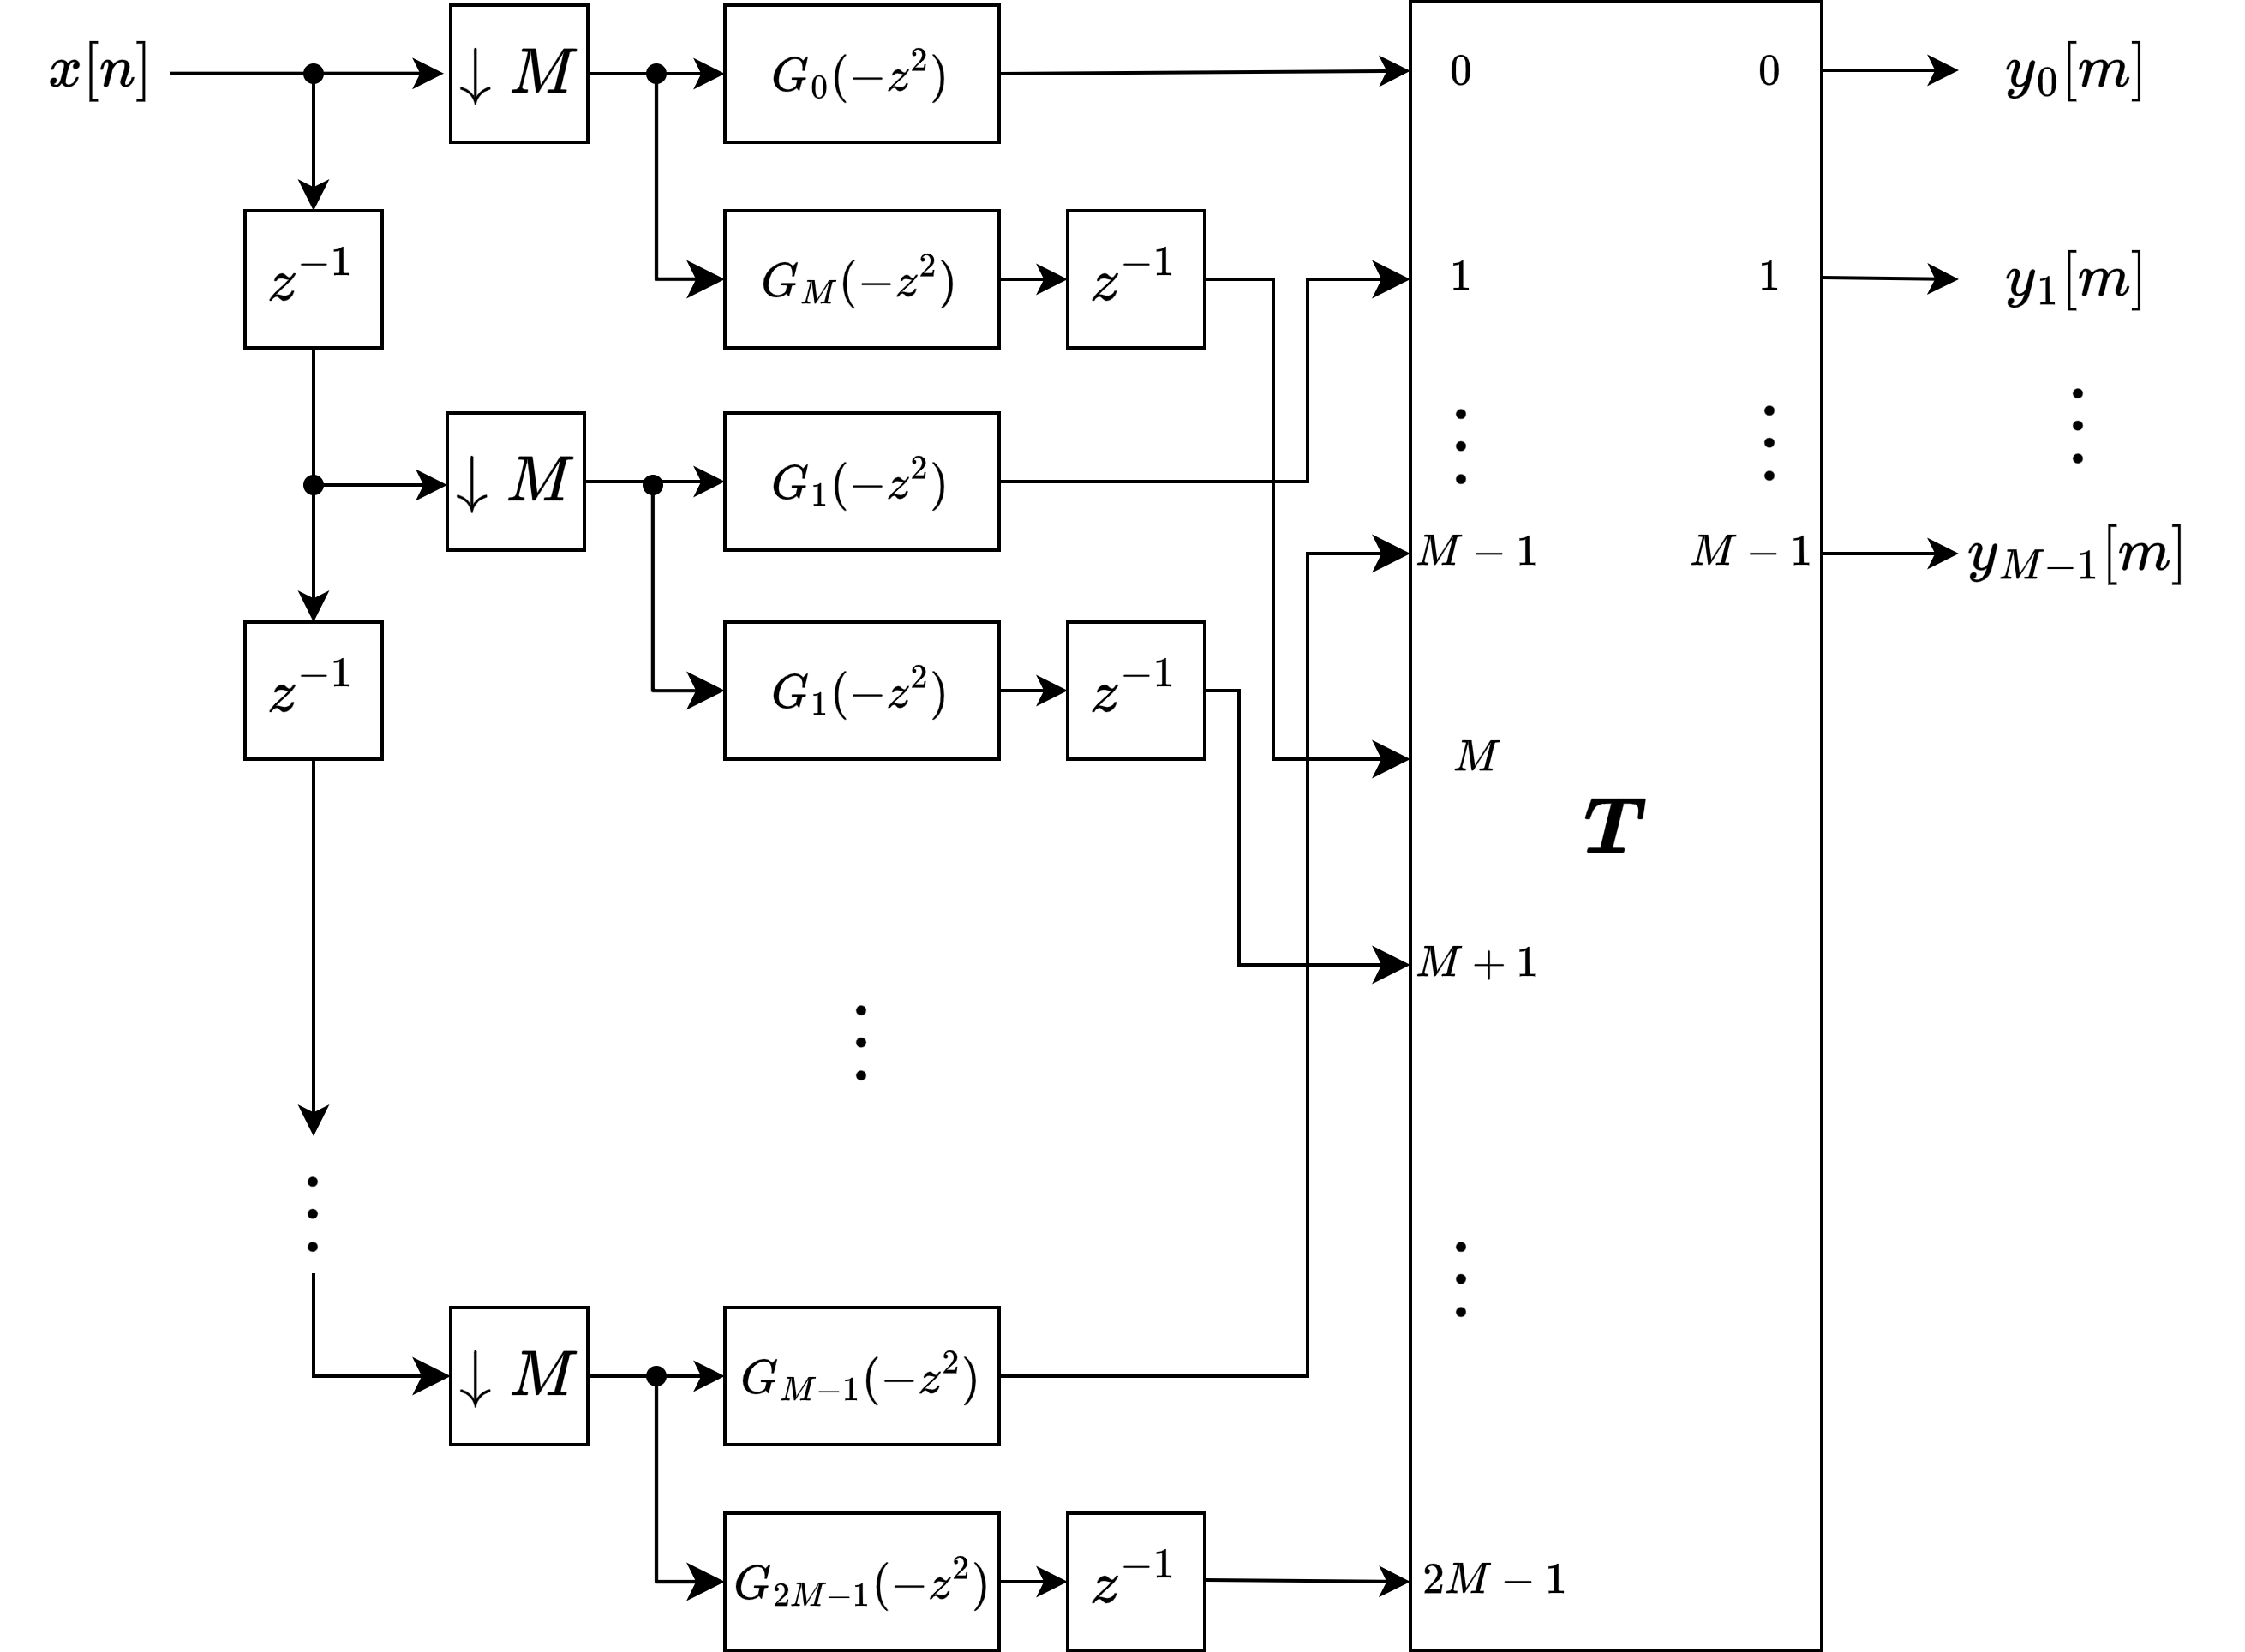
\includegraphics[width=103mm]{./figs/cos_modulated_analysis_bank_filter.drawio.png}
        \caption*{アナライザの構成}
    \end{figure}
\end{frame}

\begin{frame}[c]
    \frametitle{コサイン変調フィルタバンク}
    \begin{figure}
        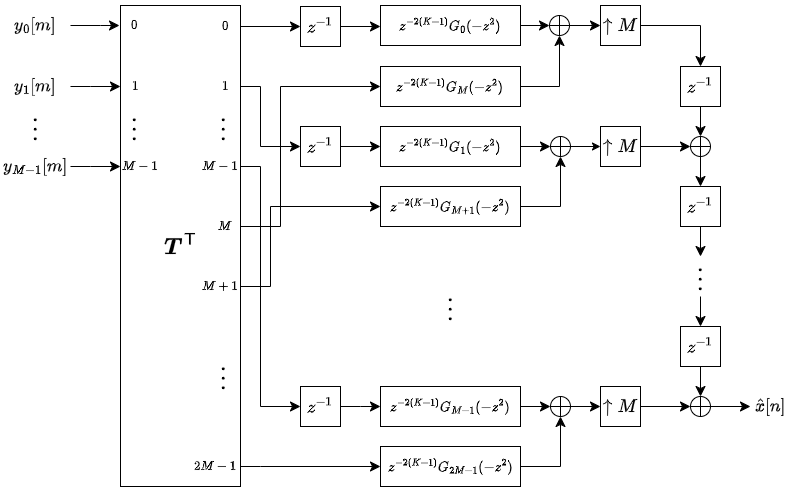
\includegraphics[width=117mm]{./figs/cos_modulated_synthesis_bank_filter.drawio.png}
        \caption*{シンセサイザの構成}
    \end{figure}
\end{frame}

\begin{frame}[c]
    \frametitle{コサイン変調フィルタバンク}
    完全再構成条件を導く.\eqref{eq:analyzer_matrix_of_cos_modulated_filter_bank},\eqref{eq:synthesizer_matrix_of_cos_modulated_filter_bank}式より,
    \begin{align*}
        & \ve{R}(z)\ve{E}(z) = z^{-(2K - 1)} \widetilde{\ve{E}}(z) \ve{E}(z) \\
        &= z^{-(2K - 1)}
        \begin{bNiceMatrix}[margin, nullify-dots, xdots/shorten=0.5em]
            \ve{G}_{0}(z^{-1}) & z \ve{G}_{1}(z^{-1})
        \end{bNiceMatrix}
        \ve{T}^{\mathsf{T}} \ve{T}
        \begin{bNiceMatrix}[margin, nullify-dots, xdots/shorten=0.5em]
            \ve{G}_{0}(z) \\
            z^{-1} \ve{G}_{1}(z)
        \end{bNiceMatrix} \\
        &= 2M z^{-(2K - 1)} \left\{ \ve{G}_{0}(z^{-1}) \ve{G}_{0}(z) + \ve{G}_{1}(z^{-1}) \ve{G}_{1}(z) \right\}
    \end{align*}
    ここで,$\ve{T}^{\mathsf{T}} \ve{T} = 2M \ve{I}$(後で示す).$\ve{G}_{0}, \ve{G}_{1}$は対角行列だから,$k = 0, ..., M-1$に対し,
    \begin{align*}
        G_{k}(z^{-1}) G_{k}(z) + G_{M + k}(z^{-1}) G_{M + k}(z) = \alpha
    \end{align*}
    を満たせば完全再構成となる
\end{frame}

\begin{frame}[c]
    \frametitle{コサイン変調フィルタバンク}
    \begin{block}{コサイン変調フィルタバンクの完全再構成条件}
        $k = 0, ..., M-1$に対し,定数$\alpha \in \mathbb{R}$があって
        \begin{align}
            G_{k}(z^{-1}) G_{k}(z) + G_{M + k}(z^{-1}) G_{M + k}(z) = \alpha
        \end{align}
        となること.ここで,
        \begin{align}
            G_{k}(z) = \sum_{n = -\infty}^{\infty} p_{0}[2Mn + k] z^{-n} \label{eq:polyphase_representation_of_prototype}
        \end{align}
        $G_{k}(z)$は$p_{0}[n]$のポリフェーズ表現
    \end{block}
    本条件は\structure{電力相補条件}ともいう
\end{frame}

\begin{frame}[c]
    \frametitle{$\ve{T}^{\mathsf{T}} \ve{T} = 2M\ve{I}$の証明}
    $\left( \ve{T}^{\mathsf{T}} \ve{T} \right)_{ij} = \sum_{k = 0}^{M - 1} t_{k,i} t_{k,j}$であり,
    \scriptsize
    \begin{align*}
        & t_{k,i} t_{k,j} \\
        &= 4 \cos\left[ \frac{\pi}{M} \left( k + \frac{1}{2} \right) \left( i - \frac{L - 1}{2} \right) + (-1)^{k}\frac{\pi}{4} \right] \cos\left[ \frac{\pi}{M} \left( k + \frac{1}{2} \right) \left( j - \frac{L - 1}{2} \right) + (-1)^{k}\frac{\pi}{4} \right] \\
        &= 2 \left\{ \cos\left[ \frac{\pi}{M} \left( k + \frac{1}{2} \right) \left\{ i + j - (L - 1) \right\} + (-1)^{k} \frac{\pi}{2} \right] + \cos\left[ \frac{\pi}{M} \left( k + \frac{1}{2} \right) \left( i - j \right) \right] \right\}
    \end{align*}
    \normalsize
    $i + j - (L - 1) = A$とおくと,
    \scriptsize
    \begin{align*}
        & \cos\left[ \frac{\pi}{M} \left( k + \frac{1}{2} \right)A + (-1)^{k}\frac{\pi}{2} \right] \\
        &= \cos\left[ \frac{\pi}{M} \left( k + \frac{1}{2} \right)A \right] \cos\left[(-1)^{k}\frac{\pi}{2} \right] - \sin\left[ \frac{\pi}{M} \left( k + \frac{1}{2} \right)A \right] \sin\left[(-1)^{k}\frac{\pi}{2} \right] \\
        &= -(-1)^{k} \sin \left[ \frac{\pi}{M} \left( k + \frac{1}{2} \right)A \right]
    \end{align*}
\end{frame}

\begin{frame}[c]
    \frametitle{$\ve{T}^{\mathsf{T}} \ve{T} = 2M\ve{I}$の証明}
    ここで,
    \begin{align}
        \sum_{k = 0}^{M - 1}\cos\left[ \frac{\pi}{M} \left( k + \frac{1}{2} \right) \left( i - j \right) \right] &= M\delta_{ij} \label{eq:orthogonal_condition_cos} \\
        \sum_{k = 0}^{M - 1}(-1)^{k} \sin \left[ \frac{\pi}{M} \left( k + \frac{1}{2} \right)A \right] &= 0 \label{eq:orthogonal_condition_sin}
    \end{align}
    ($\delta_{ij}$:クロネッカーのデルタ)を示せば,
    \begin{align*}
        \left( \ve{T}^{\mathsf{T}} \ve{T} \right)_{ij} = 2M \delta_{ij}
    \end{align*}
    となり命題が示せる.次ページから計算結果を載せる
\end{frame}

\begin{frame}[c]
    \frametitle{$\ve{T}^{\mathsf{T}} \ve{T} = 2M\ve{I}$の証明}
    \eqref{eq:orthogonal_condition_cos}式を示す.$i = j$のとき,
    \scriptsize
    $\sum_{k = 0}^{M - 1} \cos\left[ \frac{\pi}{M} \left( k + \frac{1}{2} \right) ( i - j ) \right] = M$.
    \normalsize
    $i \neq j$のとき,
    \scriptsize
    \begin{align*}
        & \sum_{k = 0}^{M - 1} \cos\left[ \frac{\pi}{M} \left( k + \frac{1}{2} \right) ( i - j ) \right] \\
        &= \frac{1}{2} \sum_{k = 0}^{M - 1} \left\{ \exp\left[ j \frac{\pi}{M}  \left( k + \frac{1}{2} \right) (i - j) \right] + \exp\left[ -j \frac{\pi}{M} \left( k + \frac{1}{2} \right) (i - j) \right] \right\} \\
        &= \frac{1}{2} \sum_{k = 0}^{M - 1} \left\{ W_{2M}^{-\left( k + \frac{1}{2} \right)(i - j)} + W_{2M}^{\left( k + \frac{1}{2} \right)(i - j)} \right\} \nonumber \\
        &= \frac{1}{2} \left\{ W_{2M}^{-\frac{i - j}{2}} \sum_{k = 0}^{M - 1} W_{2M}^{-(i - j)k} + W_{2M}^{\frac{i - j}{2}} \sum_{k = 0}^{M - 1} W_{2M}^{(i - j)k} \right\} \\
        &= \frac{1}{2} \left[ \frac{W_{2M}^{-\frac{i - j}{2}}}{W_{2M}^{-(i - j)} - 1} \left\{ (-1)^{-(i - j)} - 1 \right\} + \frac{W_{2M}^{\frac{i - j}{2}}}{W_{2M}^{i - j} - 1} \left\{ (-1)^{i - j} - 1 \right\} \right]
    \end{align*}
    最後の式変形で等比級数の和$\sum_{k = 0}^{M - 1} W_{2M}^{(i - j)k} = \frac{W_{2M}^{(i -j)M} - 1}{W_{2M}^{i - j} - 1} = \frac{(-1)^{i - j} - 1}{W_{2M}^{i - j} - 1}$を使用
\end{frame}

\begin{frame}[c]
    \frametitle{$\ve{T}^{\mathsf{T}} \ve{T} = 2M\ve{I}$の証明}
    さらに式変形すると,
    \scriptsize
    \begin{align*}
        & \sum_{k = 0}^{M - 1} \cos\left[ \frac{\pi}{M} \left( k + \frac{1}{2} \right) ( i - j ) \right] \\
        &= \frac{1}{2} \left[ \frac{W_{2M}^{-\frac{i - j}{2}}}{W_{2M}^{-(i - j)} - 1} \left\{ (-1)^{-(i - j)} - 1 \right\} + \frac{W_{2M}^{\frac{i - j}{2}}}{W_{2M}^{i - j} - 1} \left\{ (-1)^{i - j} - 1 \right\} \right] \\
        &= \frac{W_{2M}^{-\frac{i - j}{2}} (W_{2M}^{i - j} - 1)\left\{ (-1)^{-(i - j)} - 1 \right\} + W_{2M}^{\frac{i - j}{2}} (W_{2M}^{-(i - j)} - 1)\left\{ (-1)^{i - j} - 1 \right\}}{2(W_{2M}^{-(i - j)} - 1)(W_{2M}^{i - j} - 1)} \\
        &= \frac{(W_{2M}^{\frac{i - j}{2}} - W_{2M}^{-\frac{i - j}{2}})\left\{ (-1)^{-(i - j)} - 1 \right\} + (W_{2M}^{-\frac{i - j}{2}} - W_{2M}^{\frac{i - j}{2}})\left\{ (-1)^{i - j} - 1 \right\}}{2(W_{2M}^{-(i - j)} - 1)(W_{2M}^{i - j} - 1)} \\
        &= \frac{(W_{2M}^{\frac{i - j}{2}} - W_{2M}^{-\frac{i - j}{2}})\left\{ (-1)^{i - j} - 1 \right\} + (W_{2M}^{-\frac{i - j}{2}} - W_{2M}^{\frac{i - j}{2}})\left\{ (-1)^{i - j} - 1 \right\}}{2(W_{2M}^{-(i - j)} - 1)(W_{2M}^{i - j} - 1)} \\
        &= 0
    \end{align*}
    \normalsize
    よって\eqref{eq:orthogonal_condition_cos}式が示された
\end{frame}

\begin{frame}[c]
    \frametitle{$\ve{T}^{\mathsf{T}} \ve{T} = 2M\ve{I}$の証明}
    \eqref{eq:orthogonal_condition_sin}式を示す.
    \scriptsize
    \begin{align*}
        & \sum_{k = 0}^{M - 1} (-1)^{k} \sin\left[ \frac{\pi}{M} \left( k + \frac{1}{2} \right) A  \right] \\
        &= \frac{1}{j2} \sum_{k = 0}^{M - 1} (-1)^{k} \left\{ \exp\left[ j \frac{\pi}{M} \left( k + \frac{1}{2} \right) A  \right] - \exp\left[ -j \frac{\pi}{M} \left( k + \frac{1}{2} \right) A  \right] \right\} \\
        &= \frac{1}{j2} \sum_{k = 0}^{M - 1} (-1)^{k} \left\{ W_{2M}^{-A\left( k + \frac{1}{2} \right)} - W_{2M}^{A\left( k + \frac{1}{2} \right)} \right\} \\
        &= \frac{1}{j2} \left\{ W_{2M}^{-\frac{A}{2}} \sum_{k = 0}^{M - 1} (-1)^{k} W_{2M}^{-Ak} - W_{2M}^{\frac{A}{2}} \sum_{k = 0}^{M - 1} (-1)^{k} W_{2M}^{Ak} \right\} \\
        &= \frac{1}{j2} \left\{ W_{2M}^{-\frac{A}{2}} \sum_{k = 0}^{M - 1} W_{2M}^{-(M + A)k} - W_{2M}^{\frac{A}{2}} \sum_{k = 0}^{M - 1} W_{2M}^{(M + A)k} \right\} \quad \text{($\because$ $(-1)^{k} = W_{2M}^{M} = W_{2M}^{-M}$)} \\
        &= \frac{1}{j2} \left\{ W_{2M}^{-\frac{A}{2}} \frac{(-1)^{-(M + A)} - 1}{W_{2M}^{-(M + A)} - 1} - W_{2M}^{\frac{A}{2}} \frac{(-1)^{M + A} - 1}{W_{2M}^{M + A} - 1} \right\} \quad \text{($\because$ 等比級数の和の公式)}
    \end{align*}
\end{frame}

\begin{frame}[c]
    \frametitle{$\ve{T}^{\mathsf{T}} \ve{T} = 2M\ve{I}$の証明}
    さらに計算を進めると,
    \scriptsize
    \begin{align*}
        & \sum_{k = 0}^{M - 1} (-1)^{k} \sin\left[ \frac{\pi}{M} \left( k + \frac{1}{2} \right) A \right] \\
        &= \frac{W_{2M}^{-\frac{A}{2}} \left\{ (-1)^{-(M + A)} - 1 \right\} (W_{2M}^{M + A} - 1) - W_{2M}^{\frac{A}{2}} \left\{ (-1)^{M + A} - 1 \right\} (W_{2M}^{-(M + A)} - 1)}{j2(W_{2M}^{-(M + A)} - 1)(W_{2M}^{(M + A)} - 1)} \\
        &= \frac{\left\{(-1)^{M + A} - 1 \right\}\left\{ W_{2M}^{-\frac{A}{2}} ( W_{2M}^{M + A} - 1 ) - W_{2M}^{\frac{A}{2}} ( W_{2M}^{-(M + A)} - 1 )\right\}}{j2(W_{2M}^{-(M + A)} - 1)(W_{2M}^{(M + A)} - 1)} \\
        &= \frac{\left\{(-1)^{M + A} - 1 \right\}\left( W_{2M}^{M + \frac{A}{2}} - W_{2M}^{-\frac{A}{2}} - W_{2M}^{-M - \frac{A}{2}} + W_{2M}^{\frac{A}{2}} \right)}{j2(W_{2M}^{-(M + A)} - 1)(W_{2M}^{(M + A)} - 1)} \\
        &= \frac{\left\{(-1)^{M + A} - 1 \right\}\left( -W_{2M}^{\frac{A}{2}} - W_{2M}^{-\frac{A}{2}} + W_{2M}^{-\frac{A}{2}} + W_{2M}^{\frac{A}{2}} \right)}{j2(W_{2M}^{-(M + A)} - 1)(W_{2M}^{(M + A)} - 1)} \\
        &= 0
    \end{align*}
    \normalsize
    よって,\eqref{eq:orthogonal_condition_sin}式が示された.
\end{frame}

\begin{frame}[c]
    \frametitle{MP3のフィルタバンクの特性}
    \vspace{-5pt}
    \begin{figure}
        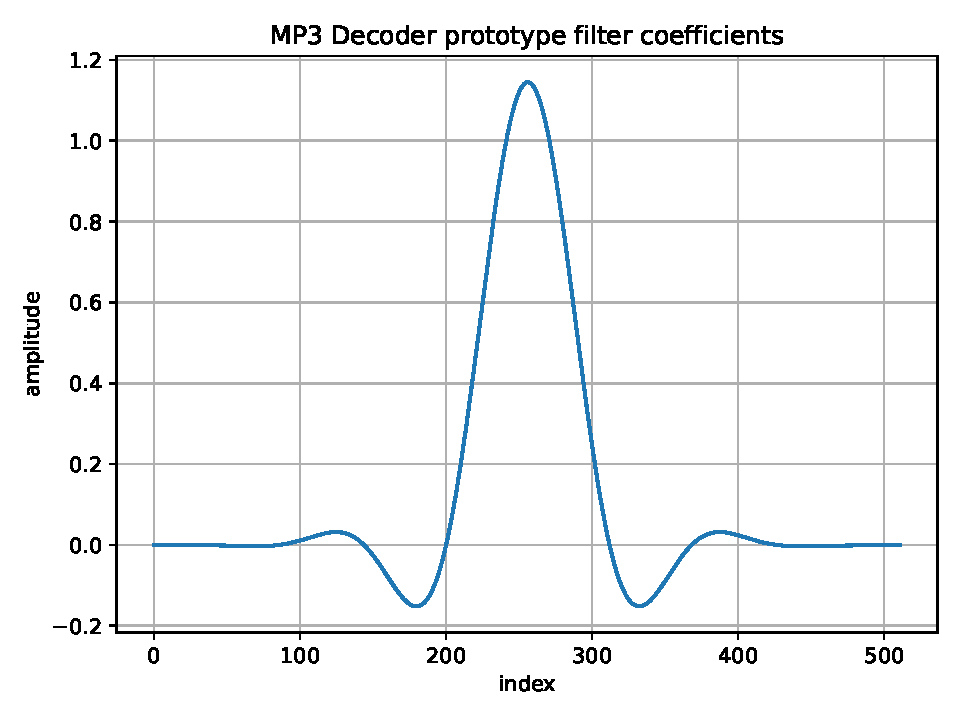
\includegraphics[width=100mm]{./figs/mp3_decoder_prototype_filter_coef.pdf}
    \end{figure}
    \vspace{-5pt}
    \begin{itemize}
        \item デコーダの係数.エンコーダの係数の$32$倍
    \end{itemize}
\end{frame}

\begin{frame}[c]
    \frametitle{電力相補条件の確認}
    MP3のフィルタバンクでは
    \scriptsize
    \begin{align*}
        & G_{k}(z) = \sum_{n = -\infty}^{\infty} p_{0}[2nM + k] z^{-n} = \sum_{n = 0}^{7} p_{0}[64n + k] z^{-n} = \sum_{n = 0}^{7} (-1)^{n} C_{64 + k} z^{-n} \\
        & G_{M+k}(z) = \sum_{n = 0}^{7} p_{0}[64n + 32 + k] z^{-n} = \sum_{n = 0}^{7} (-1)^{n} C_{64n + 32 + k} z^{-n} \\
        & G_{k}(z^{-1}) = \sum_{n = -\infty}^{\infty} p_{0}[64n + k] (z^{-1})^{-n} = \sum_{n = -\infty}^{\infty} p_{0}[-64n + k] z^{-n} = \sum_{n = -7}^{0} (-1)^{n} C_{-64n + k} z^{-n} \\
        & G_{M+k}(z^{-1}) = \sum_{n = 0}^{7} p_{0}[-64n + 32 + k] z^{-n} = \sum_{n = 0}^{7} (-1)^{n} C_{-64n + 32 + k} z^{-n}
    \end{align*}
    \normalsize
    $k = 0, ..., 31$で実際に計算すると,
    \begin{align*}
        G_{k}(z^{-1})G_{k}(z) + G_{M+k}(z^{-1})G_{M+k}(z) \approx \frac{1}{512}
    \end{align*}
\end{frame}

\begin{frame}[c]
    \frametitle{電力相補条件の確認(計算結果)}
    \begin{figure}
        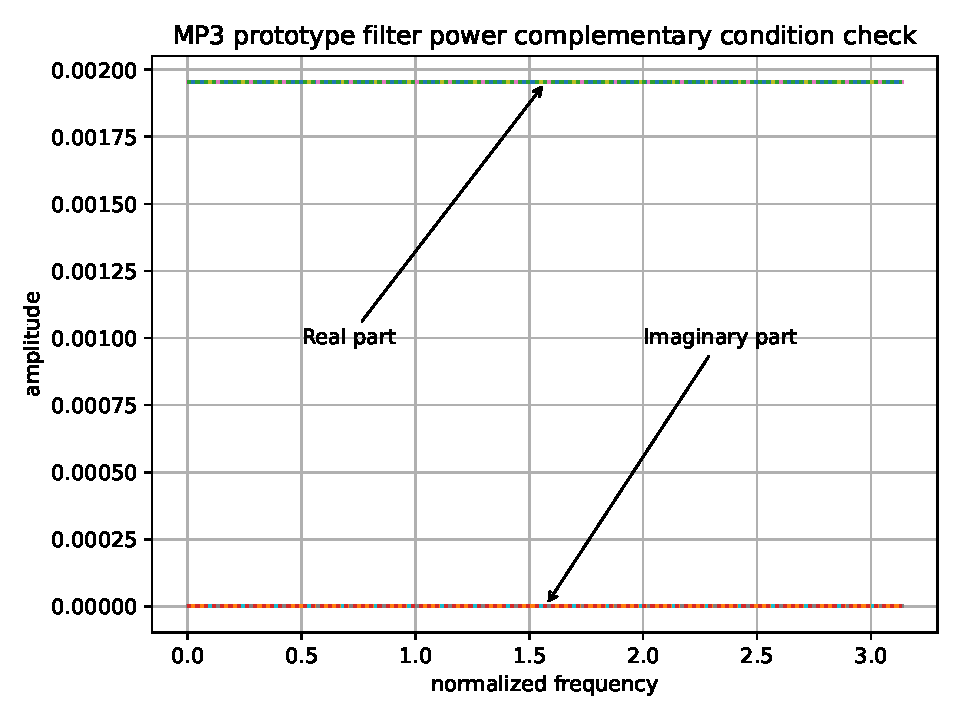
\includegraphics[width=100mm]{./figs/mp3_encoder_prototype_filter_power_complementary_condition.pdf}
    \end{figure}
    \vspace{-10pt}
    "ほぼ"完全再構成と言ってよい
\end{frame}

\subsection{MDCT} \label{sec:proofs_mdct}

\begin{frame}[c]
    \frametitle{MDCT・IMDCTによる再構成信号}
    式\eqref{eq:imdct}に式\eqref{eq:mdct}を代入すると,
    \scriptsize
    \begin{align*}
        y[n] &= \frac{2}{N} \sum_{k = 0}^{N - 1} \sum_{m = 0}^{2N - 1} x[m] \cos \left[ \frac{\pi}{N} \left( k + \frac{1}{2} \right) \left( m + \frac{1}{2} + \frac{N}{2} \right) \right] \cos \left[ \frac{\pi}{N} \left( k + \frac{1}{2} \right) \left( n + \frac{1}{2} + \frac{N}{2} \right) \right] \\
        &= \frac{1}{N} \sum_{k = 0}^{N - 1} \sum_{m = 0}^{2N - 1} x[m] \left\{ \cos \left[ \frac{\pi}{N} \left( k + \frac{1}{2} \right) \left( n + m + 1 + N \right) \right] + \cos \left[ \frac{\pi}{N} \left( k + \frac{1}{2} \right) \left( n - m \right) \right] \right\} \\
        &= \frac{1}{N} \sum_{m = 0}^{2N - 1} x[m] \sum_{k = 0}^{N - 1} \left\{ \cos \left[ \frac{\pi}{N} \left( k + \frac{1}{2} \right) \left( n + m + 1 + N \right) \right] + \cos \left[ \frac{\pi}{N} \left( k + \frac{1}{2} \right) \left( n - m \right) \right] \right\}
    \end{align*}
    \normalsize
    ここで,
    \begin{align}
        I_{n} := \sum_{k = 0}^{N - 1} \cos \left[ \frac{\pi}{N} \left( k + \frac{1}{2} \right) n \right]
    \end{align}
    を計算していく
\end{frame}

\begin{frame}[c]
    \frametitle{MDCT・IMDCTによる再構成信号}
    \scriptsize
    \begin{align*}
        I_{n} &= \sum_{k = 0}^{N - 1} \cos \left[ \frac{\pi}{N} \left( k + \frac{1}{2} \right) n \right] = \sum_{k = 0}^{N - 1} \cos \left[ \frac{\pi}{2N} ( 2k + 1 ) n \right] \\
        &= \frac{1}{2} \sum_{k = 0}^{N - 1} \left\{ \exp\left[ j \frac{\pi}{2N} ( 2k + 1 )n \right] + \exp\left[-j \frac{\pi}{2N} ( 2k + 1 )n \right] \right\} \\
        &= \frac{1}{2} \sum_{k = 0}^{N - 1} \left( W_{2N}^{-\frac{2k + 1}{2}n} + W_{2N}^{\frac{2k + 1}{2}n} \right) = \frac{1}{2} \left( W_{2N}^{-\frac{n}{2}} \sum_{k = 0}^{N - 1} W_{2N}^{-nk} + W_{2N}^{\frac{n}{2}} \sum_{k = 0}^{N - 1} W_{2N}^{nk} \right)
    \end{align*}
    ここで,
    \begin{align*}
        \sum_{k = 0}^{N - 1} W_{2N}^{nk} &= \sum_{k = 0}^{N - 1} \left( W_{2N}^{n} \right)^{k}
        = \left\{ \begin{array}{ll}
            \displaystyle \sum_{k = 0}^{N - 1} 1^{k} = N & \text{($n$が$2N$の倍数)} \\
            \displaystyle \frac{1\left\{ \left( W_{2N}^{n} \right)^{N} - 1 \right\}}{W_{2N}^{n} - 1} = \frac{(-1)^{n} - 1}{W_{2N}^{n} - 1} & \text{($n$が$2N$の倍数ではない)}
        \end{array} \right.
    \end{align*}
    から,場合分けして考える
\end{frame}

\begin{frame}[c]
    \frametitle{MDCT・IMDCTによる再構成信号}
    \scriptsize
    $n$が$2N$の倍数のとき,$n = 2Nm\ (m \in \mathbb{Z})$と書けて,
    \begin{align*}
        I_{n} &= \frac{N}{2} \left( W_{2N}^{-2Nm} + W_{2N}^{2Nm} \right) = \frac{N}{2} \left\{ (-1)^{-m} + (-1)^{m} \right\} \\
        &= \left\{ \begin{array}{ll}
            N & \text{($m$:偶数 $\iff$ $n = 0, \pm 4N, \pm 8N$)} \\
            -N & \text{($m$:奇数 $\iff$ $n = \pm 2N, \pm 6N, \pm 10N$)} \\
        \end{array} \right.
    \end{align*}
    $n$が$2N$の倍数ではないとき,
    \begin{align*}
        & I_{n} = \frac{1}{2}
        \left\{
        W_{2N}^{-\frac{n}{2}} \frac{(-1)^{-n} - 1}{W_{2N}^{-n} - 1} + W_{2N}^{\frac{n}{2}} \frac{(-1)^{n} - 1}{W_{2N}^{n} - 1}
        \right\} \\
        &= \frac{ W_{2N}^{-\frac{n}{2}} \left\{ (-1)^{-n} - 1 \right\} ( W_{2N}^{n} - 1 ) +  W_{2N}^{\frac{n}{2}} \left\{ (-1)^{n} - 1 \right\} ( W_{2N}^{-n} - 1 ) }{2( W_{2N}^{-l} - 1 )( W_{2N}^{n} - 1 )} \\
        &= \frac{ W_{2N}^{-\frac{n}{2}} \left\{ (-1)^{-n} W_{2N}^{n} - (-1)^{-n} - W_{2N}^{n} + 1 \right\} + W_{2N}^{\frac{n}{2}} \left\{ (-1)^{n} W_{2N}^{-n} - (-1)^{n} - W_{2N}^{-n} + 1 \right\}}{2( W_{2N}^{-l} - 1 )( W_{2N}^{n} - 1 )} \\
        &= \resizebox{\hsize}{!}{$\displaystyle
            \frac{ (-1)^{-n} W_{2N}^{\frac{n}{2}} - (-1)^{-n} W_{2N}^{-\frac{n}{2}} - W_{2N}^{\frac{n}{2}} + W_{2N}^{-\frac{n}{2}} + (-1)^{n} W_{2N}^{-\frac{n}{2}} - (-1)^{n} W_{2N}^{\frac{n}{2}} - W_{2N}^{-\frac{n}{2}} + W_{2N}^{\frac{n}{2}}}{2( W_{2N}^{-l} - 1 )( W_{2N}^{n} - 1 )}
            $}\\
        &= 0
    \end{align*}
\end{frame}

\begin{frame}[c]
    \frametitle{MDCT・IMDCTによる再構成信号}
    \scriptsize
    まとめると,
    \begin{align}
        I_{n} = \left\{ \begin{array}{ll}
            N & (n = 0, \pm 4N, \pm 8N, ...) \\
            -N & (n = \pm 2N, \pm 6N, \pm 10N, ...) \\
            0 & (\text{otherwise})
        \end{array} \right. \label{eq:result_of_In}
    \end{align}
    となる.式\eqref{eq:result_of_In}を使えば,
    \begin{align*}
        \sum_{m = 0}^{2N - 1} x[m] I_{m - n} &= \left\{ \begin{array}{ll}
            x[n] I_{0} = N x[n] & (n = 0, ..., N - 1) \\
            x[n] I_{0} = N x[n] & (n = N, ..., 2N - 1)
        \end{array} \right. \\
        \sum_{m = 0}^{2N - 1} x[m] I_{n + m + 1 + N} &= \left\{ \begin{array}{ll}
            x[N - 1 - n] I_{2N} = -N x[N - 1 - n] & (n = 0, ..., N - 1) \\
            x[3N - 1 - n] I_{4N} = N x[3N - 1 - n] & (n = N, ..., 2N - 1)
        \end{array} \right.
    \end{align*}
    だから,
    \begin{align*}
        y[n] &= \frac{1}{N} \sum_{m = 0}^{2N - 1} x[m] ( I_{n + m + 1 + N} + I_{m - n} ) \\
        &= \left\{ \begin{array}{ll}
            x[n] - x[N - 1 - n] & (n = 0, ..., N - 1) \\
            x[n] + x[3N - 1 - n] & (n = 0, ..., N - 1)
        \end{array} \right.
    \end{align*}
    となる.
\end{frame}

\subsection{知覚エントロピー導出 \cite{johnston1988estimation}} \label{sec:proofs_perceptual_entropy}

\begin{frame}[c]
    \frametitle{知覚エントロピー導出}
    聴覚しきい値$T_{b}$に量子化分散(パワー)を合わせる
    \begin{itemize}
        \item 各周波数ビンを量子化ステップ幅$\Delta_{b}$で一様量子化 $\Rightarrow$ 量子化誤差が一様に生起するなら,量子化誤差分散はビンあたり$\frac{\Delta_{b}^{2}}{12}$
        \item パーティション$b$に含まれるビン数を$n_{b}$とすると,ビンあたりの聴覚しきい値は$\frac{T_{b}}{n_{b}}$
    \end{itemize}
    これらを等しいとすると,
    \begin{align}
        \frac{T_{b}}{n_{b}} = \frac{\Delta_{b}^{2}}{12} \implies \Delta_{b} = \sqrt{\frac{12T_{b}}{n_{b}}}
    \end{align}
\end{frame}

\begin{frame}[c]
    \frametitle{知覚エントロピー導出}
    スペクトルの符号化に必要なビット数を導出
    \begin{itemize}
        \item ビンあたりの平均振幅スペクトルは$\sqrt{I_{b} / n_{b}}$
        \item スペクトルは$[- \lceil \sqrt{I_{b} / n_{b}} \rceil, \lceil \sqrt{I_{b} / n_{b}} \rceil]$の範囲 $\Rightarrow$ 符号化範囲の幅は$2\sqrt{I_{b} / n_{b}}$
    \end{itemize}
    範囲をステップ幅$\Delta_{b}$で割ると符号化シンボル個数になる.実虚両軸で符号化に必要なビット数は
    \begin{align}
        \log_{2} \frac{2 \sqrt{I_{b} / n_{b}}}{\Delta_{b}} + \log_{2} \frac{2 \sqrt{I_{b} / n_{b}}}{\Delta_{b}} = 2\log_{2} \frac{2 \sqrt{I_{b} / n_{b}}}{\Delta_{b}} \label{eq:mass_of_information_per_bin}
    \end{align}
\end{frame}

\begin{frame}[c]
    \frametitle{知覚エントロピー導出}
    \eqref{eq:mass_of_information_per_bin}式を変形
    \begin{align*}
        2\log_{2} \frac{2 \sqrt{I_{b} / n_{b}}}{\Delta_{b}} &= \log_{2} \frac{4 I_{b}}{n_{b} \Delta_{b}^{2}} = \log_{2} \frac{I_{b}}{3T_{b}} \\
        &\propto \log \frac{I_{b}}{3T_{b}} = \log \frac{I_{b}}{T_{b}} + \mathrm{const.}
    \end{align*}
    全周波数ビンの符号化に必要なビット数は
    \begin{align}
        \sum_{b} n_{b} \log \frac{I_{b}}{T_{b}} + \mathrm{const.}
    \end{align}
    に比例
\end{frame}

\begin{frame}[c]
    \frametitle{知覚エントロピー導出}
    規格では知覚エントロピー$\mathrm{PE}$を
    \begin{align}
        \mathrm{PE} = \sum_{b} n_{n} \log \frac{I_{b} + 1}{T_{b}}
    \end{align}
    で定義.dist10では無音領域で$T_{b} = 0$となるため,
    \begin{align}
        \mathrm{PE} = \sum_{b} n_{n} \log \frac{I_{b} + 1}{T_{b} + 1}
    \end{align}
    で計算\footnote{有音区間で$I_{b}, T_{b}$は大きいので,近似としては問題ない想定}
\end{frame}

\end{document}
